%%%%%%%%%%%%%%%%%%%%%%%%%%%%%
%
%	Datei: LaTeX_Vorlage_Bachelorarbeit.tex
%  Autor: Carsten W. Scherer
%
%%%%%%%%%%%%%%%%%%%%%%%%%%%%%


%%%%%%%%%%%%%%%%%%%%%%%%%%%%%
\documentclass[12pt]{book}
%%%%%%%%%%%%%%%%%%%%%%%%%%%%%


%%%%%%%%%%%%%%%%%%%%%%%%%%%%%
% N�tzliche Pakete
%%%%%%%%%%%%%%%%%%%%%%%%%%%%%
\usepackage[latin1]{inputenc}
\usepackage{a4}
\usepackage{exscale,latexsym}
\usepackage{graphicx}
\usepackage{pdfpages}
\usepackage{epic}
\usepackage{setspace}

\usepackage[flushmargin]{footmisc}
\usepackage{amsmath}
%\usepackage{german}
\usepackage[small]{caption}
\usepackage{graphpap}
\usepackage{rotating}
\usepackage{amssymb}
\usepackage{wasysym}
\usepackage[dvips]{epsfig}
\usepackage{multirow}
\usepackage{acronym}
\usepackage[a4paper,left=4cm, right=1.5cm,top=2.5cm, bottom=2.0cm]{geometry} %Seitenr�nder
\usepackage{fancyhdr}
\usepackage{setspace}
\usepackage{hyperref}
\usepackage{ marvosym }
\usepackage{xcolor}
\usepackage{tikz}
\usepackage{float} 
\usetikzlibrary{arrows,automata}
\usetikzlibrary{spy,backgrounds}
\usetikzlibrary{lindenmayersystems}
\usetikzlibrary{shadings}
\usetikzlibrary{positioning}
\usetikzlibrary{arrows,automata}
\usetikzlibrary{fit}
\usetikzlibrary{matrix}
\usetikzlibrary{calc}
\usepackage{xspace} 
\usepackage{subcaption}
\usepackage{listings}


\usepackage[citestyle=numeric,bibstyle=numeric]{biblatex}
\addbibresource{Bib.bib} 



\definecolor{dgreen}{RGB}{0, 204, 0}
%%%%%%%%%%%%%%%%%%%%%%%%%%%%%
% Inputfiles
%%%%%%%%%%%%%%%%%%%%%%%%%%%%%
%%%%%%%%%%%%%%%%%%%%%%%%%%%%%%%%%%%
%
%  File        : math.tex
%  Author : Tobias Holicki
%  Date      : 24.11.2015
%
%%%%%%%%%%%%%%%%%%%%%%%%%%%%%%%%%%%
%
% This file contains basic math commands for tex and is based on files from
% Carsten W. Scherer and Matthias Fetzer.
%



%-----------------------------------------------------------------------
% Needed packages
%-----------------------------------------------------------------------
\usepackage{mathrsfs}  % for \mathscr
\DeclareMathAlphabet{\mathpzc}{OT1}{pzc}{m}{it} % for \mathpzc
\usepackage{bm} % bold math symbols \bm{}
\usepackage{amsmath} % many math things...
\usepackage{amssymb} % symbols as \prec \succ etc
\usepackage{arydshln}% dashed horizontal and vertical lines
\usepackage{mathdots} % \iddots
%\usepackage{dutchcal} % other caligraphic symbols (inclusive small letters)
\usepackage{etoolbox} % For different numbering within proofs

%-----------------------------------------------------------------------
% Blackboard bold letters
%-----------------------------------------------------------------------
\newcommand{\set}[1]{\mathbb{#1}}
\newcommand{\C}{{\mathbb{C}}}         % complex numbers
\newcommand{\Q}{{\mathbb{Q}}}         % rational numbers
\newcommand{\R}{{\mathbb{R}}}         % real numbers
\newcommand{\Z}{{\mathbb{Z}}}         % integers
\newcommand{\N}{{\mathbb{N}}}         % natural numbers
\newcommand{\K}{{\mathbb{K}}}         % symbol for a field
\newcommand{\M}{{\mathbb{M}}}
\renewcommand{\H}{\mathbb{H}}		 % hermitian matrices
\renewcommand{\L}{\mathbb{L}}
\renewcommand{\S}{\mathbb{S}}          % symmetric matrices
\newcommand{\D}{\mathbb{D}}             % disc
\newcommand{\A}{\mathbb{A}}
\renewcommand{\P}{ {\mathbb{P}} }
\newcommand{\Rset}{\mathbb{R}}
\newcommand{\Cset}{\mathbb{C}}
\newcommand{\Sset}{\mathbb{S}}
\newcommand{\Kset}{\mathbb{K}}
\newcommand{\Ysp}{\mathbb{R}^m}
\newcommand{\Usp}{\mathbb{R}^l}


\newenvironment{example}[1][]{%
	
	\ifthenelse{\equal{#1}{continued}}%
	{%
		{\bfseries Example \theexample (continued\ldots)\quad}%
	}%
	{%
		\refstepcounter{exam}%
		{\bfseries Example \theexample \quad}%
	}%
}{}
%-----------------------------------------------------------------------
% Caligraphic letters
%-----------------------------------------------------------------------
\renewcommand{\c}[1]{\mathcal{#1}}
%\newcommand{\Ac}{\c{A}}
\newcommand{\Bc}{\c{B}}
\newcommand{\Cc}{\c{C}}
\newcommand{\Dc}{\c{D}}
\newcommand{\Ec}{\c{E}}
\newcommand{\Fc}{\c{F}}
\newcommand{\Gc}{\c{G}}
\newcommand{\Hc}{\c{H}}
\newcommand{\Ic}{\c{I}}
\newcommand{\Kc}{\c{K}}
\newcommand{\Lc}{\c{L}}
\newcommand{\Pc}{\c{P}}
\newcommand{\Rc}{\c{R}}
\newcommand{\Sc}{\c{S}}
\newcommand{\Tc}{\c{T}}
\newcommand{\Uc}{\c{U}}
\newcommand{\Vc}{\c{V}}
\newcommand{\Wc}{\c{W}}
\newcommand{\Xc}{\c{X}}
\newcommand{\Yc}{\c{Y}}
\newcommand{\Zc}{\c{Z}}


%-----------------------------------------------------------------------
% Script letters
%-----------------------------------------------------------------------
\newcommand{\As}{\mathscr{A}}
\newcommand{\Bs}{\mathscr{B}}
\newcommand{\Cs}{\mathscr{C}}
\newcommand{\Ds}{\mathscr{D}}
\newcommand{\Es}{\mathscr{E}}
\newcommand{\Fs}{\mathscr{F}}
\newcommand{\Gs}{\mathscr{G}}
\newcommand{\Hs}{\mathscr{H}}
\newcommand{\Ls}{\mathscr{L}}
\newcommand{\Ps}{\mathscr{P}}
\newcommand{\Xs}{\mathscr{X}}
\newcommand{\Ys}{\mathscr{Y}}
\newcommand{\Ss}{\mathscr{S}}
\newcommand{\Ts}{\mathscr{T}}
\newcommand{\Zs}{\mathscr{Z}}
%-----------------------------------------------------------------------
% Bold letters
%-----------------------------------------------------------------------
\newcommand{\Ab}{\mathbf{A}}
\newcommand{\Bb}{\mathbf{B}}
\newcommand{\Cb}{\mathbf{C}}
\newcommand{\Db}{\mathbf{D}}
\newcommand{\Eb}{\mathbf{E}}
\newcommand{\Fb}{\mathbf{F}}
\newcommand{\Gb}{\mathbf{G}}
\newcommand{\Xb}{\mathbf{X}}
\newcommand{\Yb}{\mathbf{Y}}
\newcommand{\Zb}{\mathbf{Z}}


%-----------------------------------------------------------------------
% Calligraphic Chancery letters
%-----------------------------------------------------------------------
\newcommand{\Ap}{\mathpzc{A}}
\newcommand{\Bp}{\mathpzc{B}}
\newcommand{\Cp}{\mathpzc{C}}
\newcommand{\Dp}{\mathpzc{D}}
\newcommand{\Ep}{\mathpzc{E}}
\newcommand{\Fp}{\mathpzc{F}}
\newcommand{\Gp}{\mathpzc{G}}
\newcommand{\Xp}{\mathpzc{X}}
\newcommand{\Yp}{\mathpzc{Y}}
\newcommand{\Zp}{\mathpzc{Z}}
\newcommand{\xp}{\mathpzc{x}}

%-----------------------------------------------------------------------
% Greek letters and variations
%-----------------------------------------------------------------------
\newcommand{\al}{\alpha}
\newcommand{\be}{\beta}
\newcommand{\ga}{\gamma}
\newcommand{\Ga}{\Gamma}
\newcommand{\de}{\delta}
\newcommand{\del}{\delta}
\newcommand{\Del}{\Delta}
\newcommand{\la}{\lambda}
\newcommand{\La}{\Lambda}
\newcommand{\om}{\omega}
\newcommand{\Om}{\Omega}
\newcommand{\io}{i\omega}
\newcommand{\si}{\sigma}
\newcommand{\Si}{\Sigma}
\newcommand{\eps}{\varepsilon}
\newcommand{\ka}{\kappa}
\newcommand{\na}{\nabla}
\newcommand{\Th}{\Theta}


%-----------------------------------------------------------------------
% Math "accents"
%-----------------------------------------------------------------------
\newcommand{\ov}[1]{\overline{#1}}
\newcommand{\un}[1]{\underline{#1}}
\renewcommand{\t}[1]{\tilde{#1}}
\newcommand{\ti}[1]{\widetilde{#1}}
\newcommand{\tc}[1]{\tilde{\mathcal{#1}}}
\renewcommand{\a}[1]{\acute{#1}}
\newcommand{\h}[1]{\hat{#1}}
\newcommand{\wh}[1]{\widehat{#1}}
\newcommand{\hc}[1]{\hat{\mathcal{#1}}}
\newcommand{\ch}[1]{\check{#1}}


%-----------------------------------------------------------------------
% Special sets
%-----------------------------------------------------------------------
\newcommand{\Nz}{\N_0}
\newcommand{\Cl}{ {\mathbb{C}^-} }
\newcommand{\Ci}{ {\mathbb{C}^0} }
\newcommand{\Cr}{ {\mathbb{C}^+} }
\newcommand{\Ri}{\R\cup\{\infty\}}
\newcommand{\Cri}{\Ci\cup\Cr\cup\{\infty\}}
\newcommand{\Cii}{\Ci\cup\{\infty\}}
\newcommand{\Rpi}{[0,\infty]}
\newcommand{\Rii}{(-\i,\i)}
\newcommand{\Rp}{[0,\infty)}
\newcommand{\RpT}{[T,\infty)}
%\newcommand{\Rn}{\R^{n}}
\newcommand{\Rnn}{\R^{n\times n}}
\newcommand{\Rm}[2]{\R^{#1\times #2}}


%-----------------------------------------------------------------------
% Lebesgue spaces and Hilbert spaces
%-----------------------------------------------------------------------
\newcommand{\hilb}{\mathscr{H}}
\newcommand{\Le}{\mathscr{L}}
\newcommand{\Lt}{\Le_{2}}
\newcommand{\Lo}{\Le_{1}}
\newcommand{\Lte}{\Le_{2e}}
\newcommand{\Li}{\Le_{\i}}
\newcommand{\Ht}{\mathcal{H}_{2}}
\newcommand{\Hinf}{\mathcal{H}_{\infty}}
\newcommand{\Kt}{\mathcal{K}_{2}}
\newcommand{\Lp}{\Le_p}
\renewcommand{\le}{{\ell}}
\newcommand{\lt}{\le_2}
\newcommand{\lte}{\le_{2e}}
\newcommand{\llt}{\ti \Le_{2}}
\newcommand{\llte}{\ti \Le_{2e}}
\newcommand{\lh}{\le(\hilb)}
\newcommand{\lth}{\le_2(\hilb)}
\newcommand{\lhn}[1]{\le(\hilb^{#1})}
\newcommand{\lthn}[1]{\le_2(\hilb^{#1})}
\newcommand{\blt}{\bm{\ell}_2}
\newcommand{\blte}{\bm{\ell}_{2e}}
\newcommand{\rhi}{RH_\infty}
\newcommand{\rli}{RL_\infty}


% RedeclareMathOperator command ------------------------------------------------
\makeatletter
\newcommand\RedeclareMathOperator{%
	\@ifstar{\def\rmo@s{m}\rmo@redeclare}{\def\rmo@s{o}\rmo@redeclare}%
}
% this is taken from \renew@command
\newcommand\rmo@redeclare[2]{%
	\begingroup \escapechar\m@ne\xdef\@gtempa{{\string#1}}\endgroup
	\expandafter\@ifundefined\@gtempa
	{\@latex@error{\noexpand#1undefined}\@ehc}%
	\relax
	\expandafter\rmo@declmathop\rmo@s{#1}{#2}}
% This is just \@declmathop without \@ifdefinable
\newcommand\rmo@declmathop[3]{%
	\DeclareRobustCommand{#2}{\qopname\newmcodes@#1{#3}}%
}
\@onlypreamble\RedeclareMathOperator
\makeatother%-------------------------------------------------------------------------


%-----------------------------------------------------------------------
% Math operators
%-----------------------------------------------------------------------
\RedeclareMathOperator{\Im}{Im} % Imaginary part
\RedeclareMathOperator{\Re}{Re} % Real part
\DeclareMathOperator{\grad}{grad} % Gradient
\RedeclareMathOperator{\div}{div}  % Divergence
\DeclareMathOperator{\rot}{rot}      % Rotarion
\DeclareMathOperator*{\sgn}{sgn}  % signum function
\DeclareMathOperator*{\sign}{sign} % signum function
\DeclareMathOperator{\sat}{sat}     % saturation
\DeclareMathOperator{\id}{id}        % identity
\DeclareMathOperator{\supp}{supp} % support of a function
\RedeclareMathOperator{\ker}{ker}   % kernel
\DeclareMathOperator{\im}{im}         % image
\DeclareMathOperator*{\esssup}{ess\,sup} % essential supremum
\DeclareMathOperator{\eim}{ess.im}         % essential image
\DeclareMathOperator{\End}{End}  % set of endomorphisms
\newcommand{\ek}{\End_\K}       
\DeclareMathOperator{\Hom}{Hom} % set of homomorphisms
\DeclareMathOperator{\GL}{GL}      % general linear group
\DeclareMathOperator{\GF}{GF}      % special linear group
\DeclareMathOperator{\card}{card}  % cardinality
\DeclareMathOperator{\diam}{diam} % diam
\DeclareMathOperator{\dist}{dist}      % distance
\DeclareMathOperator{\dime}{dim}     % dimension
\DeclareMathOperator{\codim}{codim} % codimension
\DeclareMathOperator{\co}{co}            % convex hull
\DeclareMathOperator{\rint}{rint}         % relative interior
\DeclareMathOperator{\aff}{aff}            % affine hull
\DeclareMathOperator{\spann}{span}  % linear span
\DeclareMathOperator{\qrint}{qrint}      % quasi relative interior
\DeclareMathOperator{\cone}{cone}     % cone generated by a set
\DeclareMathOperator{\psrint}{print}     % pseudo relative interior
\DeclareMathOperator{\core}{core}       % algebraic interior
\DeclareMathOperator{\lin}{lin}              % algebraic boundary?
\DeclareMathOperator{\lina}{lina}         % algebraic closure
\DeclareMathOperator{\inter}{int}         % interior
\DeclareMathOperator{\adj}{adj}           % algebraic adjoint of a matrix
\DeclareMathOperator*{\diag}{diag}      % diagonal matrix
\DeclareMathOperator*{\col}{col}    % col(A_1, .. , A_n) = (A_1^*, ... , A_n^*)^*
\DeclareMathOperator{\rk}{rk}             % rank of a matrix
\DeclareMathOperator{\He}{He}          % He(A) = A + A^*
\DeclareMathOperator{\eig}{eig}           % eigenvalues
\DeclareMathOperator{\tr}{tr}               % trace
\DeclareMathOperator{\trace}{trace}     % trace
\newcommand{\lama}{\la_{\mathrm{max}}} % maximal eigenvalue
\newcommand{\lami}{\la_{\mathrm{min}}}   % minimal eigenvalue
\DeclareMathOperator{\kat}{Kat}
\DeclareMathOperator{\rad}{rad}
\DeclareMathOperator{\slope}{slope}
\DeclareMathOperator{\z}{z}
\DeclareMathOperator{\dz}{dz}



%-----------------------------------------------------------------------
% Math symbols
%-----------------------------------------------------------------------
\newcommand{\cge}{\succcurlyeq}      
\newcommand{\cle}{\preccurlyeq}
\newcommand{\cl}{\prec}
\newcommand{\cg}{\succ}
\newcommand{\lto}{\longrightarrow}  %lon arrow for \to
\newcommand{\too}{\searrow}
\newcommand{\tou}{\nearrow}
\newcommand{\kron}{\otimes}         % kronecker product
\renewcommand{\i}{\infty}
\newcommand{\bul}{\bullet}
\newcommand{\epro}{ \mbox{\rule{2mm}{2mm}} }
\newcommand{\purp}{\bot}            % for basismatrices of a kernel
\newcommand{\obot}{\mbox{\ \footnotesize$\stackrel{\bot}{\oplus}$\ }} % orthogonal sum
\newcommand{\Delf}{\mathbf{\Delta}}


%-----------------------------------------------------------------------
% Other
%-----------------------------------------------------------------------
\newcommand{\opt}{\mathrm{opt}} % subscript for optimal values
\newcommand{\dis}{\displaystyle}
\newcommand{\st}{\ |\ }                     % such that
\newcommand{\sst}[2]{\left\{#1 \, \middle| \; #2 \right\}} % such that
\newcommand{\alert}[1]{{\bf #1}}

% scalar products
\newcommand{\ab}[1]{\langle #1 \rangle}
\newcommand{\ip}[1]{\langle #1 \rangle}
\newcommand{\skp}[1]{\langle #1 \rangle}
\newcommand{\lskp}[1]{\left\langle #1 \right\rangle}

% minimize
\newcommand{\minimize}[2]{
\begin{array}{ll}
\mbox{minimize}    &\ \  #1 \\[1ex]
\mbox{subject\ to} &\ \  #2
\end{array} }

% maximize
\newcommand{\maximize}[2]{
\begin{array}{ll}
\mbox{maximize}    &\ \  #1 \\
\mbox{subject\ to} &\ \  #2
\end{array} }


%-----------------------------------------------------------------------
% Matrices etc
%-----------------------------------------------------------------------



\newcommand{\arr}[2]{\begin{array}{#1}#2\end{array}}
\newcommand{\tab}[2]{\begin{tabular}{#1}#2\end{tabular}}
\newcommand{\mas}[2]{\left[\begin{array}{#1}#2\end{array}\right]}
\newcommand{\mat}[2]{\left(\begin{array}{@{}#1@{}}#2\end{array}\right)} %ersetze #1 durch @{}#1@{} fuer weniger platz rechts und links
\newcommand{\matl}[4]{\left#1\begin{array}{#2}#3\end{array}\right#4}
\newcommand{\dmas}[2]{\mas{ccc}{#1& & 0\\[-1.5ex] & \ddots &\\[-1.5ex] 0 & & #2}}
\newcommand{\dmat}[2]{\mat{ccc}{#1& & 0\\[-1.5ex] & \ddots &\\[-1.5ex] 0 & & #2}}
\newcommand{\smat}[1]{\left(\begin{smallmatrix}#1\end{smallmatrix}\right)}
\newcommand{\smas}[1]{\left[\begin{smallmatrix}#1\end{smallmatrix}\right]}
\newcommand{\mass}[2]{{\scriptsize
	\def\arraystretch{0.5}%
	\arraycolsep=3pt%
	\mas{#1}{#2}}%
}
\newcommand{\as}[1]{\renewcommand{\arraystretch}{#1}} %adjust size
\newcommand{\hl}{\\\hline}  % horizontal line and break
\newcommand{\hdl}{\\\hdashline} % horizontal dashed line and break
\newcommand{\mstrut}[1]{\rule{0pt}{#1}}
% nicer spacing after \hline
\let\oldhline=\hline % remember original command
\renewcommand{\hline}{\oldhline\mstrut{2.5ex}}
% nicer spacing after \hdashline
\let\oldhdashline=\hdashline % remember original command
\renewcommand{\hdashline}{\oldhdashline\mstrut{2.5ex}}

%-----------------------------------------------------------------------
% Math environments
%-----------------------------------------------------------------------
\newcommand{\aln}[1]{\noindent\begin{align*}#1\end{align*}}
\newcommand{\mun}[1]{\vspace*{-1ex}\noindent
	\begin{multline*}#1\end{multline*}}
\newcommand{\mul}[1]{\vspace*{-1ex}\noindent
	\begin{multline}#1\end{multline}}
\newcommand{\eqn}[1]{$$#1$$}
\newcommand{\equ}[1]{\begin{equation}#1\end{equation}}
\newcommand{\eql}[2]{\begin{equation}\label{#1}#2\end{equation}}
\newcommand{\eqns}[1]{\vspace*{-2ex}$$#1$$\vspace*{0ex}}
\newcommand{\gan}[1]{\begin{gather*}#1\end{gather*}}
\newcommand{\ear}[1]{\begin{eqnarray}#1\end{eqnarray}}
\newcommand{\ean}[1]{\begin{eqnarray*}#1\end{eqnarray*}}
\renewcommand{\r}[1]{\eqref{#1}} % shortcut for referencing
\renewcommand{\l}[1]{\label{#1}}  % shortcut for setting labels
\newcommand{\te}[1]{\text{\ \ #1\ \ }} % for text in math enironments
\newcommand{\teq}[1]{\quad\text{#1}\quad} % for text in math enironments

% Different numbering within proofs
\newcounter{equationstore}
\newcounter{proofnum}
\AtBeginEnvironment{proof}{\setcounter{equationstore}{\value{equation}}
	\refstepcounter{proofnum}
	\setcounter{equation}{0}\renewcommand{\theequation}{\ensuremath{\ast}\arabic{equation}}
	\renewcommand{\theHequation}{\arabic{proofnum}.\alph{equation}}}
\AtEndEnvironment{proof}{\setcounter{equation}{\value{equationstore}}}



%-----------------------------------------------------------------------
% Theorem like environments
%-----------------------------------------------------------------------
\newtheorem{theo}{Theorem}%[section]
\newtheorem{prop}[theo]{Proposition}
\newtheorem{hypo}[theo]{Hypothesis}
\newtheorem{lemm}[theo]{Lemma}
\newtheorem{coro}[theo]{Corollary}
\newtheorem{defi}[theo]{Definition}
\newtheorem{assu}[theo]{Assumption}
\newtheorem{rema}[theo]{Remark}
\newtheorem{exam}[theo]{Example}
\newtheorem{prob}[theo]{Problem}
\newtheorem{alg}[theo]{Algorithm}

\newenvironment{proof}[1][Proof]{%\vspace{1.5ex}
	\bf #1:\\ \rm}
{\hfill \footnotesize{$\blacksquare$}\vspace{2ex}}

\newcommand{\hypothesis}[1]{\begin{hypo}#1\end{hypo}}
\newcommand{\theorem}[1]{\begin{theo}#1\end{theo}}
\newcommand{\corollary}[1]{\begin{coro}#1\end{coro}}
\newcommand{\lemma}[1]{\begin{lemm}#1\end{lemm}}
\newcommand{\definition}[1]{\begin{defi}#1\end{defi}}
\newcommand{\assumption}[1]{\begin{assu}#1\end{assu}}
%\newcommand{\example}[1]{\begin{exam}#1\end{exam}}
\newcommand{\remark}[1]{\begin{rema}#1\end{rema}}
\newcommand{\proo}[1]{\begin{proof}#1\end{proof}}


%-----------------------------------------------------------------------
% Abbreviations, lists and tabulars
%-----------------------------------------------------------------------
\newcommand{\enu}[1]{\vspace*{-1ex}\begin{enumerate}#1\end{enumerate}}
\newcommand{\ite}[1]{\vspace*{-1ex}\begin{list}{$\bullet$}{\leftmargin2.5ex}\itemsep0ex #1\end{list} }
\newcommand{\ited}[2]{\vspace*{-1ex}\begin{list}{$\bullet$}{\leftmargin#1}\itemsep0ex #2\end{list} }
\newcommand{\itemi}[1]{\begin{itemize}#1\end{itemize} }
\newcommand{\des}[1]{\begin{description}#1\end{description} }
\newcommand{\ann}[1]{ \scriptsize \noindent \textbf{Annotation. }{\leftskip=.3in #1 \begin{flushright}$\star$\end{flushright}} \normalsize}
\newcommand{\tabu}[2]{\begin{tabular}{#1}#2\end{tabular}}
\newcommand{\tabi}[1]{\begin{tabbing}#1\end{tabbing}}
% enumerate numbering
\renewcommand{\labelenumi}{(\alph{enumi})}
\renewcommand{\labelenumii}{\alph{enumii})}
\newcommand*\fixitem {\item[]%
	\hskip-\leftmargin\labelitemi\hskip\labelsep}



%%%%%%%%%%%%%%%%%%%%%%%%%%%%%
% Einige Layouteinstellungen
%%%%%%%%%%%%%%%%%%%%%%%%%%%%%
\parindent 0mm
\pagestyle{plain}
\pagestyle{fancy}
%\cfoot{\thepage}
\setcounter{secnumdepth}{3}
\setcounter{tocdepth}{3}
\onehalfspacing
%\setstretch{1.5} %Zeilenabstand (1,5)

%\includeonly{Application}
%\includeonly{DiscreteTimeController}
%\includeonly{Basics}
%\includeonly{Questions}
%\includeonly{Robustness}
%\includeonly{TikZ}
%%%%%%%%%%%%%%%%%%%%%%%%%%%%%
\begin{document}
%%%%%%%%%%%%%%%%%%%%%%%%%%%%%



\clearpage
\setlength{\hoffset}{-15mm}
\pagenumbering{Roman}

%%%%%%%%%%%%%%%%%%%%%%%%%%%%% 
%Titelblatt 
%%%%%%%%%%%%%%%%%%%%%%%%%%%%%
\begin{titlepage}
\newfont{\smc}{cmcsc10 at 16pt}

\begin{center}
\smc
Lehrstuhl f�r Mathematische Systemtheorie\\
Universit�t Stuttgart\\

\vspace{2.5cm}

\Large \textbf{Projektarbeit}

\vspace{2cm}

\large\textbf{im Bachelorstudiengang \\Simulation Technology}\\

\vspace{3cm}

\fbox{\parbox{\columnwidth}{
\begin{center}
\large \textbf{Iterative Learning Control}
\end{center}}}


\vspace{3cm}
\begin{table}[h]
	\centering
		\begin{tabular}{ll}
Erstgutachter/in:  & Prof. Dr. Carsten W. Scherer\\
Zweitgutachter/in: & ....\\
		\end{tabular}
\end{table}

\vspace{3cm}
\normalsize vorgelegt von
\end{center}

\vfill
\parbox{5cm}{\footnotesize
            Name\\
            Stra�e\\
            PLZ + Ort\\
            E-mail}
\hfill
\parbox{5cm}{\footnotesize
            Studienfach\\
            Fachsemester\\
            Matrikelnummer\\
            Abgabetermin: XX.XX.201X}
\end{titlepage}

\clearpage
\setlength{\hoffset}{0mm}
\newpage
\thispagestyle{empty}
\mbox{}
\newpage

%%%%%%%%%%%%%%%%%%%%%%%%%%%%%
%  Inhaltsverzeichnis 
%%%%%%%%%%%%%%%%%%%%%%%%%%%%%

\thispagestyle{empty}
\tableofcontents

%%%%%%%%%%%%%%%%%%%%%%%%%%%%% 
% Abbildungsverzeichnis
%%%%%%%%%%%%%%%%%%%%%%%%%%%%%
\newpage
%\pagenumbering{Roman}
\setcounter{page}{1}
\addcontentsline{toc}{section}{Abbildungsverzeichnis\vspace{0pt}}
\listoffigures

%%%%%%%%%%%%%%%%%%%%%%%%%%%%%
% Tabellenverzeichnis
%%%%%%%%%%%%%%%%%%%%%%%%%%%%%
\newpage
\addcontentsline{toc}{section}{Tabellenverzeichnis\vspace{0pt}}
\listoftables

%%%%%%%%%%%%%%%%%%%%%%%%%%%%% 
% Abk�rzungsverzeichnis
%%%%%%%%%%%%%%%%%%%%%%%%%%%%%
\newpage
\section*{Abk�rzungsverzeichnis} \markboth{ABK�RZUNGSVERZEICHNIS}{ABK�RZUNGSVERZEICHNIS}
%Bitte alphabetisch ordnen!
\addcontentsline{toc}{section}{Abk�rzungsverzeichnis\vspace{0pt}}
\rule[0pt]{0mm}{10pt} %\rule[Offset]{Breite}{H�he}
\begin{acronym}[Musterdingsbums]
\setlength{\itemsep}{-\parsep}
	% A
	\acro{O.B.d.A}{...}
	% B
	% C
	% D
	% E
	% F
	% G
	% H
	% I
	% J
	% K
	% L
	% M
	% N
	% O
	% P
	% Q
	% R
	% S
	% T
	% U
	% V
	% W
	% X
	% Y
	% Z
\end{acronym}

%%%%%%%%%%%%%%%%%%%%%%%%%%%%%
% Symbolverzeichnis
%%%%%%%%%%%%%%%%%%%%%%%%%%%%%
\newpage
\section*{Symbolverzeichnis} \markboth{SYMBOLVERZEICHNIS}{SYMBOLVERZEICHNIS}
%Die hier verwendeten Symbole stellen eine beispielhafte Auswahl dar.
\addcontentsline{toc}{section}{Symbolverzeichnis\vspace{0pt}}
\rule[0pt]{0mm}{10pt} %\rule[Offset]{Breite}{H�he}
\begin{acronym}[Musterdingsbums]
\setlength{\itemsep}{-\parsep}
	\acro{G}[$G(s)$]{�bertragungsfunktion eines LTI Systems}
	\acro{R}[$(A,B,C,D)$]{Realization des Systems im Zustandsraum}
	%\acro{C}[$C(\cdot)$]{Kostenfunktion}
\end{acronym}

%%%%%%%%%%%%%%%%%%%%%%%%%%%%%
% Bsp. f�r das Einf�gen von Graphiken (extern)
%%%%%%%%%%%%%%%%%%%%%%%%%%%%%

% \begin{figure}[h!]
% \includegraphics[width=\textwidth]{Pfad der Datei/Dateiname.Endung}\vspace{-0.5cm}
% \caption{Bildunterschrift}
% \end{figure}



%%%%%%%%%%%%%%%%%%%%%%%%%%%%%
% Beginn des Textteils
%%%%%%%%%%%%%%%%%%%%%%%%%%%%%

\fancyhf{}				% Alle Felder loeschen
\renewcommand{\sectionmark}[1]		% Schriftform f�r \section = Kapt�lchen
	{\markboth{\sc \thesection{} #1}{}}
\fancyhead[LO]{\leftmark}		% immer links oben Kapitel
\fancyhead[RE]{\rightmark}		% und rechts oben Unterkapitel
\fancyfoot[RE,RO]{\thepage}
\addtolength{\headheight}{2.0pt}
\newpage
\pagenumbering{arabic}


%\newcommand{\comp}[1]{\begin{lstlisting}#1\end{lstlisting}}

%\chapter{Recap} 
Topics to be considered: 
\begin{enumerate}
	\item Vector norms 
	\item GP 
	\item direct sum 
\end{enumerate}
Add Monotonic convergence! 



By theorem \ref{thm: relGandK}, the reight inverse of $G = G(A,B,C,D)$ exists if and only if the matrix $D$ has full row rank. 

The choice of $\beta$ is the only decision to make in this algorithm. For $\beta$ close to 0 or 2, we get slower convergence and better robustness. For $\beta = 1$ we get convergence in one iteration, but as discussed above, this choice might be not robust at all. {\color{red} evtl kommen Robustheit Beispiele}. 

If there exists (only) a left inverse of $G$, we can also calculate a better choice of input $u$. But in this algorithm we do not have guarantee of zero-convergence. 


%\begin{alg}
%	\label{alg: leftInv}
%	Let the matrix $G$ have a left inverse $G_L$: 
%	\begin{align*}
%	G_L G = I. 
%	\end{align*}
%	The Left Inverse Model Algorithm is characterized by choosing $K_0 = \beta G_L$, where $\beta$ is a real scalar ''learning gain''. Feedback interconnection \eqref{eq: errinL} has the form 
%	\begin{align}
%	\label{eq: errLeftInv}
%	e_{k+1} = (I- \beta G G_L) e_k = (I+  \left[(1-\beta)^k - 1\right] G G_L) e_0, \; k\geq 0.
%	\end{align}
%	Monotonic convergence to 
%	\begin{align}
%	\label{eq: leftInvErrLim} 
%	e_\infty  = \lim_{k\to\infty} e_k = (I - G G_L)e_0
%	\end{align} is guaranteed if and only if 
%	\begin{align*}
%	0 <\beta < 2.
%	\end{align*}
%\end{alg} 

 
\chapter{Introduction}

\section{Motivation} 

It is well known that repetition is the mother of learning. A student learning a piano piece repeat it till he or she can play it well, and, possibly, without errors. 
A gymnastic tries to make a perfect move by exercising it douses and hundreds of times. 
In both cases, the correct motion is learned and becomes ingrained into muscle memory. The converged muscle motion profile can bee seen as an open-loop control generated through repetition and learning. This type of learned open-loop control strategy is the essence of Iterative Learning Control (ILC). 

Nowadays, more and more routine tasks are carried out by industrial machines or robots. The machines can achieve better precision, can perform dangerous or dirty work. It is often a cheap and effective solution for big industrial companies. ILC can be here of great use if a  task needs to be done frequently. From each iteration, we can learn something to achieve better performance. 

For example, let us imagine that a robot arm needs to take the same path, again and again, with high accuracy. We can possibly find a controller, which might run the robot arm along this route. However, to achieve good precision, a simple controller might not be enough, and we need to apply more complicated techniques to improve the result. 

The other possibility is to take the result we get from the initial controller, and try to adjust it for the next trial. Improving the signal by each program run, we can achieve a perfect result with less effort if the signals are adapted with a proper algorithm. 
In this work, we consider some of such algorithms and see, that under certain conditions we can achieve monotonic convergence to an input signal, which renders an optimal tracking.




\section{Problem Statement}


There are many different ILC algorithms. One can find a good overview in \cite{Bristov06}.
The focus of this work is studying the so-called unit memory algorithms on the example of discrete-time dynamical systems over a finite time horizon. We also aim to prove robustness property for these algorithms despite the parameter uncertainty. Besides, we want to apply the algorithms we provide on discrete- and continuous-time systems. Especially, we face the issues that occur due to system discretization, the amount of data and numerical instability. 


The unit memory algorithms are the ones, which can ''remember'' the last pass. Mathematically speaking, if $u_k$ is the input signal and $e_k$ is the tracking error at trial $k$, then
\begin{align}
u_{k+1} = f(e_k, e_{k+1}, u_k)
\end{align}
where $f$ is some function independent on $k$ \cite{ILC}. 

The $l$-input $m$-output discrete time systems can be written as 
\begin{align}
\label{eq:Intro:GP}
\begin{split}
&\begin{array}{c c c c c}
x(t+1) &= &A x(t)& + &B u(t)  \\
y ( t) &= &C x(t)&  + &D u(t),\\ 
x(0)& = &x_0, & &
\end{array}\\
\end{split}
\end{align}
over a time horizon $t = 0, 1, 2, \dots, N$. $A$, $B$, $C$, and $D$ denote here the matrices of fitting dimensions.
We are interested in the minimizing of the error between output $y(\cdot)$ and the tracking signal $r(\cdot)$
\begin{align}
\label{eq:Intro:error}
e(t) = r(t) - y(t), \; t  = 0, 1, 2, \dots, N. 
\end{align}

An uncommon contemplation in this work is the final time horizon. 
Together with discreteness of the the system it invites us to rewrite the system \eqref{eq:Intro:GP} in a more compact form. We ''stock'' the sequences 
\begin{align*}\{u(0), u(1), u(2), \dots, u(N)\} \text{ and } \{y(0), y(1), y(2), \dots, y(N)\} \end{align*}
as
\begin{align*}
u = \begin{pmatrix}
u(0) \\ u(1) \\ \vdots \\ u(N)
\end{pmatrix} \text{ and }
y = \begin{pmatrix}
y(0) \\ y(1) \\ \vdots \\ y(N)
\end{pmatrix}. 
\end{align*}
The resulting vectors $u$ and $y$ we call supervectors. 

Then the system \eqref{eq:Intro:GP} can be expressed as 
\begin{align*}
y = G u + d, 
\end{align*}
where 
\begin{align*}
\begin{split}
G &= G(A,B,C,D) = \\
&=  \begin{pmatrix}
D & 0 & \cdots & 0 & 0 & 0 \\
CB & D & \cdots & 0 & 0 & 0\\
CAB & CB & \cdots & 0 & 0 & 0\\
\vdots & \vdots & \ddots & \vdots  & \vdots & \vdots \\
CA^{N-2} B & CA^{N-3} B &\dots &CB & D& 0\\
CA^{N-1} B & CA^{N-2} B &\dots &CAB & CB& D\\
\end{pmatrix} \in \R^{m(N+1)\times l(N+1)}.
\end{split}
\end{align*}
and 
\begin{align*}
d = d(C,A,x_0) = \begin{pmatrix}
C x_0 \\ CA x_0 \\ CA^2 x_0 \\ \vdots \\ CA^Nx_0
\end{pmatrix} \in \R^{m(N+1)}.
\end{align*}
With other words, we put all the information about the system at times $t = 0, 1,  \dots, N$ in one linear equation. This form already inspires some of ILC algorithms, for example Pseudo Inverse Model Algorithm 
\begin{align*}
u_{k+1} = u_k + \beta G G^+ e_k, 
\end{align*}
where $G^+$ is the pseudo inverse of $G$ and $k$ denotes the trial of system run, $\beta \in (0,2)$.

To make the notation less confusing, we denote with $u(t)$ the value of signal $u(\cdot)$ at time $t$, and with $u$ the corresponding supervector form. $u_k$ denotes the supervector at trial $k$ of algorithm running.

Five different algorithms are illustrated in this work. Two of them are derived on considering of inverse model, two are inspired by steepest descent, and one is based on feedback design. The algorithms in this thesis are taken from \cite{ILC}. However, some of them were modified to make them more practically usable. 

Besides, we consider the robustness property of Unit Memory Algorithms despite the parametric uncertainty. Using Lyapunov techniques and 
Full-Block S-Procedure we derive a method, which allows us to check if the given algorithm stays stable if the parameters of the system are uncertain. 

Furthermore, we discuss the issues appearing by the application of the algorithms. With the supervector description, the ILC algorithms need an lot of computational memory and lead to significant numerical errors. We need to modify the algorithms in the way that we can apply them to the real problems.

\section{Structure}

This work consists of 6 chapters. The thesis is composed as follows: in the first chapter we in detail formulate the problem. 
After that, in Chapter \ref{ch:Basics}, we recap the crucial basics for understanding the considered algorithms. In Chapter \ref{ch:ILCAlg}  we introduce the supervector notation and inspired by it, derive the ILC algorithms. In chapter \ref{ch:Robustness} we succeed the requirements, under which the algorithms stay robust despite the parametric uncertainty. Finally, in chapter \ref{ch:Allpication} we want to apply ILC algorithms to a real dynamical system. We face the issues the real problems yield, and suggest the remedies. The summary concludes this thesis, where further work is suggested. 










 



 


 


 





 

\chapter{Basics} 
\label{ch:Basics}

To understand the following Iterative Learning Control (ILC) algorithms, a few basic definitions are presented in this chapter. 
Again, the considered system is given via 
\begin{align}
\label{eq:Basics:GP}
\begin{split}
&\begin{array}{c c c c c}
x(t+1) &= &A x(t)& + &B u(t)  \\
y ( t) &= &C x(t)&  + &D u(t),\\ 
x(0)& = &x_0. & &
\end{array}\\
\end{split}
\end{align}
 Here $A \in \mathbb{R}^{n\times n}$, $B \in \mathbb{R}^{n \times l}$, $C \in \R^{m \times n}$, and $D \in \R^{m\times l}$ are real matrices, $r(t) \in \R^{m}$ is a reference signal at time $t$. For notation simplification, a short description for the discrete-time control system \eqref{eq:Basics:GP} is denoted with $(A, B,C,D)$. 

In the basic tracking issue, there is sought an input $u(\cdot)$, which renders the output $y(\cdot)$ of a system \eqref{eq:Basics:GP} to lie close to the tracking signal $r(\cdot)$. That means, that the error $e(\cdot):= y(\cdot) - r(\cdot)$ must stay small in some norm  $||\cdot||$, e.g. the $L_2$-norm. To find it usually a stabilizing controller is designed -- such that the system state $x(\cdot)$ goes not to infinity over time $t$. 
To design it, the stability needs a clear definition. 

The stability definition is usually given asymptotically, i.e. $t \to \infty$. Though in this thesis there are the systems over a finite time horizon of interest, it still makes sense to take this ''classical'' definition of stability, as it is discussed later.  

\begin{defi}
	A discrete time dynamical system
	\begin{align}
	\label{eq:x=Ax}
	x(t+1) = A x(t)
	\end{align}
	for $t \geq 0$ 
	is said to be asymptotically stable, if for all initial conditions $x(0) \in \R^n$
	\begin{align}
	\lim_{t \to \infty} x(t) = 0
	\end{align}	
    is satisfied. 
	It is said to be stable, if 
	\begin{align}
	\limsup_{t \to \infty} ||x(t)|| < \infty
	\end{align}
	for all	 initial conditions $x(0) \in \R^n$.
	The matrix $A$ is (asymptotically) stable, if the dynamical system \eqref{eq:x=Ax} is (asymptotically) stable.
\end{defi}



\begin{defi}
A discrete time system $(A, B, C, D)$ or the pair $(A, B)$ is (asymptotically) stabilizable, if there exists a matrix $F$, such that $A - BF$ is (asymptotically) stable.
The system or the pair $(A,C)$ is detectable, if $(A^T, C^T)$ is assymptotically stabilizable. 

The system $(A,B,C,D)$ is said to be stable, if the matrix $A$ is stable. 
\end{defi}

Another useful definition is the definiteness of a matrix. This is given as follows. 
\begin{defi}
	A symmetric matrix $A \in \R^{n \times n}$ is negative definite if $x^T A x < 0$ for all $x \in \R^n$, $x \neq 0$. It is negative semi-definite, if $x^T A x \leq 0$ for all $x \in \R^n$. 
	In the same way, the matrix $A$ is positive definite, if $x^T A x >0$ for all $x \in \R^n$, $x \neq 0$, and positive semi-definite, if $x^T A x \geq 0$ for all $x \in \R^n$. 
	
	The symbols $\prec, \preceq, \succ, \succeq$ for two symmetric matrices $A, B \in \R^{n \times n}$ are defined as follows:
	\begin{subequations}
		\begin{align}
		A \prec B & \text{ \; \; if } A - B \text{ is negative definite},
		\\
		A \preceq B & \text{ \; \; if } A - B \text{ is negative semi-definite},		
		\\
		A \succ B & \text{ \; \; if } A - B \text{ is positive definite},
		\\
		A \succeq B & \text{ \; \; if } A - B \text{ is positive semi-definite}.
		\end{align}
	\end{subequations}
\end{defi}

\section{Supervector description} 

The supervectors are the most useful tool in this thesis. By ''stocking'' the signals together, it surrenders a compact system representation in linear form.

\begin{defi}
	Let $\{s(0), s(1), s(2), \dots s(N)\} \subset \R^{d}$ be a finite sequence. Then the supervector corresponding to this sequence is denoted by $s$ and is defined as 
	\begin{align}
	s: = \begin{pmatrix}
	s(0) \\ s(1) \\ s(2) \\ \vdots \\ s(N)
	\end{pmatrix}.
	\end{align}
\end{defi}

In this way are defined the supervectors $u \in \R^{l(N+1)} $ and $e$, $y$, $r \in \R^{m(N+1)}$.  
Then for system \eqref{eq:Basics:GP} the relation between $u$, $y$, and the error $e$ can be written as
\begin{align}
\label{eq:Gu + d}
y &= Gu + d, \\
e &= r - y.
\end{align}
The \textit{supermatrix} $G$ represents the state-space model and is given via  
\begin{align}
\label{eq:Gmatrix}
\begin{split}
G &= G(A,B,C,D) = \\
&=  \begin{pmatrix}
D & 0 & \cdots & 0 & 0 & 0 \\
CB & D & \cdots & 0 & 0 & 0\\
CAB & CB & \cdots & 0 & 0 & 0\\
\vdots & \vdots & \ddots & \vdots  & \vdots & \vdots \\
CA^{N-2} B & CA^{N-3} B &\dots &CB & D& 0\\
CA^{N-1} B & CA^{N-2} B &\dots &CAB & CB& D\\
\end{pmatrix} \in \R^{m(N+1)\times l(N+1)}.
\end{split}
\end{align}
The vector $d$ depends on the initial condition $x_0$:
\begin{align}
d = d(C,A,x_0) = \begin{pmatrix}
C x_0 \\ CA x_0 \\ CA^2 x_0 \\ \vdots \\ CA^Nx_0
\end{pmatrix} \in \R^{m(N+1)}.
\end{align}

The stability requirement for $A$ is highlighted here. As for the system \eqref{eq:x=Ax} holds
\begin{align}
x(t) = A^{t-1}x(0) \text{ for } t\geq 1, 
\end{align}
the matrix $A^t$ gets very large terms for the growing time $t$. 
In opposite, for a stable matrix $A$, $A^t$ gets small terms for $t \gg 1$\footnote{The symbol $\gg$ means much greater}. Intuitive, those terms can be neglected for all $p > p^\star$ for some $1<p^\star<N$. This allows to reduce the amount of computer memory needed, if use the sparse matrices. In Chapter \ref{ch:Allpication} an estimation based on neglecting of small terms is derived. 


\section{Separation Principle}
\label{ch:stabilizingController}

There are several ways to construct a stabilizing controller for a system $(A, B, C, D)$. For example the $\c H_\infty$ design \cite{discrHinf}, pole placement \cite{LKT} or the separation principle. The latest is presented here. Though it might render worse performance than the more advanced techniques, it offers a simple implementation. The tracking accuracy of the initial stabilizing controller (that is, implemented before using the ILC algorithms), is here not a deciding factor. The tracking accuracy will be improved later by using the ILC techniques. 

First consider the case $y(\cdot) = x(\cdot)$.
Then the system \eqref{eq:Basics:GP} becomes stable, if $u(t) = -Fx(t)$, $t \geq 0$, with some matrix $F$, such that $(A - BF)$ is stable.
Clearly, if the system is (asymptotically) stabilizable, there exists such a matrix $F$. 

But what is a ''good'' choice for $F$? One option is the so-called Linear-Quadratic-Regulator (LQR), which minimizes the cost function 
\begin{align}
\label{eq:costFcn}
V(u(\cdot)) = \sum_{t = 0}^\infty \left( (x(t))^T Q (x(t)) + u(t)^T R u(t)\right),
\end{align}
overall stabilizing piecewise constant input signals $u(\cdot) \in \R^m$, and with $x(\cdot)$ satisfying \eqref{eq:Basics:GP} (for $C = I$ and $D = 0$). 
The matrices $Q \in \R^{n \times n}$ and $R \in \R^{m \times m}$ are positive definite weighing matrices, which allow to decide how ''important'' the elements of the in- and output signals are.  
By using them, one input signal can be made to impact the system more than another or drive one of the output signals faster. 
Choosing the weighting matrices always depends on the considered system and allows to affect the closed-loop behaviour.


The optimal $u(\cdot)$ for minimizing  the cost function \eqref{eq:costFcn} is given via $u(t) = F x(t)$ with
\begin{align}
\label{eq:Basics:F}
F = (R + B^T P B)^{-1}B^TPA \text{ \cite{KostovaIvanov2013}}.
\end{align}
The matrix $P$ is a unique symmetric positive definite matrix, the stabilizing solution of the discrete time algebraic Riccati equation
\begin{align}
 A^TA - A^T P B (R + B^T P B)^{-1} B^T P A + Q - P = 0 \text{ \cite{DAREandLMI}}.
\end{align}
Stabilizing solution means, that the matrix  $(A - BF)$ resulting from \eqref{eq:Basics:F} is stable, and hence this solution stabilizes the system. 


For the case $y(\cdot) \neq x(\cdot)$, an additional observer can be implemented to approximate the signal $x(\cdot)$. Then the resulting  controller is said to be based on \textit{separation principle}.
It requires the pair $(A,C)$ to be detectable, i.e. there exists a matrix $J$, for which the matrix $A - JC$ is asymptotically stable.

Set 
\begin{align}
u(\cdot)= -F \hat{x}(\cdot), \text{ with } \hat{x}(\cdot) \text{ given via the dynamical system }
\end{align}
\begin{align}
\begin{split}
\hat{x}(t+1) &= A\hat{x}(t) + B u(t) + J (y - \hat{y}(t)), \\
\hat{y}(t) & = C\hat{x}(t) + D u(t), \\
\hat{x}(0)& = x_0, \; t \geq 0. 
\end{split}
\end{align}
With this observer system, the estimation error can be calculated as \begin{align}
\tilde{x}(t+1) = x(t+1) - \hat{x}(t+1) = (A - JC) \tilde{x}(t), \, t \geq 1,
\end{align} and as $(A - JC)$ is asymptotic stable,  the error $\tilde{x}(t+1)$ asymptotically converges to zero. 

For a constant reference signal $r(t) = r_0 \in \R^m$, $t \geq 0$, choose the input signal as 
\begin{align}
u(t) = -F\hat{x}(t) + Mr_0, \; t \geq 0,
\end{align}
with some matrix $M$ of a fitting dimension. 
Then in the dynamical system 
\begin{align}
\begin{split}
\begin{pmatrix}
x(t+1) \\ \t x(t+1)
\end{pmatrix} = 
\begin{pmatrix}
A - BF & BF \\ 0 & A-J
\end{pmatrix}
\begin{pmatrix}
x(t) \\ \t x(t)
\end{pmatrix} + 
\begin{pmatrix}
B M \\ 0
\end{pmatrix}r_0, \; t\geq 0
\end{split}
\end{align}
the matrix $\begin{pmatrix}
A - BF & BF \\ 0 & A-J
\end{pmatrix}$ is asymptotically stable. With straightforward calculation, the steady state results in  
\begin{align}
\lim_{t \to \infty}\begin{pmatrix}
x(t) \\ \t x(t)
\end{pmatrix} = \begin{pmatrix}
(I - A + BF)^{-1 }BM \\ 0
\end{pmatrix}r_0.
\end{align}

Choose $M$ as a right inverse of the matrix 
\begin{align}
D + (C - D F) (I - A + B F)^{-1} B,
\end{align}
then \begin{align}
\lim_{t \to \infty} y(t) = 
\begin{pmatrix}
C - DF & DF
\end{pmatrix}
\begin{pmatrix}
(I - A + BF)BM \\ 0
\end{pmatrix}
r_0 + D M r_0 = r_0.
\end{align}
This controller design can also be used for the piecewise constant signals $r(\cdot)$, if the tracking signal does not change too fast. 

\chapter{ILC Algorithms}
\label{ch:ILCAlg}
{\color{red} $<$Einfuerung$>$}

\newcommand{\IAgood}{30}
\newcommand{\IAbad}{50}
\newcommand{\badCondNb}{1.353$10^{16}$}

Let us imagine that we need to process the same action multiple times. 
For example, a robot manipulator must put some objects in a box with high accuracy, while the objects to put are always located in the same place. If we already have some input sequence, which solves this issue, we can use the same data for the next iteration and get the same precision. The other possibility is to ''learn'' from the previous iteration and try to enhance the exactness, while the tracking objective $r(\cdot)$ stays the same over all iterations.

More formally, we consider the system \eqref{eq:GP} over a \textit{finite time horizon} $t = 0, 1, 2, \dots, N$, $N \in \N$. As we discussed in the previous chapter, we are interested in good tracking of the signal $r(\cdot)$. At first glance, the stability concept seems to be not necessary for $N < \infty$ . Still, in this thesis, it is the requirement we presuppose on considered system. The reason is that also the discrete system over finite horizon can produce vast signals for large $N$, if the system is not stable. Especially, it means, that $A$ has at least one eigenvalue larger that one, which implies very large norm of the matrices $A^t$ for $t \gg 1$. This makes difficult the numerical calculations, since the solution of the difference equation \eqref{eq:GP} includes it. 

Moreover, for our purposes, for stabilizable systems we can assume stability without loss of generality.    
If the system is stabilizable, we can find such a matrix $F$, such that $(A - B F )$ is stable. 
We define $u(t) := - Fx(t) + \t{u}(t)$, $t = 0,1,2, \dots, N$ with a new input signal $\t u (t) \in \R^l$. Then the system \eqref{eq:GP} results in
\begin{align}
\begin{split}
x(t+1) &= (A - B F)x(t) + B \t u (t), \\
y(t)   &= (C - D F) x(t) + D\t u(t), \; t = 0, 1 ,2, \dots, N. 
\end{split}
\end{align}

We can set 
\begin{align}
\begin{array}{c c c c}
\t{A} &= (A - B F), &\t B &= B\\
\t C  & = (C - D F),&\t B & = D.
\end{array}
\end{align}
The shifted system $(\t A, \t B , \t C, \t D)$ is stable and we still can improve the input signal by considering $\t u(\cdot)$.

\begin{exam}
	\label{ex:ILC:LQR}
Let us consider the system $(A,B,C,D)$ with 
\begin{align}
\label{eq:ILC:Sys_ex1_origin}
A = \begin{pmatrix}
2 & 1 \\  4 & 3
\end{pmatrix}, B = \begin{pmatrix}
1 \\ 2
\end{pmatrix}, C = \begin{pmatrix}
0 & 1
\end{pmatrix}, D = 2.
\end{align}

This system is asymptotically stabilizable and detectable. We choose the weights $Q = 3$ and $R = 2$ and can design an LQR controller with 
\begin{align}
F =\begin{pmatrix}
1.9674  &  1.3042
\end{pmatrix} \text{ and } 
J = \begin{pmatrix}
1.8705  &  4.7321
\end{pmatrix}. 
\end{align}

To make the considered system stable we re-describe our system as
\begin{align}
\label{eq:ILC:Sys_ex1}
\begin{array}{c c c c c c c c c}
x(t+1) &=&
\begin{pmatrix}
0.0326  & -0.3042\\
0.0652  &  0.3916
\end{pmatrix}
& x(t) &+& 
\begin{pmatrix}
1 \\ 2
\end{pmatrix}
\t {u}(t)& &
\\ 
y(t)   &=& \begin{pmatrix}
	-3.9348  & -1.6084
\end{pmatrix}
& x(t)& +&
 2 \t {u} (t),& &\; t = 0, 1, 2, \dots, N. 
\end{array}
\end{align} 

We choose a piecewise constant reference $r(\cdot)$  and set $N = \IAgood$. 

With controller based on separation principle, we get the tracking illustrated in  Figure \ref{img:ILC:LQR_control}.
\begin{figure}[ht]
	\centering
	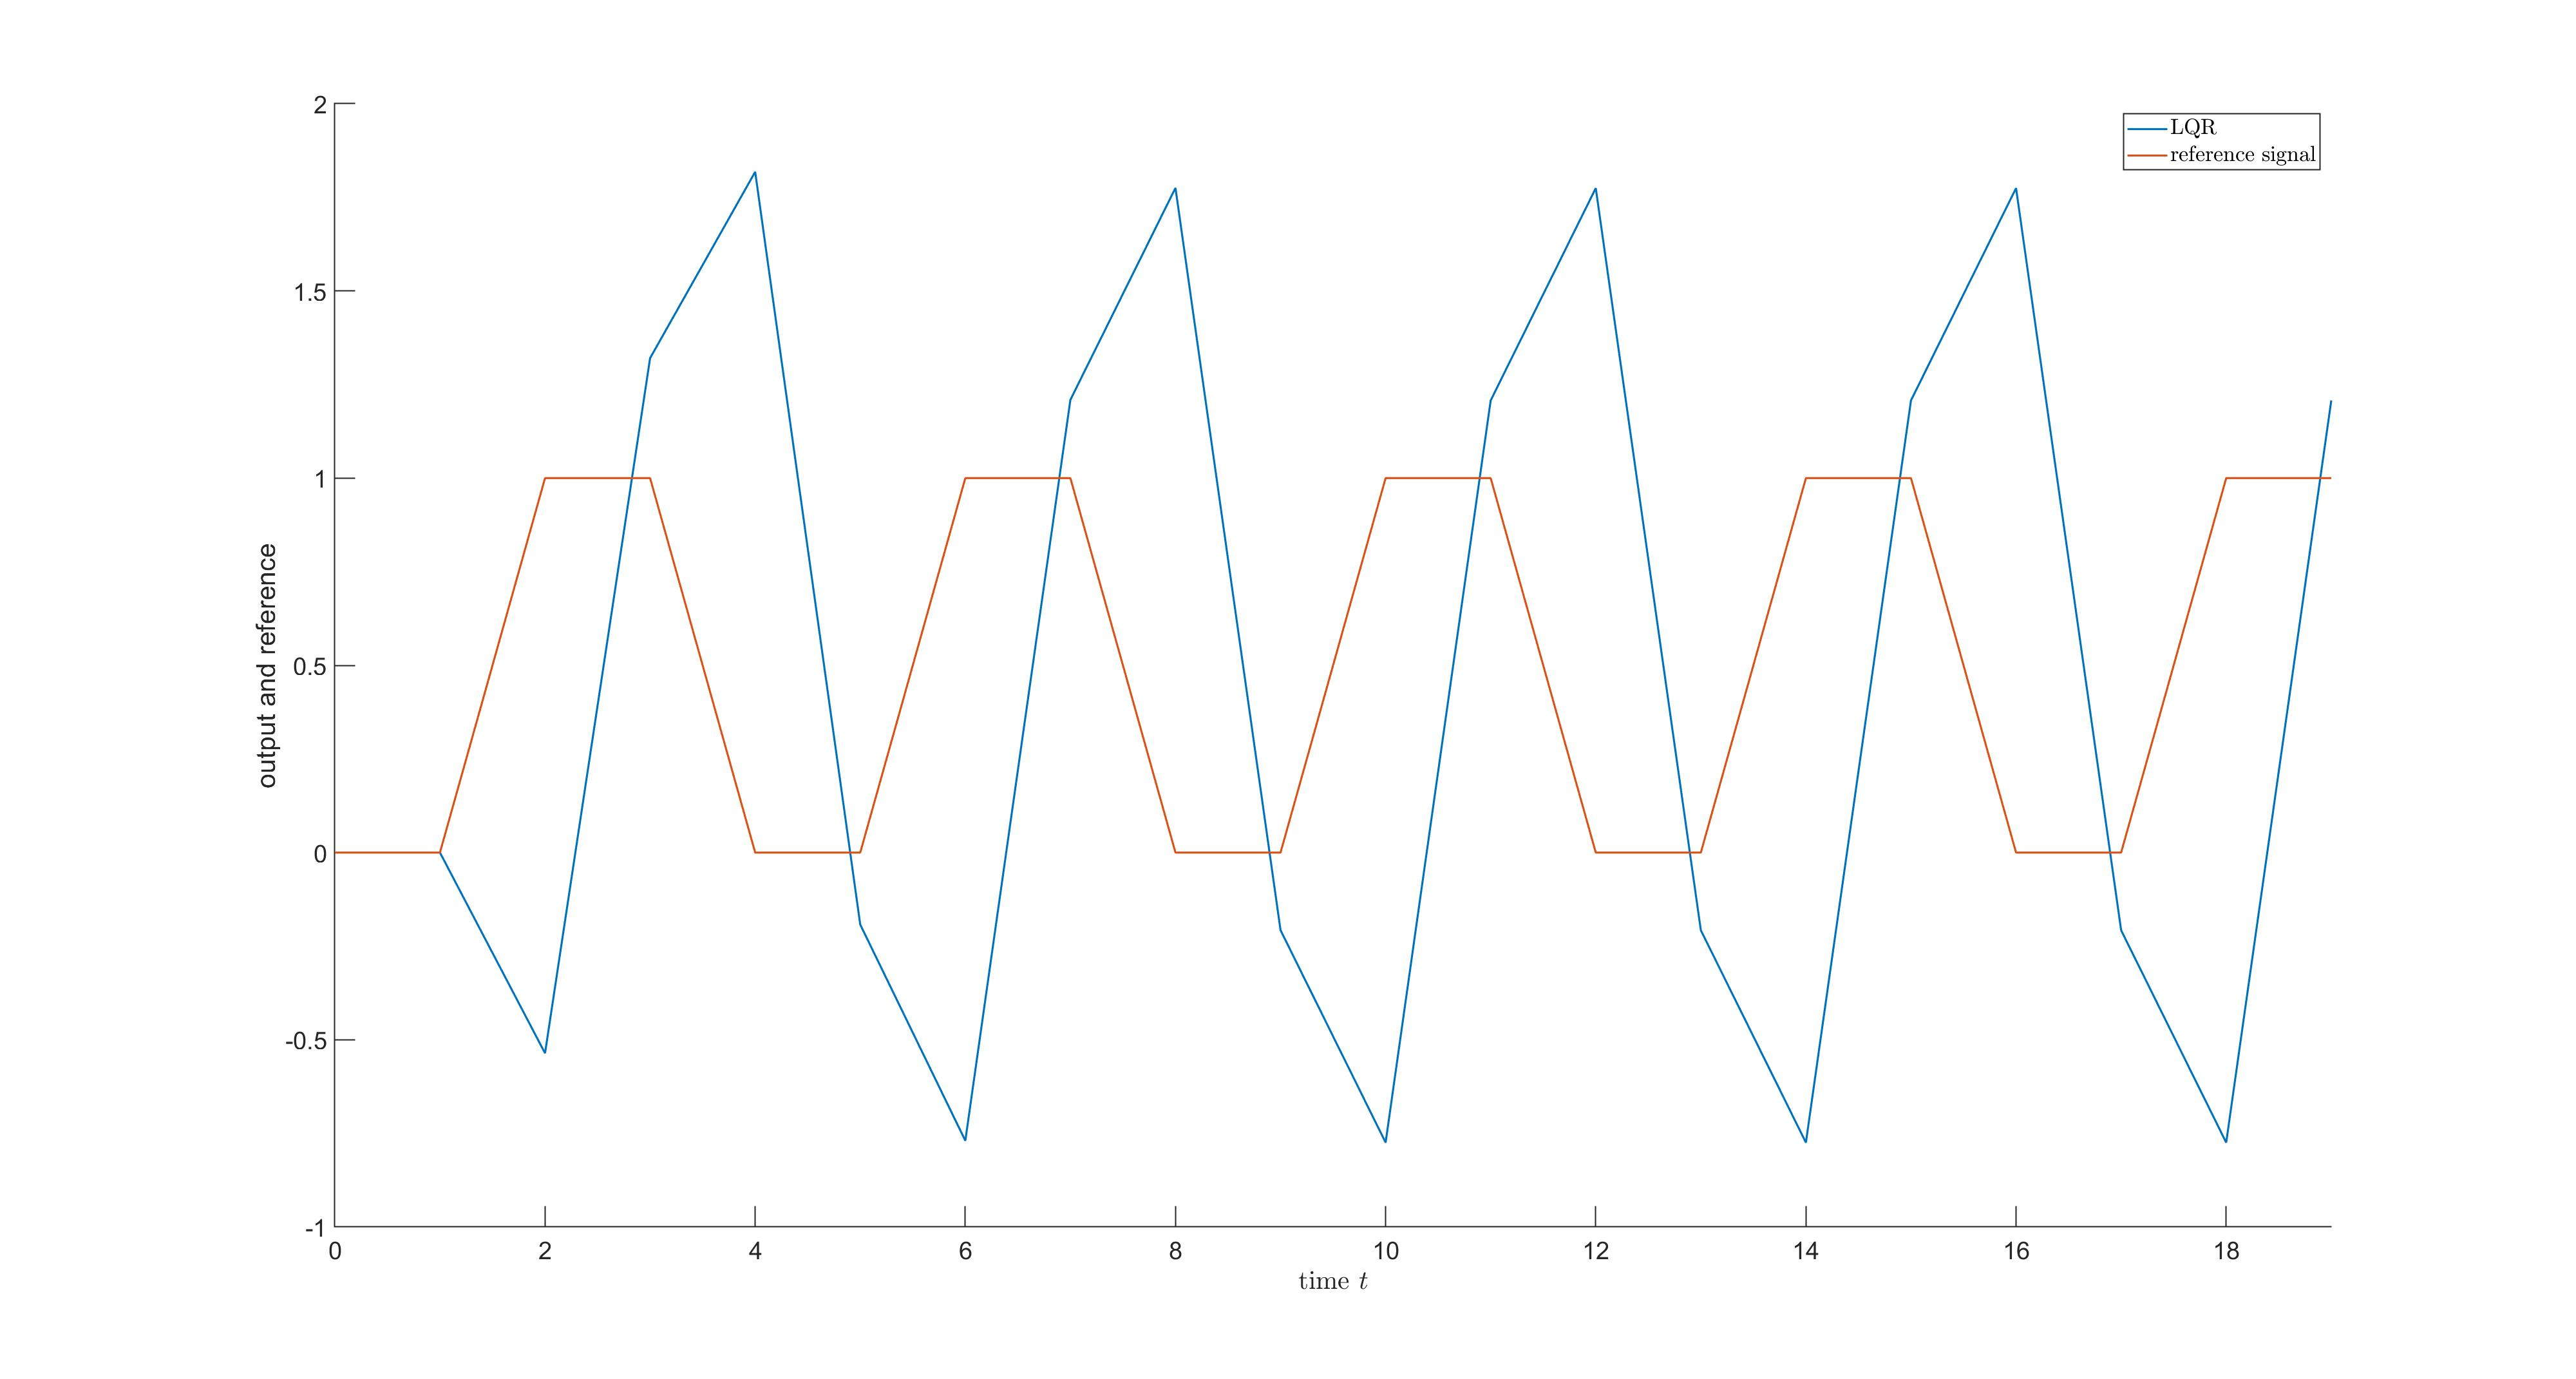
\includegraphics[width=\textwidth]{fig/Ex1_LQR.jpg}
	\caption{Tracking with LQR controller for system \eqref{eq:ILC:Sys_ex1}}
	\label{img:ILC:LQR_control}
\end{figure}
\end{exam}



As one can see, the tracking in Example \ref{ex:ILC:LQR} is not perfect. However, we can extract a bunch of information from this controlled system. For example, we get the input and output sequences 
\begin{align}
&\{u(0), \, u(1), \,  u(2) \, \dots , \, u(N)\} \subset \R^l \label{eq:ILC:u_seq}, \\
&\{y(0), \, y(1), \, y(2) , \, \dots , \, y(N)\}\subset \R^m.\label{eq:ILC:y_seq}
\end{align}
On the finite time horizon of interest the behavior of system is described by the finite input and output sequences. It seems to be an advantage. 

If we put the signals we got from simulation together, we get a large, but finite dimensional vector. That means, the standard tools from linear algebra can be applied. 

As a matter of fact, we can express our whole simulated system as a linear equation. We call such vectors \textit{supervectors}, and the whole system is said to be \textit{lifted}. This notation can describe the whole system dynamic in a compact form, and is a useful tool for ILC algorithms. 

\section{Supervector description} 

\begin{defi}
	Let $\{s(0), s(1), s(2), \dots s(N)\} \subset \R^{d}$ be a finite sequence. Then the supervector corresponding to this sequence is denoted by $s$ and is defined as 
\begin{align}
s: = \begin{pmatrix}
s(0) \\ s(1) \\ s(2) \\ \vdots \\ s(N)
\end{pmatrix}.
\end{align}
\end{defi}

In this way we define the supervectors $u \in \R^{l(N+1)} $ and $e$, $y$, $r \in \R^{m(N+1)}$. 
Analogously, we determine supervectors $r\in \R^{m(N+1)}$ and $e\in \R^{m(N+1)}$. 

For system \eqref{eq:GP} the relation between $u$ and $y$, and the error $e$ can be written in a linear matrix form 
\begin{align}
\label{eq:Gu + d}
y &= Gu + d, \\
e &= r - y.
\end{align}
The \textit{supermatrix} $G$ represents the state-space model and is given via  
\begin{align}
\label{eq:Gmatrix}
\begin{split}
G &= G(A,B,C,D) = \\
&=  \begin{pmatrix}
D & 0 & \cdots & 0 & 0 & 0 \\
CB & D & \cdots & 0 & 0 & 0\\
CAB & CB & \cdots & 0 & 0 & 0\\
\vdots & \vdots & \ddots & \vdots  & \vdots & \vdots \\
CA^{N-2} B & CA^{N-3} B &\dots &CB & D& 0\\
CA^{N-1} B & CA^{N-2} B &\dots &CAB & CB& D\\
\end{pmatrix} \in \R^{m(N+1)\times l(N+1)}.
\end{split}
\end{align}
The vector $d$ depends on the initial condition $x_0$:
\begin{align}
d = d(C,A,x_0) = \begin{pmatrix}
C x_0 \\ CA x_0 \\ CA^2 x_0 \\ \vdots \\ CA^Nx_0
\end{pmatrix} \in \R^{m(N+1)}.
\end{align}

The stability requirement for $A$ is highlighted here. In opposite to vast values for unstable matrices, we get very small terms if $N \gg 1$. Intuitive, this terms can be neglected for all $p > p^\star$ for some $1<p^\star<N$. This is usable since we can apply the sparse matrices. In the Chapter \ref{ch:Allpication} we will see, that a good estimation can be derived. 

For the system \eqref{eq:Gu + d}, the tracking problem seems to be straightforward.
If we know the reference signal $r$, we can find a perfect solution by choosing 
\begin{align}
u_\infty = G^{-1} r -d.
\end{align}

However, this choice does not look greatly credible. 
For example, if our measurements are disturbed by noise, we get the output signal
\begin{align}
y + \varepsilon w = G u_\infty + d + \varepsilon w = r + \varepsilon w \neq r,
\end{align}
for some non-zero vector $w \in \R^{m(N+1)}$ and small $\varepsilon > 0$. 

Also for uncertain models this method might be not applicable. 
If we could reformulate this idea in a more robust way, we may get a good and simple applicable algorithm, which we call the \textit{Inverse Model Algorithm.}

\section{Inverse Model Algorithms}

\begin{alg}
	\label{alg:ILC:IA}
	Let the matrix $D$ in \eqref{eq:GP} have an inverse. Then the matrix $G = G(A, B, C, D)$ is non-singular as well, and the Inverse Model Algorithm (IA) is given via input update law 
	\begin{align}
	\label{eq:errRightInv}
	\begin{split}
	u_{k+1} &= u_k + \beta G^{-1} e_k, \\
	u_0 & \in \R^{l (N+1)},
	\end{split}	
	\end{align}
	with error evolution
	\begin{align}
	\label{eq:Alg:e_k+1 = (1 - beta) e_k}
	\begin{split}
	e_{k+1} &= (1- \beta) e_{k}, \; k\geq 0, \\
	e_0 &= r -  Gu_0 -d.
	\end{split}
	\end{align}
	In particular, $(e_k)_{k\geq 0}$ converges to zero for $k \to \infty$ for any initial error $e_0 \in \R^{m(N+1)}$ if and only if 
	\begin{align*}
	0 < \beta < 2.
	\end{align*}
\end{alg}
\begin{proof}
	Firstly, the matrix $G$ has lower triangular structure, with the matrix $D$ on its diagonal. Hence, $\det(G) = \det(D)^{N+1}$, which is non-zero if and only if $D$ has full rank. 
	Taking the limit over relation \eqref{eq:Alg:e_k+1 = (1 - beta) e_k} results in
	\begin{align}
	\lim_{k \to \infty} e_{k+1} = \lim_{k \to \infty}(1- \beta) e_{k} = \lim_{k \to \infty}(1 - \beta)^k e_0.
	\end{align}
	Choosing $0<\beta < 2$ yields the proof. 
\end{proof}

For $\beta$ close to 0 or 2, we get slower convergence and better robustness. For $\beta = 1$ we get convergence in one iteration, but this choice might be non-robust \cite{ILC}, pp 149, 152-155.

We apply this algorithm on the system from Example \ref{ex:ILC:LQR} to see the algorithm performance. 

\begin{exam}
	\label{ex:ILC:badIA}
	In the system \eqref{eq:ILC:Sys_ex1} the matrix $D = 2$ is invertible, and we can apply IA. We choose as $u_0$ the input sequence of LQR controller, and $\beta = 0.1$. Convergence to 0 with tolerance $10^{-8}$ is achieved after 74 iterations.The result is illustrated in Figure \ref{img:ILC:Ex1_IA}
			
	\begin{figure}[ht]
		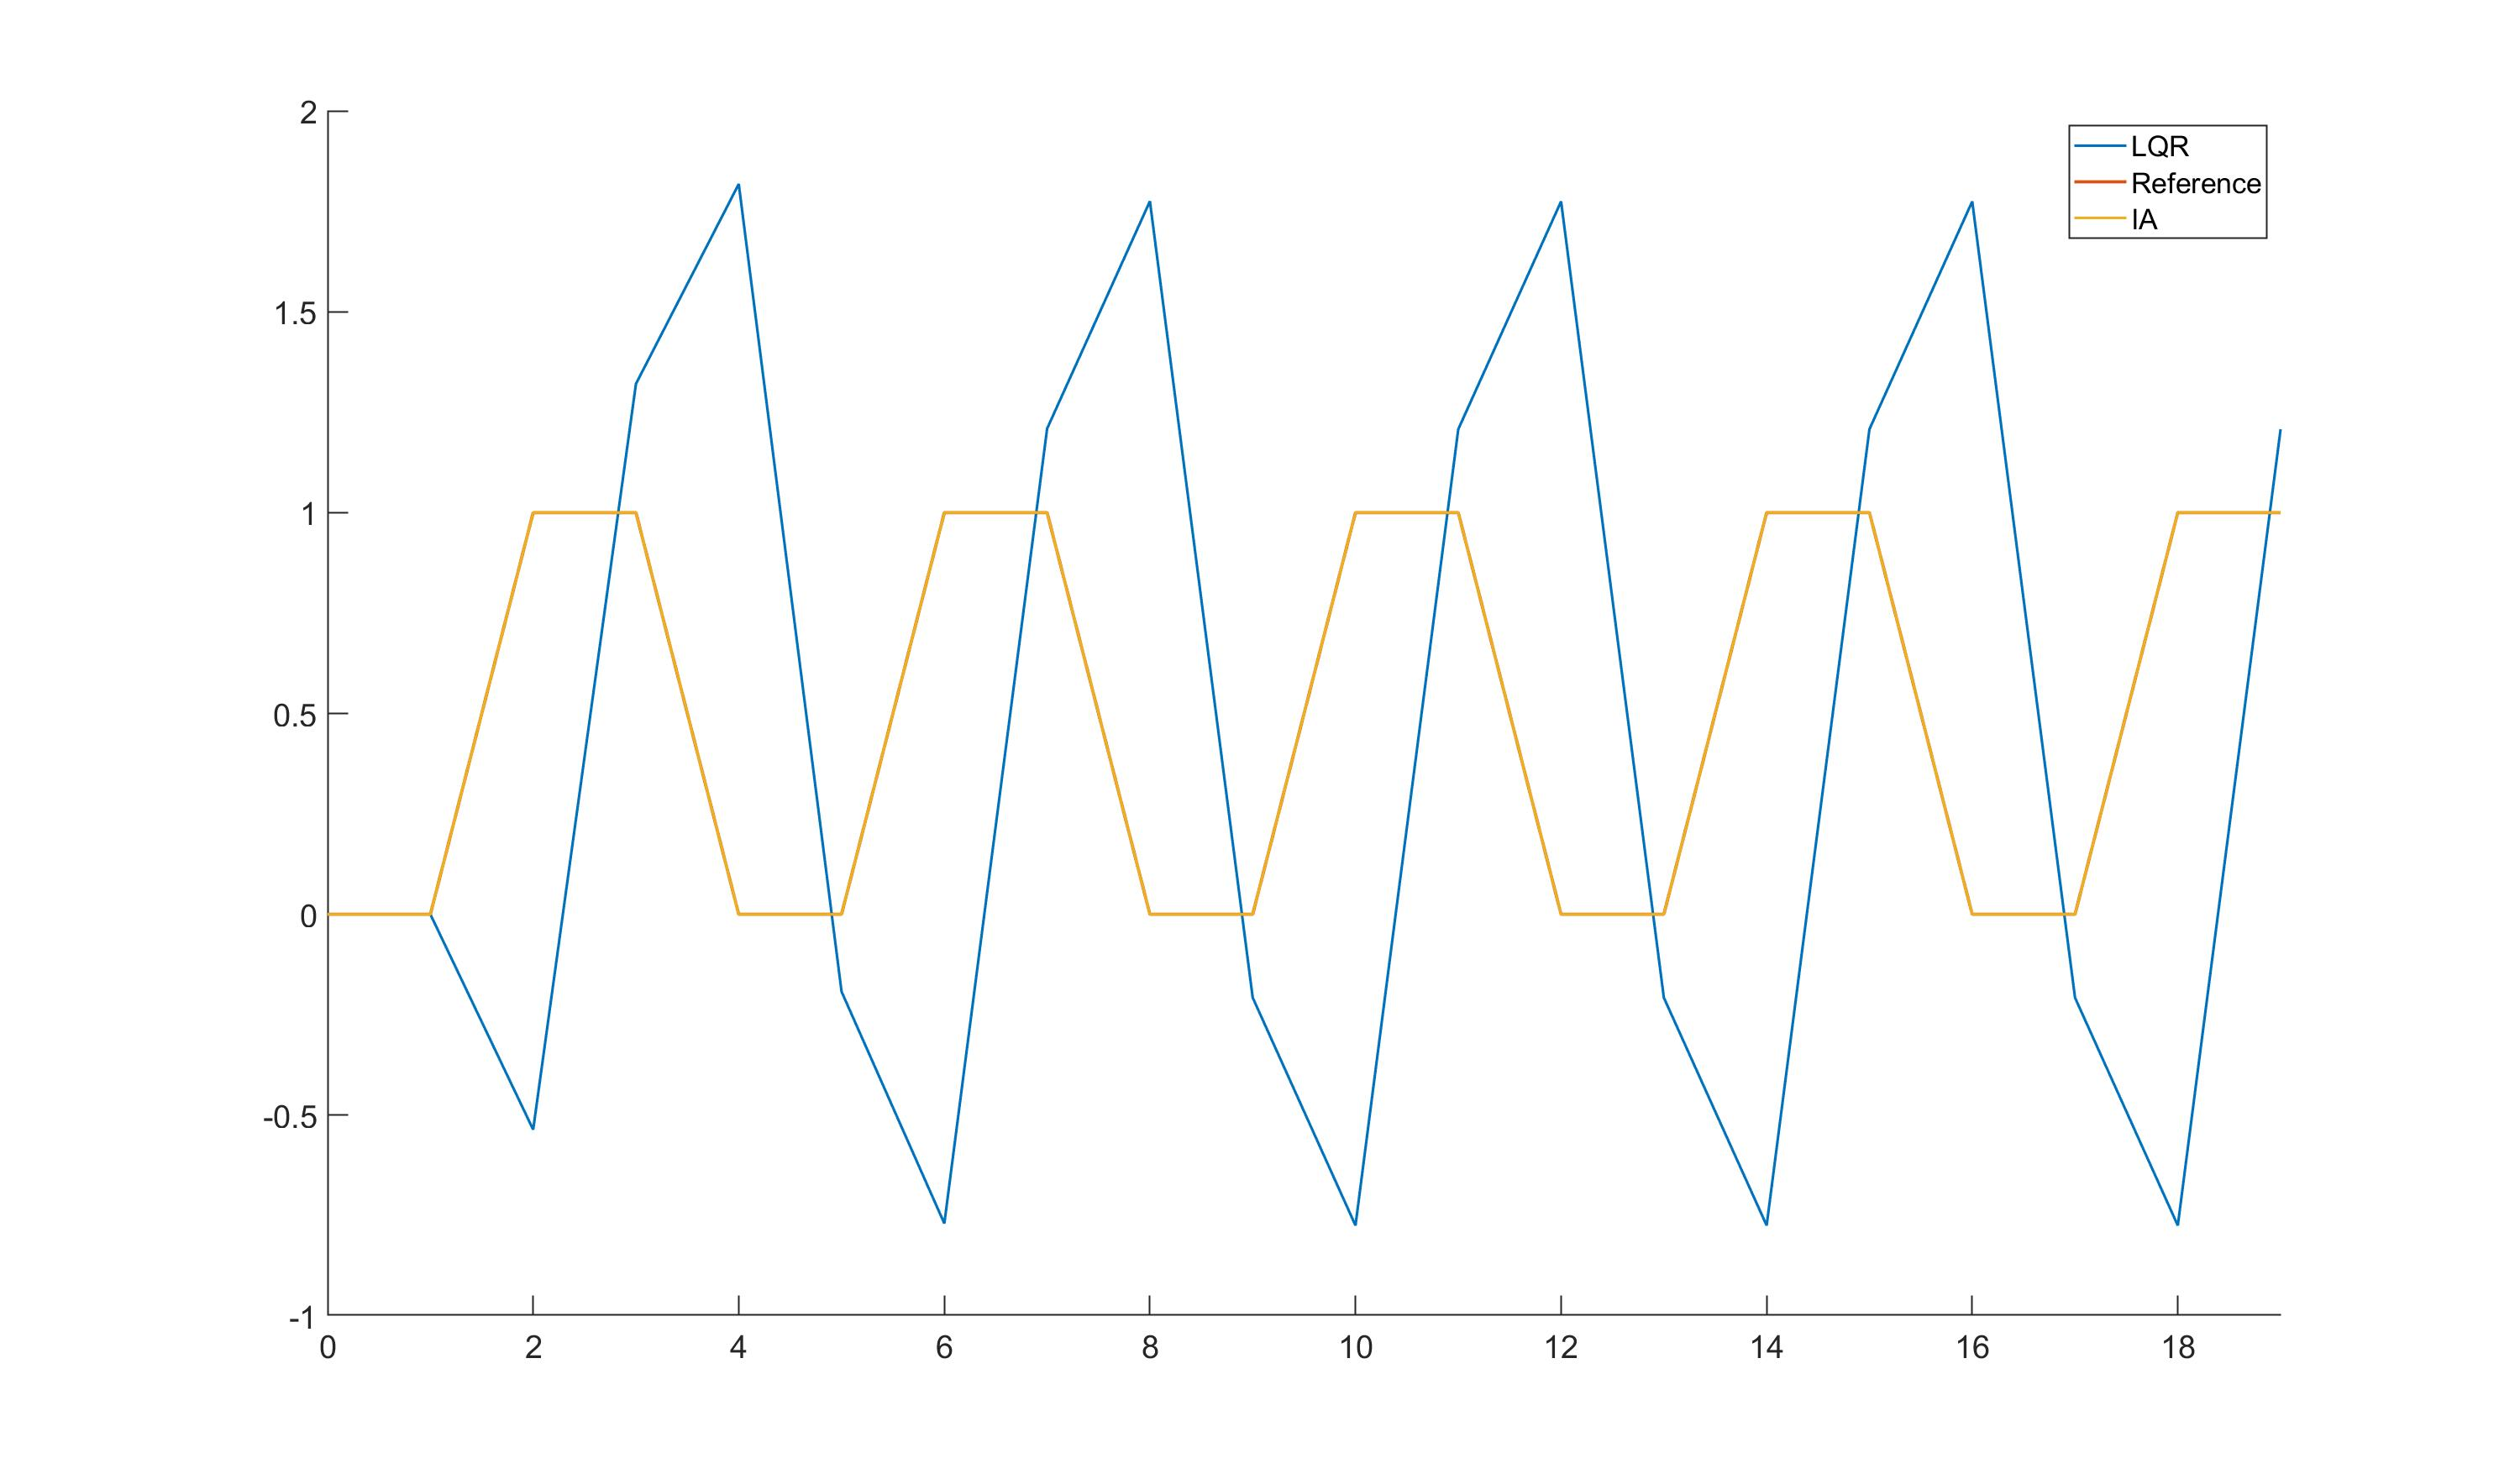
\includegraphics[width=\textwidth]{fig/Ex1_IA.jpg}
		\caption{Tracking with LQR Controller (without ILC Algorithm), and tracking with IA for the system \eqref{eq:ILC:Sys_ex1} for $N = \IAgood$}. 		\label{img:ILC:Ex1_IA}
	\end{figure}
	
	But if we try to increase the length of the time horizon $N$, for example to \IAbad steps, we can see a wrong system behavior (Figure \ref{img:ILC:Ex1_IAbad}). 
		
			\begin{figure}[ht!]
			\centering
			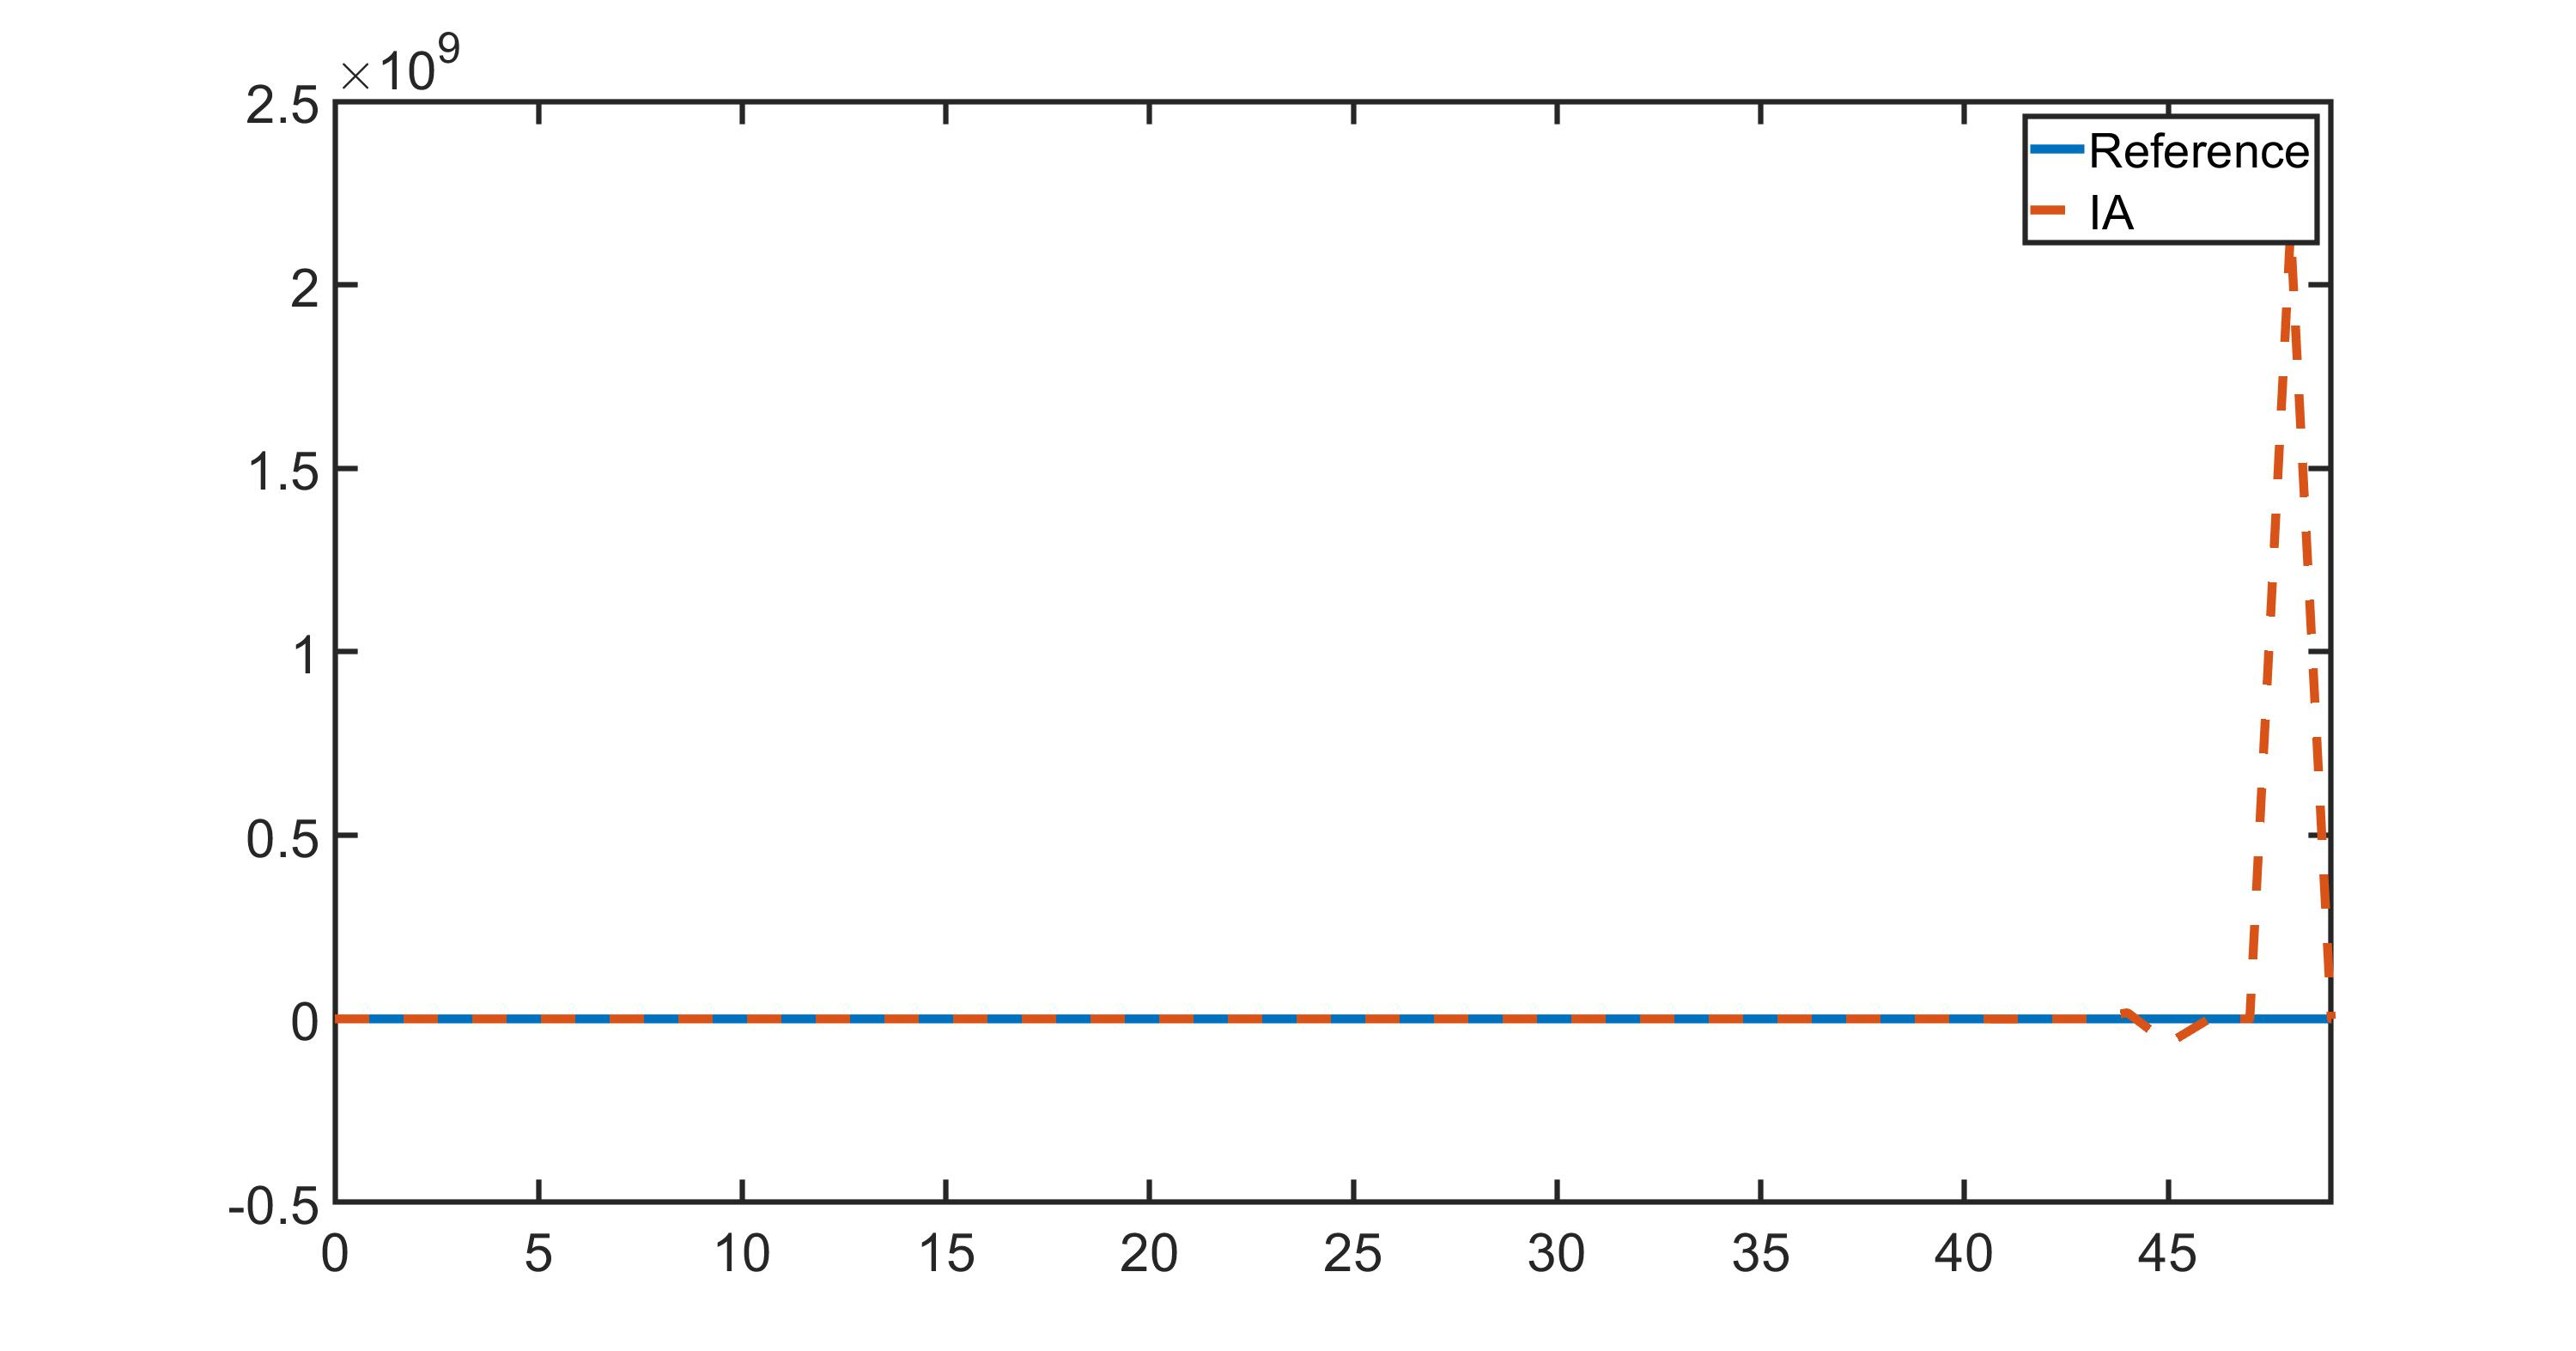
\includegraphics[width=\textwidth]{fig/Ex1_IAbad.jpg}
			\caption{Tracking with IA for the system \eqref{eq:ILC:Sys_ex1} for $N = \IAbad$}
			\label{img:ILC:Ex1_IAbad}
		\end{figure}
	
	The reason is the condition number of the matrix $G$, which equals \badCondNb. We see: even for a triangular matrix with non-zero eigenvalues, the matrix inversion can be numerically unstable.
		
		
\end{exam}

The Inverse Model Algorithm sets up very strong requirements: the matrix $G$ should be non-singular, and its condition number must be small enough we can compute a numerically stable inverse. 
We can modify this algorithm by taking the Moore-Penrose inverse. This is the so-called pseudo inverse, which is uniquely defined and can be computed for all matrices \cite{LAAG}. 

\begin{defi}
	For a matrix $G \in \R^{m(N+1) \times l(N+1)}$ a psedo inverse is defined by matrix $G^+ \in \R^{l(N+1) \times m(N+1)}$, satisfying the criteria: 
	\begin{enumerate}
		\item $G G^+ G  = G $
		\item $G^+ G G^+ = G^+$
		\item $(G G^+)^T = G G^+$
		\item $(G^+ G)^T = G^+ G$
	\end{enumerate}
\end{defi}



\begin{alg}
	\label{alg:ILC:PIA}

	The Pseudo Inverse Model Algorithm (PIA) is given via input update law 
	\begin{align}
	\label{eq:ILD:errPIA}
	\begin{split}
	u_{k+1} &= u_k + \beta G^{+} e_k, \\
	u_0 & \in \R^{l (N+1)},
	\end{split}	
	\end{align}
	with error evolution
	\begin{align}
	\begin{split}
	e_{k+1} &= (1- \beta G G^+) e_{k}, \; k\geq 0, \\
	e_0 &= r -  Gu_0 -d.
	\end{split}
	\end{align}

	Monotonic convergence to 
	\begin{align}
	\label{eq:ILC:einfPIA} 
	e_\infty  = \lim_{k\to\infty} e_k = P_{\ker[G^+]}e_0,
	\end{align} 
	is guaranteed if
	\begin{align*}
	0 <\beta < 2
	\end{align*}
	$P_{\ker[G^+]}$ denotes the positive orthogonal projection operator onto $\ker[G^+]$.
	In particular, the zero convergence is attainable, if and only if the tracking signal $r$ is feasible, that is there exists an input $\hat u$, such that $r = G \hat u$. %$e_0 \in \im [G G^\star]$. 
\end{alg}
\begin{proof}
	
	Recap the relation $(GG^+)^2 = GG^+GG^+ = GG^+$ the error evolution formula \eqref{eq:ILC:errevol_PIA} can be proven by mathematical induction: 
	
	for $k = 1$ it follows: 
	\begin{align*}
	e_1 = (I - \beta G G^+)e_0 = (I + GG^+ - GG^+ - \beta G G^+)e_0 = (I + \left[(1 - \beta) + 1\right]GG^+)e_0.
	\end{align*}
	
	For $k \in \N$  
	\begin{align*}
	e_{k+1} &= ( I - \beta G G^+)e_k = ( I - \beta G G^+) (I+  \left[(1-\beta)^{k-1} - 1\right] G G^+) e_0 = \\
	& = \left(I - \beta G G^+ + (1-\beta)^{k-1}GG^+ - GG^+ - \beta GG^+\left[(1 - \beta)^{k-1} - 1\right]GG^+\right)e_0=\\
	& = \left(I - (\beta - (1-\beta)^{k-1} + \beta\left[(1 - \beta)^{k-1} - 1\right])G G^+\right)e_0\\
	& = \left(I - \left(\beta - (1-\beta)^{k-1} + 1 + \beta(1-\beta)^{k-1} - \beta\right)GG^+\right)e_0\\
	& = (I+  \left[(1-\beta)^k - 1\right] G G^+) e_0
	\end{align*}
	
	To prove \eqref{eq:ILC:einfPIA}  recall that 
	\begin{align*}
	\R^{m(N+1)} = \im(G)\oplus \ker (G^+),
	\end{align*}
	$\oplus$ denotes here the direct sum of two vector spaces. 
	Hence $e_0$ can be written as 
	\begin{align*}
	e_0 = G w_0 + v_0,
	\end{align*}
	where $v_0 = (I - G G^+)e_0 \in \ker (G^+)$  is uniquely defined and $w_0 = G^+ e_0 \in \R^{l(N+1)}$. It follows: 
	\begin{align*}
	e_{k} = (1+ \left[(1 - \beta)^{k-1} - 1\right]GG^+)e_0 = (1-\beta)^{k-1} G w_0 + v_0.
	\end{align*}
	Then for $\beta \in (0,2)$ the error $e_k$ converges to $v_0$ for $k \to \infty$. 
\end{proof}

\begin{exam}
	\label{ex:ILC:PIA}
	We calculate a solution for \eqref{eq:ILC:Sys_ex1} with PIA, and illustrate it in Figure \ref{fig:ILC:Ex1_PIA}. 	
	This time the tracking signal and system output fit well despite the large condition number. However, a deviation can be observed at the beginning, which causes the bad invertability of the matrix $G$. 
	  
	\begin{figure}[ht!]
		\centering
		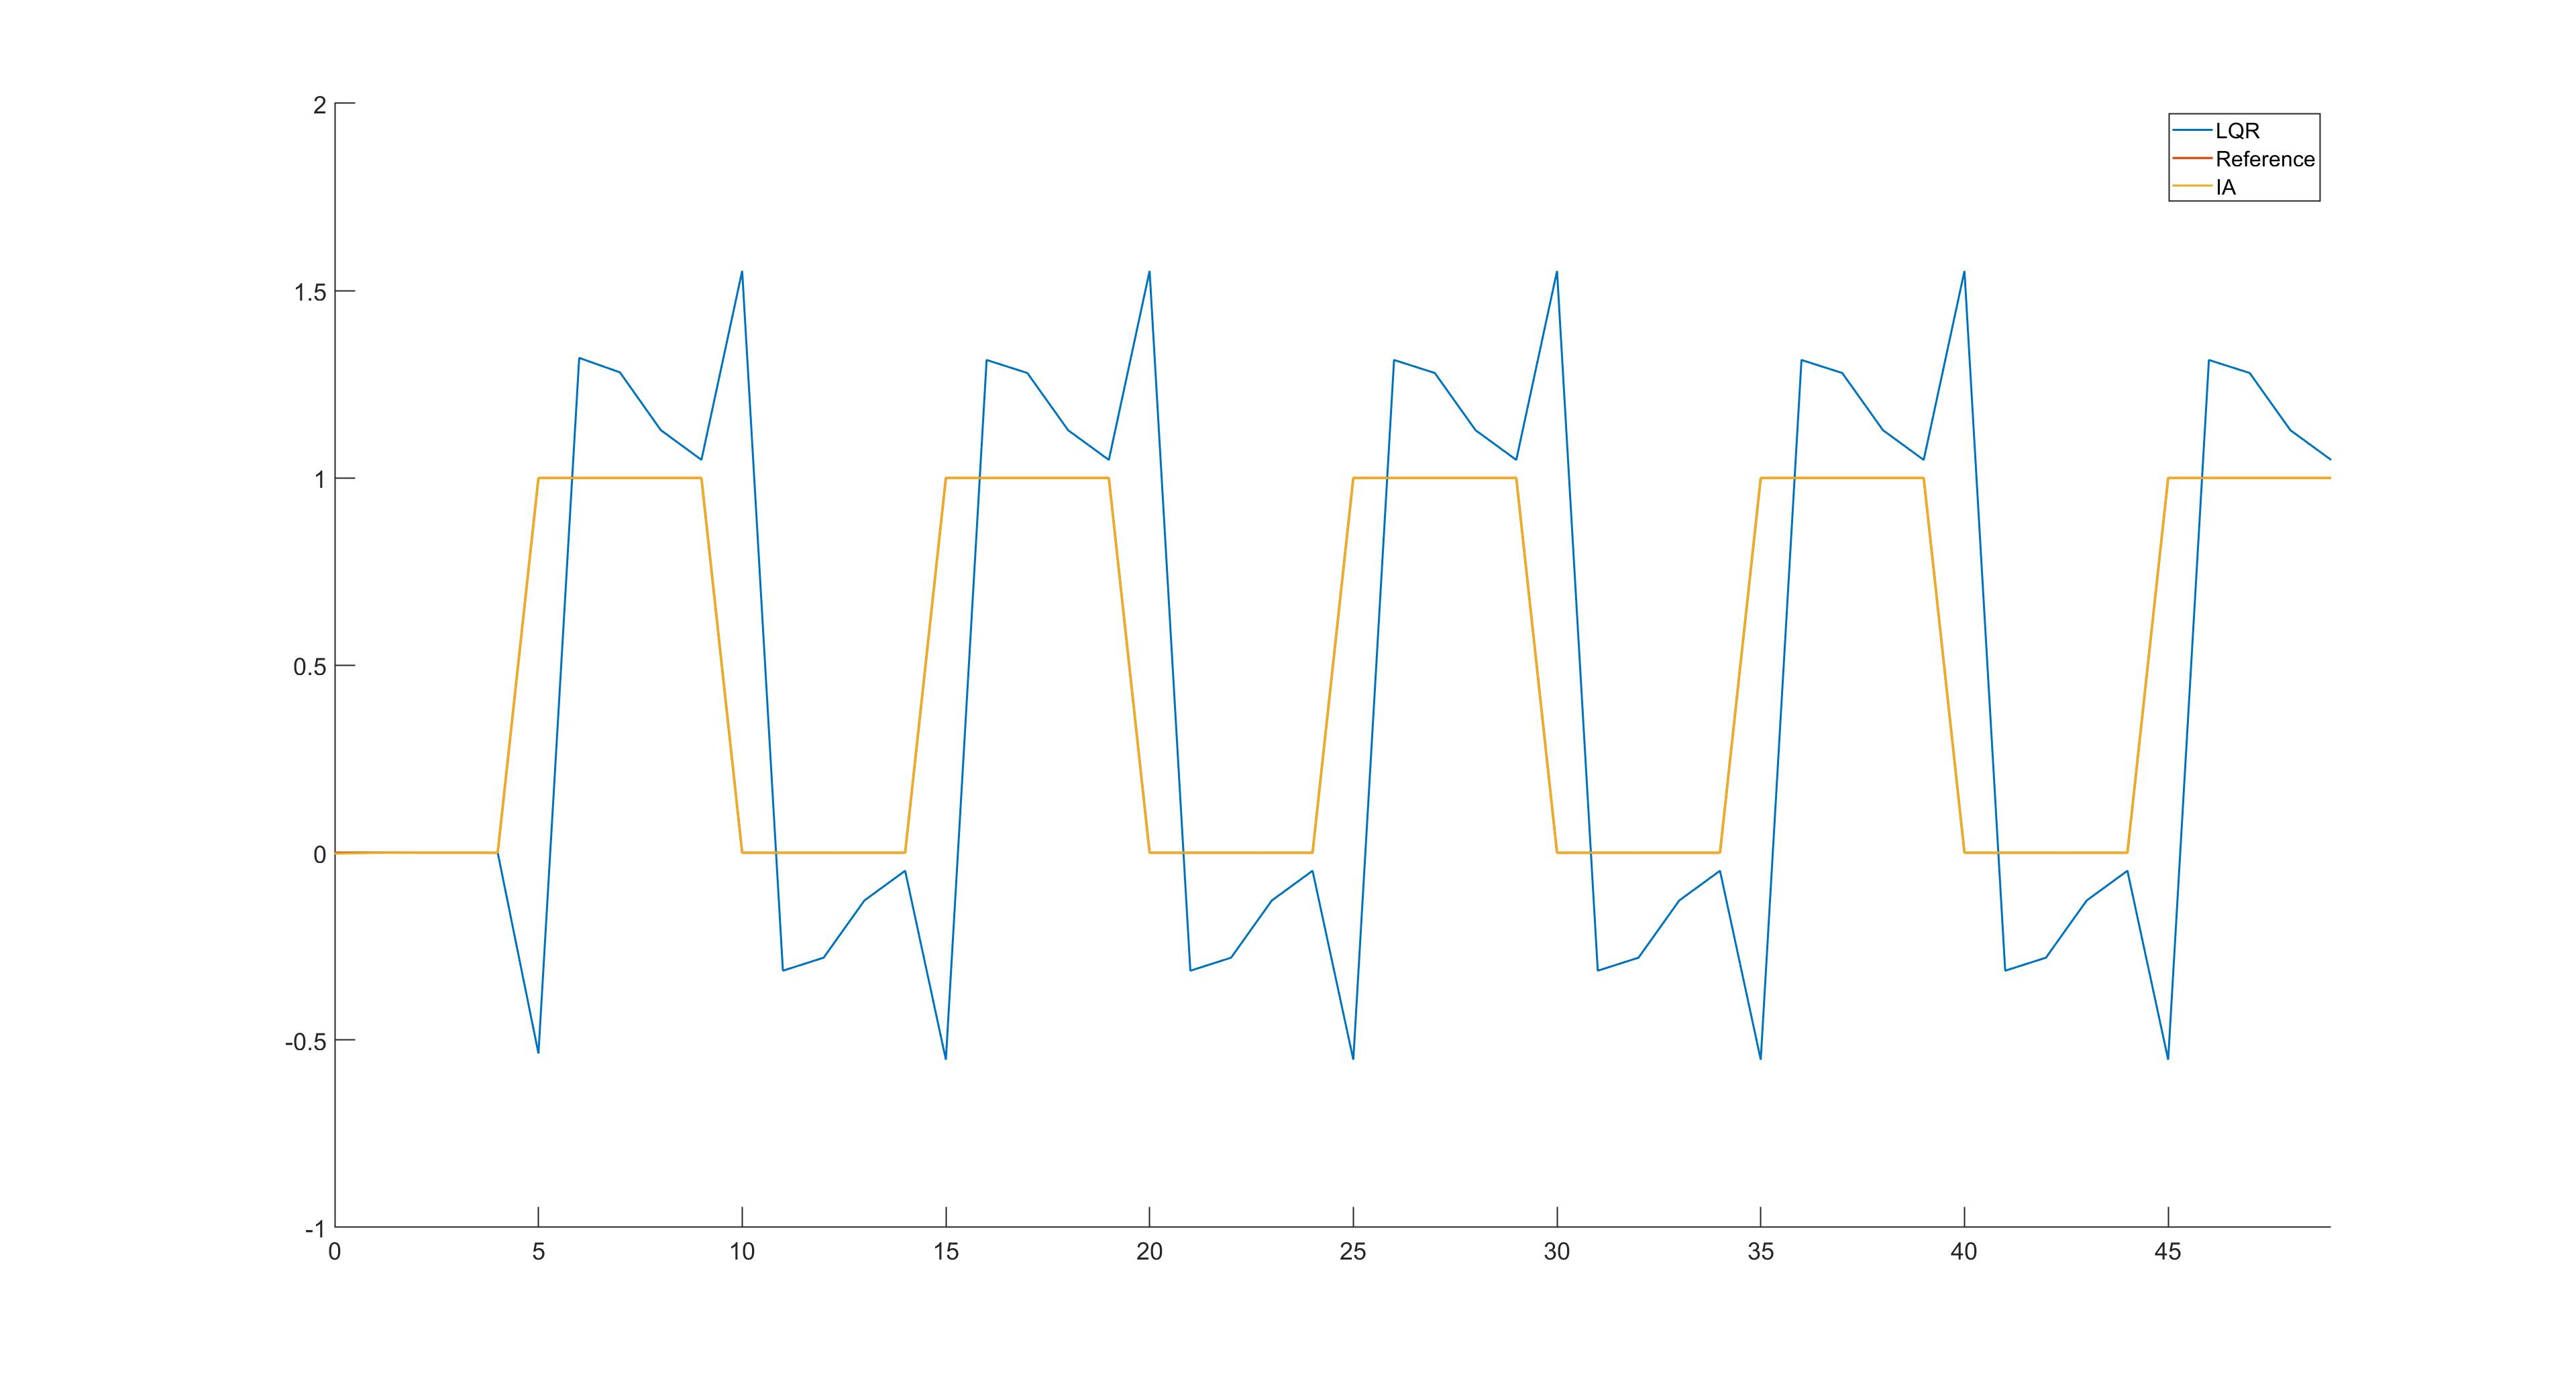
\includegraphics[width=\textwidth]{fig/Ex1_PIA.jpg}
		\caption{Reference signal tracking with LQR and PIA for the sysytem \eqref{eq:ILC:Sys_ex1} for $N = \IAbad$ }
		\label{fig:ILC:Ex1_PIA}
	\end{figure}
\end{exam}


We can replace the use of pseudo inverse by taking a left or right inverse, if it exists. 
However, it  only makes sense if the calculating afford or numerical stability are better for left or right inverse calculation. 

The pseudo inverse has its advantage to equal the right/left inverse, if it exists. Moreover, for right/left inverse we need to restrict the rank requirements, as it exists not for every matrix. 
The algorithm in this formulation can be applied for any matrix $G$. 

The Algorithm \ref{alg:ILC:IA} is a special case of PIA. However, numerically the use of inverse matrix might be more desirable since the calculation effort, if the condition number is not large. 

(Pseudo) Inverse Algorithm belongs to the class of so-called Unit Memory Algorithms -- these are the algorithms we assume to  ''remember'' the last trial. 

\section{Unit Memory Algorithm}

We are interested in  the processes, which are executed repetitively. Let $k = 0, \, 1, \, 2, \, \dots $ be the number of completed iterations. Then we get a system 
\begin{align}
\label{eq:unitMemory}
\begin{split}
y_{k} &= G u_k + d,  \\ %& &\text{ (The Input Update Rule)} 
e_k &= r - y_k, 
\end{split}
\end{align}
$u_{0} \in \R^{l(N+1)},  \; k =0, \,  1, \, 2, \dots $.
%This is again a discrete-time system, with time increment $k$. 

To achieve a good tracking at trial $k$ we need to ensure that the norm $||e_k||$ is small. 
The tracking behavior improves for consecutive iterations if the sequence $||e_k||$ is monotonically decreasing, i.e., 
\begin{align}
||e_{k+1} || < ||e_k|| \text{ for all } k \geq 0.
\end{align}
Note that in this case the sequence $||e_k||$ is guaranteed to converge. If the sequence even converges to zero we say that perfect tracking is achieved asymptotically.


We have already seen, that it is not always possible to achieve zero convergence. In Algorithm \ref{alg:ILC:PIA} the perfect tracking is possible, if the reference signal $r$ is feasible -- that is, there exists an input signal $u_\infty$, such that $r = G u_\infty + d$. In common the convergence properties can also depend on the choice $u_0$.

%the monotonic convergence to some $e_\infty \in \R^{m(N+1)}$ is desirable :
%\begin{align}
%\lim_{k \to \infty} e_k = e_\infty, \text{ and } ||e_{k+1} || \leq ||e_k|| \text{ for all } k \geq 0.
%\end{align}

%First we try to formulate an iteration law for the input signal, and calculate then the error sequence as 
%\begin{align}
%e_k = r - y_k = r - G u_k - d, k \geq 0.
%\end{align}

We assume linear dependency of $u_{k+1}$ upon $u_k$ and $e_k$ for $k \geq 0$, and define the following algorithm using feedback control. 
\begin{alg}
	\label{alg: unitMemory}
	The Unit Memory Algorithm is given via input update law 
	\begin{align}
	\label{eq:clPlant}
	\begin{split}
	u_{k+1} &= u_k + K e_k, \\
	& u_0 \in \R^{l (N+1)}.
	\end{split}
	\end{align}	 
	The error dynamic is then given via
	\begin{align}
	e _{k+1} &= (I - G K) e_{k}, \; k \geq 0,\\
	e_0 &= r -  Gu_0 -d.
	\end{align}
%	since 
%	\begin{align}
%	\begin{split}
%	e_{k+1} &=  r - y_{k+1} = r - G u_{k+1} - d =\\
%	&= r - Gu_k - G Ke_k - d = e_k - G Ke_k, \; k\geq0.
%	\end{split}
%	\end{align}
	$K \in \R^{l(N+1) \times m(N+1)}$ is called \textbf{learning matrix}. 
\end{alg}

To ensure the stability of the algorithm, it is enough to consider the iteration process 
\begin{align}
\label{eq:e_k}
e_{k+1} = (I - G K) e_k = (I - G K)^k e_0  : =  L^k e_{0}, \; k \geq 0.
\end{align}

That it is a discrete time dynamical system over $k$. We can reformulate our goal as follows: find some matrix $K \in \R^{l(N+1) \times m (N+1)}$, which renders \eqref{eq:e_k} stable. %In other words, we are looking for a stabilizing controller $K$. 

If we rewrite our system as
\begin{align}
\label{eq:ILC:e_kPlant}
\begin{pmatrix}
e_{k+1} \\ e_k
\end{pmatrix} = 
\left(
\begin{array}{c|c}
I & -G \\\hline I & 0
\end{array}\right) \begin{pmatrix}
e_k \\ v_k 
\end{pmatrix},
\end{align}
our problem reduces to finding a stabilizing controller $K$  with 
\begin{align}
v_k = K e_k.
\end{align} 

We know how to work with such systems -- for example, LQR controller provides a good solution. This is a reliable method, but since the matrix $G$ can have large dimension, it also can be costly. Often we can achieve good results with much more simple methods. For example, we can reduce the number of parameters to be chosen. 

In the Algorithms \ref{alg:ILC:IA} and \ref{alg:ILC:PIA} we chose a fixed matrix $K_0$ as the (pseudo) inverse of $G$, and left the parameter $\beta$ to decide on. So, we reduced the number of degrees of freedom to 1, and still get satisfying results.


However, as we have seen in Example \ref{ex:ILC:badIA}, the calculation of the  inverse matrix is not the most reliable method. The pseudo inverse refers better results, but is also much more expensive. 

An algorithm, which does not require the model inversion, might be here of use. 

	 \section{Gradient Algorithms}
We want a new algorithm to render monotonic convergence. 
The direct calculation provides 
\begin{align}
\label{eq:monConv}
||e_{k+1}|| < ||e_k|| \text{ for all } k >0,
\end{align}

in some norm $|| \cdot || $ in $\R^{m(N+1)}$. 

We chose positive definite weighting matrices $Q(t)$ and $R(t)$, $t = 0, 1, 2, \dots ,N$, and define the scalar products
\begin{align}
\label{eq:SkPrQR}
\langle y,z\rangle_Q = \sum_{t = 0}^N y(t)^TQ(t)z(t), \; \langle u,v\rangle_R = \sum_{t = 0}^N u(t)^T R(t) v(t),
\end{align}
with $y(t), z(t) \in \R^{m}$, $u(t), v(t) \in \R^l$ for $t = 0,1,2, \dots, N$.

We denote with $||\cdot||_Q$ and $||\cdot||_R$ the associated norms, and set
\begin{align*}
G^\star &= R^{-1} G^T Q \text{ for all } G \in \R^{m(N+1)\times l(N+1)},\\
K^\star &= Q^{-1} K^T R \text{ for all } K \in \R^{l(N+1)\times m(N+1)},
\end{align*}
where 
\begin{align}
Q := \diag(Q(0), Q(1), Q(2) ,\dots, Q(N)) \text{ and } R:= \diag(R(0), R(1), R(2), \dots, R(N)).
\end{align}
%In the same way, we can define 
%\begin{align}
%L^\star &= Q^{-1} L^T Q \text{ for all } L \in \R^{m(N+1)\times m(N+1)} \text{ and }\\
%M^\star &= R^{-1} M^T R \text{ for all } M \in \R^{l(N+1)\times l(N+1)}.
%\end{align}

Recall, that for $R = I$ and $Q = I$ the matrices $G^\star$ and $K^\star$ are just the conjugate transpose. The notation from above can be seen as conjugate transpose in the vector space with scalar products \eqref{eq:SkPrQR}.

Applying the weighted norms on \eqref{eq:monConv} provides
\begin{align}
\begin{split}
||e_{k+1} ||_Q^2 &= ||e_k - G K e_k||_Q^2 = ||e_k||_Q - 2\langle e_k , G K e_k \rangle_Q + ||G K e_k||_Q^2 \\ 
&< ||e_k||_Q^2, \text{ if } ||GK e_k||_Q^2 < 2 \langle e_k, GK e_k\rangle_Q. 
\end{split}
\end{align}

The last inequality is equivalent to 
\begin{align}
e_k^T K^T G^T Q GK e_k < 2 e_k^T Q GK e_k.
\end{align}

If we set $K = \beta G^{\star}$ this is implicated by 
\begin{align}
\label{eq:ILC:SDA_Herleitung}
\beta^2 (G G^{\star})^T Q (G G^{\star}) \prec \beta Q G G^{\star} + \beta (Q G G^{\star})^T.
\end{align}

Since the matrix $Q$ is positive definite, we can find a positive definite 	 matrix $Q^{1/2}$, such that $Q = Q^{1/2}Q^{1/2}$. 

We write $Q^{-1/2}$ for $\left(Q^{1/2}\right)^{-1}$, and define a matrix 
\begin{align}
H :=  Q^{1/2} G G^\star Q^{-1/2}. 
\end{align}
The matrix $H$ has the same eigenvalues as $G G^{\star}$, as for its characteristic polynomial holds 
\begin{align}
\begin{split}
\det (I - \lambda H) &= \det \left(I - \lambda Q^{1/2} G G^\star Q^{-1/2}\right) \\
&= \det\left(Q^{1/2}\right)\det\left(I - \lambda G G^\star\right) \det\left(Q^{1/2}\right)^{-1} \\
&= \det\left(I - G G^\star\right) \text{ for any } \lambda \in \R. 
\end{split}
\end{align}

We rewrite \eqref{eq:ILC:SDA_Herleitung} as 
\begin{align}
\beta^2 H^T H \prec \beta (H + H^T). 
\end{align}

This relation is fulfilled if 
\begin{align}
0 < \beta < \frac{2}{\lama(H)}. 
\end{align}


This deliberation inspires the \textit{Steepest Descent Algorithm}. 

\subsection{Steepest Descent Algorithm}
\begin{alg}
	\label{alg:SDA}
	The Steepest Descent Algorithm is characterized by choosing $K = \beta G^\star$, where $\beta>0$ is a real scalar gain. The input update law is given via 
	\begin{align}
	\label{eq:errSDA}
	\begin{split}
	u_{k+1} &= u_k + \beta G^\star e_k,\\
	u_0 &\in \R^{l (N+1)}, 
	\end{split}
	\end{align}
	and error evolution results in 
	\begin{align}
	e_{k+1} &= (I- \beta G G^\star) e_{k}, \; k\geq 0.
	\end{align}
	Monotonic convergence to 
	\begin{align}
	\label{eq:SDAErrLim} 
	e_\infty  = \lim_{k\to\infty} e_k = P_{\ker[G^\star]}e_0,
	\end{align} 
	is guaranteed if
	\begin{align*}
	0 <\beta < \frac{2}{\lama(H)}.
	\end{align*}
	Convergence to zero is assured in the case that $e_0 \in \im [G G^\star]$ holds.
\end{alg} 
\begin{proof}

To prove the statement remember that, as $GG^\star$ is a symmetric matrix, we can find unique vectors 
$e_{\im} \in \im(G G^\star)$, $e_{\ker} \in \ker(G G^\star)$, such that 
\begin{align}
e_0 = e_{\im} + e_{\ker}.
\end{align}


Substituting $e_0$ in error evolution by this expression we get  
\begin{align}
e_{k+1} = (I - \beta G G^\star) e_k = (I - \beta G G^\star)^k e_{\im} + e_{\ker}.
\end{align}

For convergence to $e_{\ker}$ it is enough  to show that $\lama(I - \beta G G^\star) < 1$: as $(I - \beta G G^\star)$ is a symmetric matrix, the convergence is guaranteed if and only if all the eigenvalues of $(I - \beta G G^\star)$ are less than 1 in its absolute value. 

If $\lama(I - \beta G G^\star) = 0$, then $(I - \beta G G^\star) = 0$  and convergence follows trivially. 

Let $0 \neq \mu \in \C$ be an eigenvalue of the matrix $(I - \beta G G^{\star})$. Then there exists some $0 \neq v \in \R^{l (N+1)}$, such that 
\begin{align}
	(I -\beta G G^{\star})v = \mu v \Rightarrow G G^{\star} v = \frac{1 - \mu}{\beta}v. 
\end{align}

Since our choice of $\beta$, the inequality \eqref{eq:ILC:SDA_Herleitung} holds and implies 
\begin{align}
\beta^2 v^T (G G^\star)^T Q (G G^\star) v < 2\beta v^T(Q G G^\star)v 
\Rightarrow (1 - \mu)^2 ||v||_Q < 2 (1 - \mu) ||v||_Q. 
\end{align}

This is the case if and only if the absolute value of $(1 - \mu)$ is less than 2: 
\begin{align}
|1 - \mu| < 2. 
\end{align}

It concludes $|\mu|<1$ and proves the convergence. 
\end{proof}



An interesting observation is, that via this algorithms got input signal $u_\infty$ is the unique solution of the (minimum norm) optimization problem 
\begin{align}
u_\infty = \arg \min_{u \in \R^l(N+1)} \{|| u - u_0||_R^2: \text{ subject to } r = Gu + d\}.
\end{align}
One consequence is that the choice of $u_0$ has more significance than the simple intuition. A good choice will influence convergence rates beneficially. More generally, the limit $u_\infty$ is the closest input to $u_0$ in the norm, and since choosing $u_0 = 0$ leads to minimum energy solution $u_\infty$ \cite{ILC} p. 168. 

\textbf{Choice of the Weighting Matrices}

The choice of the weighting matrices $Q$ and $R$ provides us additional degrees of freedom. 
Using them we can impact the behavior of the algorithm. For example, with the choice of the matrix $Q$ we can weight some elements of inputs and outputs signals, depending on their importance in measuring accuracies and convergence rates, or accent the relative importance of different time intervals in measuring tracking accuracy and required convergence rates. For rapidly convergence in the initial parts of the time interval, we can set $Q(t) = \varepsilon^{2t}\tilde{Q}$ with some time independent $\tilde{Q}$ and $\varepsilon \in (0,1)$. 

The choice of $R(\cdot)$ may arise out of the real need to converge to a minimum input energy solution. 
Again, using the $\varepsilon$-weighed $R(t) = \varepsilon^{2t}\tilde{R}$ with some fixed $\tilde{R}$, we can accent the input signals at some times $0\leq t_1 \leq t \leq t_2 \leq N$. This can be used if we want to limit the control action at some time intervals, or if we need to reflect the physical units used. 

\begin{exam}
	In the Example \ref{ex:ILC:PIA} we could not achieve perfect tracking at first trials. 
	We can improve it by using the SDA, if we choose adequate weight $Q$. 
	
	With choice 
	\begin{align}
	Q =  \diag \begin{pmatrix}
		10^{-2} & 1 & 1 & 1 & 10^{-2} & \dots &10^{-2}
	\end{pmatrix}.
	\end{align}
	we speed up the convergence at the second, third and fourth time step. 
	
	The result is illustrated in Figure \ref{img:ILC:Ex1_SDA}. 

	\begin{figure}[ht]
		\centering
	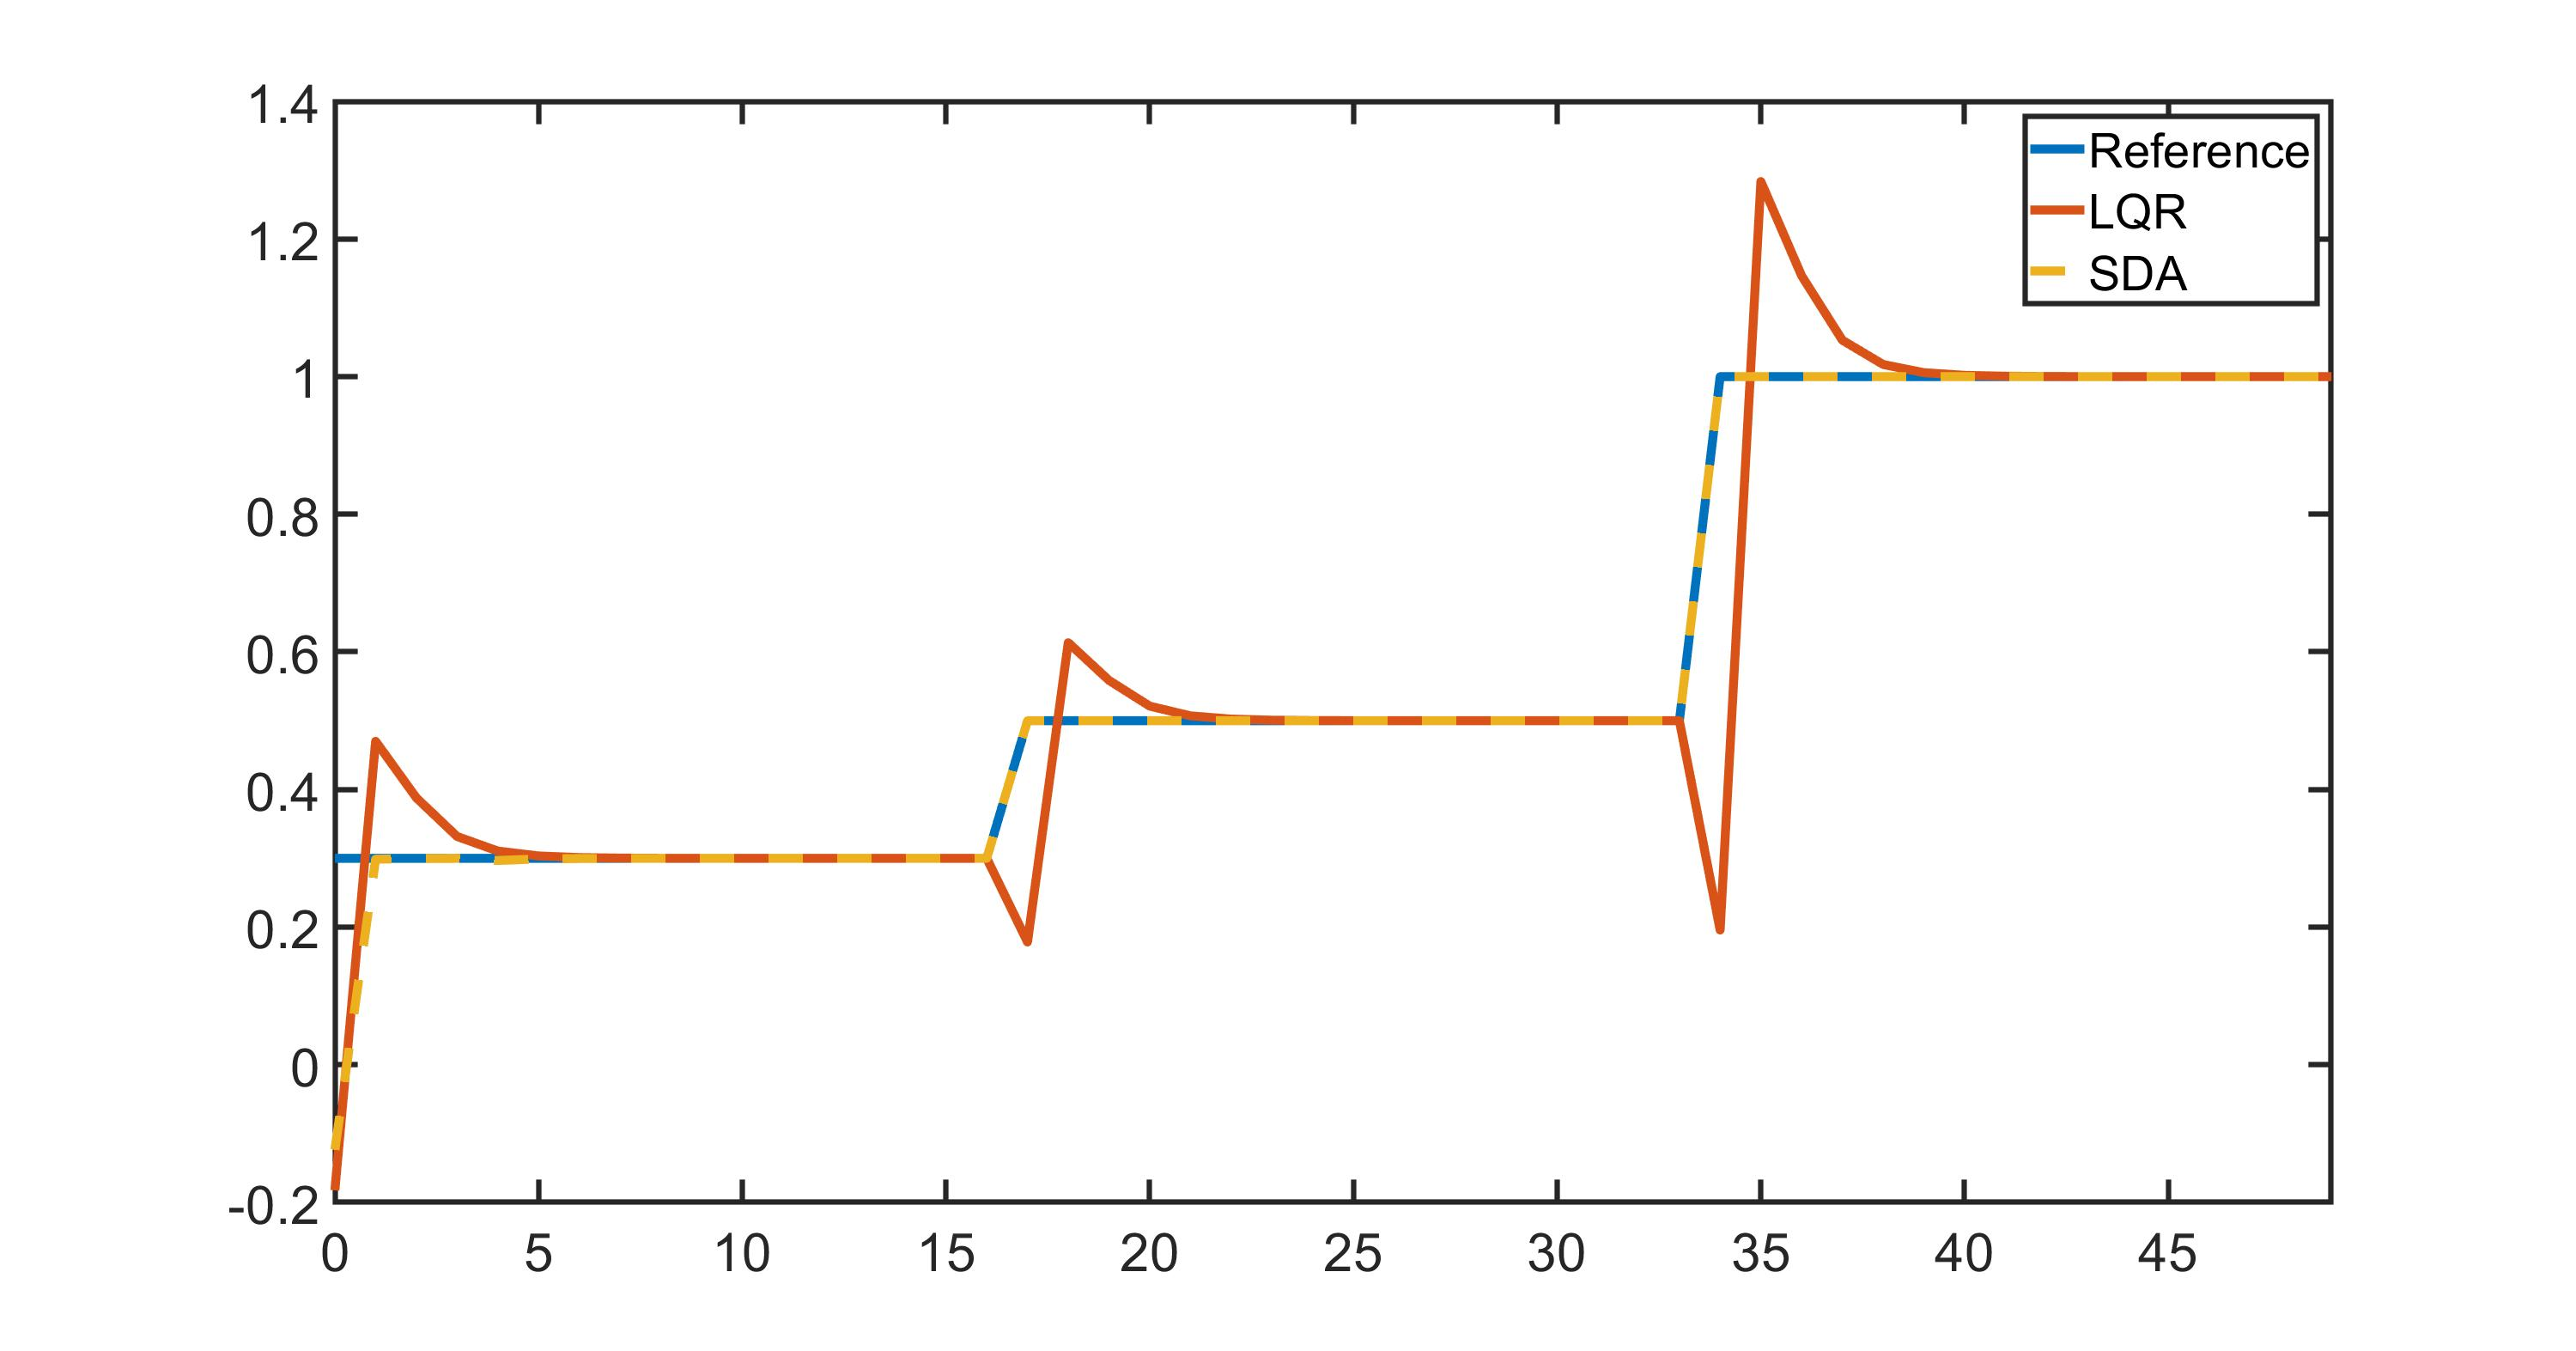
\includegraphics[width=\textwidth]{fig/Ex1_SDA.jpg}
	\caption{Reference signal tracking with LQR and SDA for the system \eqref{eq:ILC:Sys_ex1}}
	\label{img:ILC:Ex1_SDA}
\end{figure}

By choosing the weight $R$ we can regulate the control action. As we limit the possible input signals, it also leads to a rapid convergence. For example, for $R = I$ we need 8124 iterations, while with 
\begin{align}
R = \diag \begin{pmatrix}
1& 1 & 1 & 1 & 0.1 & \dots & 0.1
\end{pmatrix}
\end{align}
only 2569 trials are required. 

\end{exam}


\subsection{Suppression of eigenvalues} 

In the previous algorithms we assumed the learning matrix $K$ to be constant for all iterations.
We can presume another controller structure and set variable $K_k$ for $k\geq 0$. 

The simplest modification way is to set an iteration varying gain $\beta$ for each step: $K_k = \beta_k K_0$, $k\geq 0$ for a fixed matrix $K_0$. 

Let us consider the eigenvalues of the matrix $GG^\star$ and choose the gains $\beta_k$, $k \geq 0$ according to them. 

\begin{theo}
	Assume, that the matrix $GG^\star$ has $q+1$ non-zero ordered eigenvalues $\lambda_0, \lambda_1, \dots ,  \lambda_q$. Set $\beta_k = \frac{1}{\lambda_k}$ for $k = 0, 1, \dots, \, q$ and consider the update law
	\begin{align}
	\label{eq:cl_var0}
	\begin{split}
	u_{k+1} &= u_k + \beta_k G^\star e_k, \\
	e _{k+1} &= (I - \beta_{k+1}  GG^\star) e_{k}  = \prod_{l = 0}^{k+1} (I - \beta_{l}  GG^\star) e_0, \; k\geq 0,\\
	u_0 &\in \R^{l (N+1)}.
	\end{split}
	\end{align}
	Then the error sequence $(e_k)_{k\geq 0}$ converges in a finite number of iterations.     
\end{theo}
\begin{proof} 
	Set $\t{N} := m(N+1) - 1$. With spectral theorem, there exists a basis of the eigenvectors $\{v_0, v_1, \dots, v_{\t N}\}$ with corresponding eigenvalues $\lambda_0, \lambda_1, \dots, \lambda_q, 0, \dots 0$. 
	Then we can write $e_0$ as 
	\begin{align}
	e_0 = \sum_{p = 0}^{\t N} \gamma_p v_p
	\end{align}
	with uniquely defined $\gamma_p \in \R$, $p = 0, 1, \dots, \t N$. 
	
	For $k \in \N$ it follows 
	\begin{align}
	e_k = \left(\prod_{j=0}^k(I - \beta_j G G^\star)\right)e_0 = \sum_{p = 0}^{\t N} \gamma_p \left(\prod_{j=0}^k (I - \beta_j \lambda_p I)\right)v_p.
	\end{align}
	
	For the first iteration the error becomes 
	\begin{align}
	e_1 = \sum_{p = 0}^{\t N} \gamma_p ( I - \beta_1 \lambda_p I) v_p = \sum_{p=1}^{\t N } \gamma_p ( I - \beta_1 \lambda_p I) v_p.
	\end{align}
	
	The component $v_0$ is eliminated from the error.
	Assuming, that for $k \geq 1$ the first $k$ components were eliminated, we get 
	\begin{align}
	e_{k+1} = \sum_{p = 0}^{\t N} \gamma_p \left(\prod_{j=0}^k (I - \beta_j \lambda_p I)\right)v_p = \sum_{p = k + 1}^{\t N} \gamma_p \left(\prod_{j = 0}^k (I - \beta_j \lambda_p I )\right),
	\end{align}
	and hence the first $k+1$ components $v_0, v_1, \dots, v_k$ are eliminated. 
	By induction, the iteration process terminates after, at most,  $m(N+1) - q - 1$ iterations, as all non-zero eigenvalues have been covered and hence all corresponding eigenvectors are eliminated.	
\end{proof}

Although this algorithm is conceptually interesting, it is not suitable for real-world problems.
One can see, that the small non-zero eigenvalues of $GG^\star$ will lead to very large values of $\beta_k$ and hence we get extremely large transient variations in error norm. 
%The model errors can make this problem intolerable when elimination of eigenvector components will not be achieved in any iteration and/ or may be re-introduced in later iterations. 

Also computing the eigenvalues can be numerically questionable. Moreover, to achieve the monotonic convergence we need to consider only the eigenvalues $\lambda > \frac{1}{2}\lama(H)$.
If our model is inaccurate, and some eigenvalues are uncertain, it has directly impact on the algorithm result. 

That all makes this algorithm not solid. Still, we can use the idea to apply the eigenvalues of $G G^{\star}$ -- but not directly. We can try to ''pick'' the compatible eigenvalues.
\begin{alg}
	Choose a finite number $N_p + 1$ of points $p_0, p_1, \dots$ spread over the half-open interval $(\frac{1}{2}\lama(H), \lama(H)]$. 
	The Gradient Algorithm with Suppression of Eigenvalues (SoE Algorithm) is defined via choosing of the iteration-depending control law  $K_k = \beta_k G^\star e_k$, where 
	\begin{align}
	\begin{split}
	\beta_k &= \frac{1}{p_k} \text{ for } k = 0 , 1, \dots , N_p,\\
	\beta_k &= \beta  \text{ for } k > N_p,
	\end{split}
	\end{align}
	with $\beta \in (0, \frac{2}{\sigma_{\max}^2})$.
	
	Then the input update law becomes 
	\begin{align}
		u_{k+1} &= u_k + \beta_k G^\star e_k, \; k\geq 0,\\
		u_0 &\in \R^{l(N+1)}, 
	\end{align}
	and error evolution results in 
	\begin{align}
	\begin{split}
	e _{k} &= \left[\prod_{l = 0}^k (I - \beta_l  GG^\star) \right] e_{0}, \;  k = 0 , 1, \dots , N_p,\\
	e _{k} &=  (I - \beta GG^\star)^{k - N_p} e_{N_p}, \;  k > N_p, \\
	\end{split}
	\end{align}	
\end{alg}

This algorithm has the same convergence properties as Algorithm \ref{alg:SDA}, but potentially better convergence rates due to the eigenvalue suppression. Intuitively, the approach will increase the convergence speed in the first $N_p + 1$ iterations, if $N_p$ is large enough for good approximation of the interval $(\frac{1}{2} \lama(H), \lama(H)]$.

\begin{exam}
	We apply the SoE Algorithm on the system \eqref{eq:ILC:Sys_ex1} with weights $Q = I$, $R = I$.  
	The error evolution we get is illustrated in Figure \ref{img:ILC:Ex1_SDAvsSoE}.
	
	The new algorithms needs only 121 iterations, while the not adjusted SDA 730 trials are necessary. Indeed, for 31 of 51 eigenvalues $\lambda$ of $G G^\star$ holds 
	\begin{align}
	\lambda > \frac{1}{2}\lama(H) = 461.5 \, .
	\end{align}
	
	We can also see the influence of the weighting matrices on the convergence speed. 
	Since we do not need the better performance at the first time steps, we also need much less iterations. 
	   		
	\begin{figure}[ht]
		\centering
		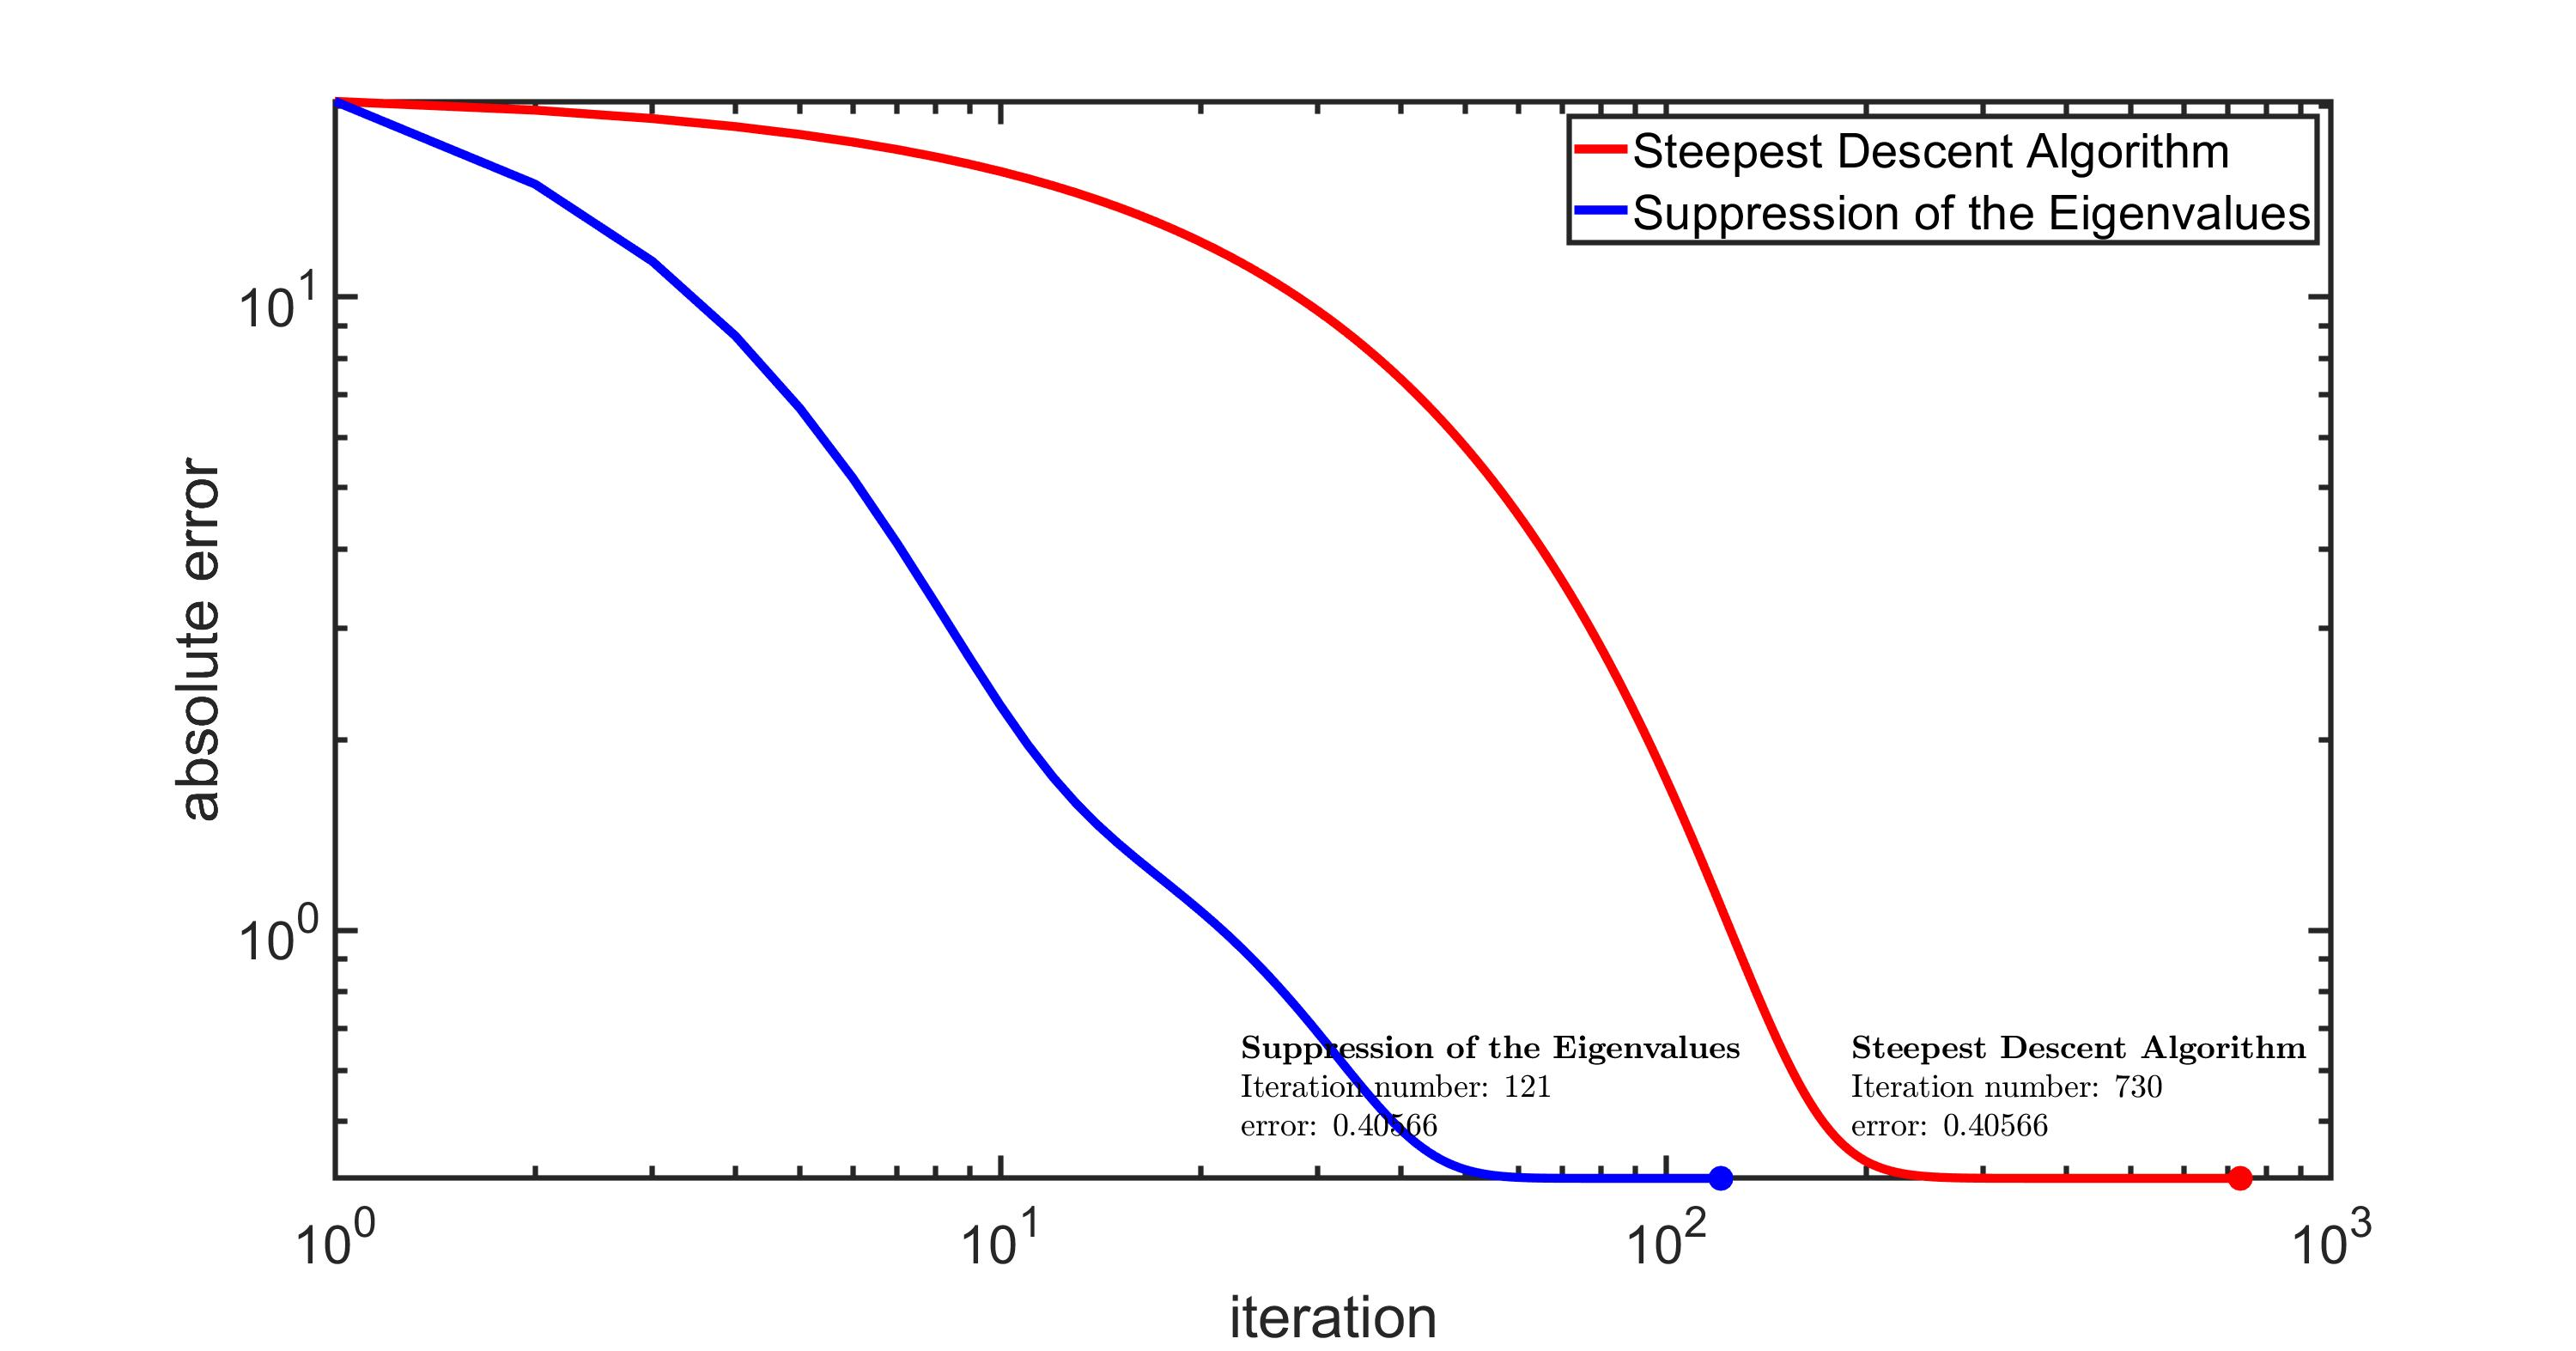
\includegraphics[width=\textwidth]{fig/Ex1_SDAvsSoE.jpg}
		\caption{Error evolution for SDA and SoE for system \eqref{eq:ILC:Sys_ex1}}
		\label{img:ILC:Ex1_SDAvsSoE}
	\end{figure}
	
\end{exam}

\section{Feedback Design}

With the previous algorithms we can achieve a better tracking for repetitively executed processes.  But they do not accent the special features of the model. For example, we can not manage the non-minimum-phase zeros, which can impact the convergence rate \cite{ILC}. 
If we consider the plant structure and construct a feedback controller, and then convert it into a steepest descent-like algorithm, we possibly can achieve better performance and robustness properties. 

Let us denote with $G(z)$ the transfer matrix in variable $z$ of the system $(A,B,C,D)$, and with $G$ the supervector matrix. 

More precisely, we consider a forward path compensator $K_c(z)$ in a unity negative feedback system for \eqref{eq:GP}. 
The design criteria for $K_c(z)$ include the closed-loop stability and the ability to track, albeit approximately, the reference signal $r$. With this compensator, depending on the model, we can remedy the plant properties such as oscillation, loop interaction, or the effects of non-minimum-phase zeros. 

We denote the complementary sensitivity of the resulting closed loop with $T(z)$ and its sensitivity with $S(z)$:
\begin{align}
T(z) = (I + G(z) K_c(z))^{-1}G(z) K_c(z) \text{ and } S(z)  = I - T(z) =  (I + G(z) K_c(z))^{-1}, 
\end{align}

and define the controller
\begin{align}
K_0(z) = K_c(z) S(z). 
\end{align}

Then the compensated Steepest Descent Algorithm is given as follows. 

\begin{alg}
	\label{alg: FBDesign}
	Write the transfer functions in supervector description as 
	$K_0$, $K_c$, $T$ and $S$. The compensated Steepest Descent Algorithm is  is characterized by choosing  $K = \beta K_0$, $\beta \in \R$. 
	The iterative law is given via 
	\begin{align}
	\label{eq:errFBDesign}
	\begin{split}
	u_{k+1} &= u_k + \beta K_0 T^* e_k, \\
	e_{k+1} &= (I- \beta T T^*) e_{k}, \; k\geq 0,\\
	u_0& \in \R^{l (N+1)}. 
	\end{split}	
	\end{align}
	Monotonic convergence to 
	\begin{align}
	\label{eq:FDErrLim} 
	e_\infty  = \lim_{k\to\infty} e_k = P_{\ker[T^*]}e_0,
	\end{align} 
	is guaranteed if
	\begin{align*}
	0 <\beta < \frac{2}{\lama(T T^*)}.
\end{align*}
$T^*$ stays here for conjugate transpose of the matrix $T$. 
\end{alg}
\begin{proof}
	The proof is identical to this in Algorithm \ref{alg:SDA} if consider the system 
	\begin{align}
	\t y = T\t u + \t d.
	\end{align}
\end{proof}

The effect of the operator $T T^*$ can be seen by considering the closed-loop relation 
\begin{align}
y = Tr.
\end{align}
We get a perfect tracking, if $T = I$, which is not achievable by feedback control. Still, we can assume a good tracking if $||T|| \approx 1$. 

Therefore if $K_c$ provides excellent feedback control of $G$, then rapid convergence could be attained with a choice of gain $\beta \approx 1$ \cite{ILC}. % if and the dominant frequency content of the reference $r$ lies in the bandwidth of the closed loop system $T$








\chapter{Robustness of the ILC Algorithms}
\label{ch:Robustness}
If our model is not precisely known, a chosen ILC algorithm might not provide the desired result. 
Therefore it is useful to consider how robust the algorithms are. 
In this thesis, we are going to consider the parametric uncertainty. That means, we do not know the true value of a real parameter (or the parameters) but know some range in which this parameter must lie. 

We can normalize such uncertainties without loss of generality, as any uncertainty $\delta \in [a,b] \subset \R$ can be expressed as 
\begin{align}
\label{eq:rob:del=del0+...}
\delta = \delta_0 + w \hat{\delta}
\end{align}
with $\hat{\delta} \in [-1,1]$, nominal value $\delta_0 \in \R$ and weight $w\in \R$. 

%Such uncertainties can be described as a set of the real diagonal matrices \cite{SchRC}. Each  matrix $\hat{\Delta}$ from this set can be  bounded
% with a matrix norm $|| \cdot ||$. With this norm, we can measure ''how much'' robust is our algorithm or system. Typically, one can bound this norm with 1, and put the scalings into the weights. {\color{red} Hier kommt vielleicht ein Beispiel, wie man das mit dem Rausziehen und den Weights macht}.
%

In order to guarantee the convergence of the algorithms despite such parametric uncertainties it is required that \eqref{eq:e_k}  stays stable for all possible parameter values.

Let us consider how the uncertainty looks like in the lifted system and deliberate over the method to solve the robustness issue.


%\begin{align}
%\hat{\Delf} = \{\hat{\Delta} = \begin{pmatrix}
%\delta_1 & & & \\
%&  \delta_2 & & \\
%& &  \ddots &  \\
%& & & \delta_\tau 
%\end{pmatrix}| \;\delta_i \in [-1,1] \text{ for } i = 1, 2, \dots, \tau\}
%\end{align}
%with $\tau$ of the fit dimension.



%For example, let us look at the system (A, B, C, D), with 
%\begin{align}
%A = \begin{pmatrix}
%-.5 + a & \\
%0       & 0 -.4 - a
%\end{pmatrix}, 
%B = \begin{pmatrix}
%1 \\ 1
%\end{pmatrix}, C = \begin{pmatrix}
%.1 & .2
%\end{pmatrix} \text{ and } 
%D = 1.
%\end{align}
%
%The uncertain parameter $a$ has the nominal value $\hat{a} = 1.5$ and variability $a \in [1.3, \; 1.8].








\section{Uncertain Lifted System} 

Let us consider a system \eqref{eq:Intro:GP} with uncertainty $\hat{\Delta} $ from the set 
\begin{align}
\label{eq:Delta_hat_set}
\hat{\Delf} =
\left\{\begin{array}{c|c}
\begin{pmatrix}
\delta_1 I_{p_1} & & &\\
& & \ddots &\\
& & &\delta_\tau I_{p_\tau}
\end{pmatrix} & \; \delta_l \in [-1,\;1], p_l \in \N \text{ for } l = 1, 2, \dots , \tau .
\end{array} \right\}.
\end{align}
$\tau \in \N$ is the number of the uncertain parameter.

Each uncertain system $\left[\begin{array}{c|c}
A & B \\\hline C &D
\end{array}\right]\left(\hat{\Delta}\right)$
we can rewrite as a feedback interconnection of the system 
$
\left[\begin{array}{c|c c}
A_1 & B_1 & B_2 \\\hline
C_1 & D_{11} & D_{12} \\
C_2 & D_{21} & D_{22}
\end{array}\right]
$
and $\hat{\Delta}$. 
Then the original system can be found as star product (also called linear fractional transformation or LFT)
\begin{align}
\left[\begin{array}{c|c}
A & B \\\hline C &D
\end{array}\right] = \hat{\Delta} \star \left[\begin{array}{c|c c}
A_1 & B_1 & B_2 \\\hline
C_1 & D_{11} & D_{12} \\
C_2 & D_{21} & D_{22}	
\end{array}\right]
\end{align}

We illustrate it in the Figure \ref{fig:Rob:LFR}. 
We speak here about the ''pulling out'' the uncertainty, or the \textit{linear fractional representation} (LFR). 


With LFR we rewrite the system \eqref{eq:Intro:GP} as 
\begin{align}
\label{eq:uncABCD}
\begin{split}
x(t+1) &= A_1 x(t) + B_1 u(t) + B_2 w(t), \\
y(t)   &= C_1x(t) + D_{11} u(t) + D_{12} w(t), \\
z(t)   &= C_2x(t) + D_{21} u(t) + D_{22}w(t),\\
w(t) &= \hat{\Delta} z(t),\\
x(0)& \in \R^{n}, t = 0,1,2, \dots, N, 
\end{split}
\end{align}
with error $e(\cdot) = r(\cdot) - y(\cdot)$. 


\begin{figure}
	\begin{center}
		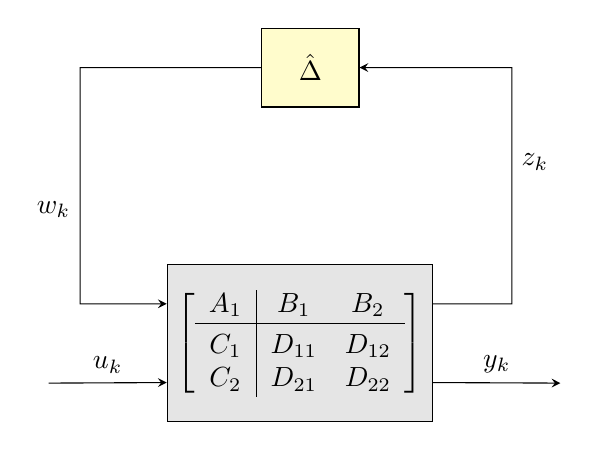
\begin{tikzpicture}[>=stealth]
		%coordinates
		\coordinate (orig)   at (0,0);
		
		\coordinate (AroneA) at (-3,1.5);
		\coordinate (ArtwoA) at (5,.5);
		\coordinate (ArthrA) at (-1.5,.5);
		\coordinate (LLA)    at (0,0);
		\coordinate (LLD)    at (1.2,4);
		
		%nodes
		\node[draw, minimum width=2cm, minimum height=2cm, anchor=south west, align=center, fill = gray!20] (A) at (LLA) {$\left[\begin{array}{c|c c}
			A_1 & B_1 & B_2 \\\hline C_1 & D_{11} & D_{12} \\ C_2 & D_{21} & D_{22}
			\end{array}\right]$};
		\node[draw, minimum width=1.2cm, minimum height=1cm, anchor=south west, text width=1cm, align=center ,fill = yellow!20] (D) at (LLD) {$\hat{\Delta}$};
		
		\draw[->] (ArthrA) -- node[above]{$u_k$} ($(A.180) + (0,-1/2)$);
		\draw[->]  ($(A.east) - (0,.5)$) -- node[above]{$y_{k}$}(ArtwoA);
		
		\draw[->] ($(A.0) + (0,1/2)$) -| ++ (1,1.5) -- node[right, pos=0.2]{$z_k$}++ (0,1.5) -- ($(D.east)$);		
		\draw[->] ($(D.west)$) -| ++ (-2.3,-1.5) -- node[left, pos=0.2]{$w_k$} ++ (0,-1.5) -- ($(A.180) + (0,1/2)$);
		\end{tikzpicture}
		
	\end{center}
	\caption{Uncertain system as feedback interconnection of LFR and the uncertainty $\hat{\Delta}$} \label{fig:Rob:LFR}
\end{figure}
The corresponding lifted  system has the form 
\begin{align}
y &= G_1 u + G_2 w + d_1, \\
z &= G_3 u + G_4 w + d_2, \\
e &= r - y,\\
w &= \Delta z,
\end{align}
with the matrices
\begin{align}
G_1 &= \nonumber \\
&=  \begin{pmatrix}
	D_{11} & 0 & \cdots & 0 & 0 & 0 \\
	C_1B_1 & D_{11} & \cdots & 0 & 0 & 0\\
	C_1A_1B_1 & C_1B_1 & \cdots & 0 & 0 & 0\\
	\vdots & \vdots & \ddots & \vdots  & \vdots & \vdots \\
	C_1A_1^{N-2} B_1 & C_1A_1^{N-3} B_1 &\dots &C_1B_1 & D_{11}& 0\\
	C_1A_1^{N-1} B_1 & C_1A_1^{N-2} B_1 &\dots &C_1A_1B_1 & C_1B_1& D_{11}\\
\end{pmatrix},
\end{align}
\begin{align}G_2 & = \nonumber\\
&= \begin{pmatrix}
D_{12} & 0 & \cdots & 0 & 0 & 0 \\
C_1B_2 & D_{12} & \cdots & 0 & 0 & 0\\
C_1A_1B_2 & C_1B_2 & \cdots & 0 & 0 & 0\\
\vdots & \vdots & \ddots & \vdots  & \vdots & \vdots \\
C_1A_1^{N-2} B_2 & C_1A_1^{N-3} B_2 &\dots &C_1B_2 & D_{12}& 0\\
C_1A_1^{N-1} B_2 & C_1A_1^{N-2} B_2 &\dots &C_1A_1B_2 & C_1B_2& D_{12}\\
\end{pmatrix},
\end{align}
\begin{align}
G_3 & = \nonumber\\
&= \begin{pmatrix}
D_{21} & 0 & \cdots & 0 & 0 & 0 \\
C_2B_1 & D_{21} & \cdots & 0 & 0 & 0\\
C_2A_1B_1 & C_2B_1 & \cdots & 0 & 0 & 0\\
\vdots & \vdots & \ddots & \vdots  & \vdots & \vdots \\
C_2A_1^{N-2} B_1 & C_2A_1^{N-3} B_1 &\dots &C_2B_1 & D_{21}& 0\\
C_2A_1^{N-1} B_1 & C_2A_1^{N-2} B_1 &\dots &C_2A_1B_1 & C_2B_1& D_{21}\\
\end{pmatrix},
\end{align}
\begin{align}
G_4 & = \nonumber\\
&= \begin{pmatrix}
D_{22} & 0 & \cdots & 0 & 0 & 0 \\
C_2B_2 & D_{22} & \cdots & 0 & 0 & 0\\
C_2A_1B_2 & C_2B_2 & \cdots & 0 & 0 & 0\\
\vdots & \vdots & \ddots & \vdots  & \vdots & \vdots \\
C_2A_1^{N-2} B_2 & C_2A_1^{N-3} B_2 &\dots &C_2B_2 & D_{22}& 0\\
C_2A_1^{N-1} B_2 & C_2A_1^{N-2} B_2 &\dots &C_2A_1B_2 & C_2B_2& D_{22}\\
\end{pmatrix},
\end{align}
and vectors 
\begin{align}
d_1 = \begin{pmatrix}
C_1 x_0 \\ C_1A_1 x_0 \\ C_1A_1^2 x_0 \\ \vdots \\ C_1A_1^Nx_0
\end{pmatrix},
\end{align}
\begin{align}
d_2 = \begin{pmatrix}
C_2 x_0 \\ C_2A_1 x_0 \\ C_2A_1^2 x_0 \\ \vdots \\ C_2A_1^Nx_0
\end{pmatrix}.
\end{align}
$\Delta$ is here a block diagonal matrix 
\begin{align}
\Delta = \diag(\underbrace{\hat{\Delta}, \hat{\Delta}, \dots, \hat{\Delta}}_{(N+1) \text{ times}})
\end{align}
and we define 
\begin{align}
\Delf = \{\diag(\hat{\Delta}, \hat{\Delta}, \dots, \hat{\Delta})| \; \hat{\Delta}\in \hat{\Delf}\}.
\end{align}




Using LFT, we get 
\begin{align}
\label{eq:rob:y = G(Delta) + d(Delta)}
y&= G(\Delta)u + d(\Delta) := \left[G_1 + G_2 \Delta (I - G_4\Delta)^{-1}G_3\right] u + \left[G_2 \Delta (I - G_4\Delta)^{-1} d_2 + d_1\right], 
\end{align}
while the inverse of the matrix $(I - G_4\Delta)$ is assumed to exist. It is always the case if the norm of the matrix $G_4$ is (strictly) bounded by 1 \cite{SchRC}.



%TODOO: A -> A_1

With ILC algorithms we get the input update rule
\begin{align}
u_{k+1} = u_k + Ke_k,
\end{align}
and hence 
\begin{align}
\label{eq:LekUnc}
e_{k+1} = L(\Delta)e_k = (I - G(\Delta)K) e_k.
\end{align}
If we pull out the uncertainty from $L(\Delta)$, we get 
%
%From our algorithms, we get the matrix $L$, which depends on the model and hence it depends on
% the given uncertainty. 
%With the methods from \cite{SchRC} we can pull out the uncertainty, and get the controlled system 
\begin{align}
\begin{split}
\left(\begin{array}{c}
e_{k+1} \\ \hline z_k
\end{array}\right) &= 
\left(\begin{array}{c| c}
\c{A} & \c{B} \\
\hline
\c{C} & \c{D}
\end{array}\right) \left(\begin{array}{c}
e_{k}  \\\hline w_k
\end{array}\right):= 
\left(\begin{array}{c|c}
I - G_1 & -G_2 \\
\hline
G_3 K & G_4
\end{array}\right)
\left(\begin{array}{c}
e_{k}  \\\hline w_k
\end{array}\right),\\
w_k &= \Delta z_k,
\end{split}
\end{align}
with the uncertain system defined through the uncertain matrix 
\begin{align}
\label{eq: LstarDelta}
L(\Delta) = \Delta \star \left(\begin{array}{c| c}
\c{A} & \c{B} \\
\hline
\c{C} & \c{D}
\end{array}\right) = \c{A} + \c{B} \Delta (I - \c{D}\Delta)^{-1}\c{C}. 
\end{align}
 We are interested in stability ensuring for the system \eqref{eq:LekUnc}. 
 
 The most intuitive way is to ensure $||L(\Delta)||<1$ for all uncertainties $\Delta \in \Delf$.
 %, since this implies 
% \begin{align}
% ||e_{k+1}|| = 	||L(\Delta)^ke_0|| \leq ||L(\Delta)||^k ||e_0|| \to 0 \text{ for } k \to \infty||.
% \end{align}
However, this criteria might be too restrictive. We illustrate it on the following example. 

\begin{exam}
	\label{exp:rob:bad_example}
Let us consider the system 
\begin{align}
e_{k+1}  = L(\alpha) e_k = \begin{pmatrix}
.1 & \alpha \\ 0 & .1
\end{pmatrix}e_k
\end{align}
with an  uncertain parameter $\alpha \in \R$.
Then the norm $||L(\alpha)||$ is proportional to $|\alpha|$.

For example, with the spectral norm, we can ensure stability only for $|\alpha|<1$. 


On the other hand, one can directly see, that the system is stable for all $\alpha \in \R$, since the eigenvalues of the matrix equal $.1$. 	
\end{exam}

This example motivates to devise another method for ensuring the stability of  such uncertain systems. 
We can reach much more elegant results by considering stability using Lyapunov techniques. 

 

\section{Robustness Proof with LMI}

First, let us consider the uncertainty $\Delta$ without taking into account its structure. 
Using the Lyapunov Linear Matrix Inequality (LMI) we formulate the following Theorem. 
\begin{theo}
	\label{thm:Lyap}
	Suppose that there exists some positive definite matrix $X$ satisfying 
	\begin{align}
	\label{eq:Lyap}
	\begin{pmatrix}
	I \\ L(\Delta) 
	\end{pmatrix}^T
	\begin{pmatrix}
	-X & 0 \\ 0 & X
	\end{pmatrix}
	\begin{pmatrix}
	I \\ L(\Delta) 
	\end{pmatrix} = L(\Delta)X L(\Delta) - X \preceq 0 \text{ for all } \Delta \in \Delf.
	\end{align}
	Then the discrete dynamical system \eqref{eq:LekUnc} 
	is stable for all $\Delta \in \Delf$ and for all $e_0 \in \R^{m ( N+1)}$.
	It is asymptotically stable if the inequality is strict. 
\end{theo}
\begin{proof}
	First, let us prove the Theorem for the strict LMI. Then, we can find some $\gamma \in (0,1)$, such that
	\begin{align}
	\label{eq:proof0}
	\begin{pmatrix}
	I \\ L(\Delta)
	\end{pmatrix}
	\begin{pmatrix}
	-\gamma X & 0 \\ 0 & X
	\end{pmatrix}
	\begin{pmatrix}
	I \\ L(\Delta)
	\end{pmatrix} = L(\Delta)^T X L(\Delta) - \gamma X \prec 0 \text{ for all } \Delta \in \Delf.
	\end{align}	
	

	Moreover, since $X \succ 0$, there exist some $\alpha, \beta > 0$, such that 
	\begin{align}
	\label{eq:proof1}
	\alpha I \prec X \prec \beta I.
	\end{align}
	
	Set $\eta_k := e_k^T X e_k$. Then we have
	\begin{align}
	\label{eq:proof2}
	\eta_{k+1} = e_{k+1}^T X e_{k+1} = e_k^T L(\Delta)^T X L(\Delta) e_k \leq \gamma e_k X e_k = \gamma \eta_k \text{ for all } k\geq 0.
	\end{align}
    From \eqref{eq:proof1} we get
	\begin{align}
	\alpha || e_k ||^2 \leq \eta_k \leq \beta ||e_k||^2 \text{ for all } k\geq 0,
	\end{align}
	and with \eqref{eq:proof2} it follows
	\begin{align}
	\label{eq:proof3}
	||e_k||^2 \leq \frac{1}{\alpha}\eta_k \leq \frac{\gamma^k}{\alpha}\eta(0) \leq \frac{\beta}{\alpha} \gamma^k ||e_0||^2. 
	\end{align}
	
	
	Since $\gamma \in (0,\;1)$, $||e_k||^2 \to 0$ for $k \to \infty$, and taking the square root yields the proof. 
	
	For not the strict case, we set in \eqref{eq:proof2} and \eqref{eq:proof3} $\gamma = 1$, and replace in \eqref{eq:proof0} ''$\prec$'' with ''$\preceq$''. Then $||e_k||^2$ (and hence $||e_k||$) is bounded over all $k\geq 0$ and hence the system \eqref{eq:LekUnc} is stable. 
	
\end{proof}

In this Theorem, we still have the uncertainty in our LMI problem. 
To get rid of it, we fix the matrix $X\succ 0$ and try to find a multiplier $P = P^T$, which fulfills 
\begin{align}
	\label{eq:PDelta}
	\begin{pmatrix}
		I \\ \Delta
	\end{pmatrix}^T 
	P
	\begin{pmatrix}
		I \\ \Delta
	\end{pmatrix} \succeq 0,
\end{align}

and, additionally,
	\begin{align}
	\label{eq:strangeMatrix}
	\begin{pmatrix}
		I & 0 \\ \c{A} &  \c{B}
	\end{pmatrix}^T\begin{pmatrix}
		-X & 0 \\ 0 & X
	\end{pmatrix} 
	\begin{pmatrix}
		I & 0 \\ \c{A} &  \c{B}
	\end{pmatrix} + 
	\begin{pmatrix}
		\c{C} & \c{D} \\ 0 & I
	\end{pmatrix}^T
	P
	\begin{pmatrix}
		\c{C} & \c{D} \\ 0 & I
	\end{pmatrix} \preceq 0.
\end{align}

If we can find such a matrix $P$, the stability of the system \eqref{eq:LekUnc} can be proven. 

We formulate it as a Theorem. 

\begin{theo}
	\label{thm:stabViaP}
	Let $\mathbb{P}$ be a subset of the symmetric matrices, and $X \succ 0 $ be fixed.
	Then the system \eqref{eq:LekUnc} is stable if there exists a matrix $P = P^T \in \mathbb{P}$, such that \eqref{eq:PDelta} and \eqref{eq:strangeMatrix} are fulfilled. 
	If the inequality \eqref{eq:strangeMatrix} is strict, the system becomes asymptotic stable. 
\end{theo}

\begin{proof}	
	Let $P = P^T \in \mathbb{P}$ be some matrix, which fulfills the relations \eqref{eq:PDelta} and \eqref{eq:strangeMatrix}.
	
	We multiply \eqref{eq:strangeMatrix} with 
	\begin{align}
		H = \begin{pmatrix}
			I \\ \Delta ( I - \c{D} \Delta)^{-1}C
		\end{pmatrix}
	\end{align}	
right and its transpose left. Then the first term results in 
\begin{align}
%\begin{split}
%&	\begin{pmatrix}
%I \\ \Delta ( I - \c{D} \Delta)^{-1}C
%\end{pmatrix}^T 
H^T
\begin{pmatrix}
I & 0 \\ \c{A} &  \c{B}
\end{pmatrix}^T
\begin{pmatrix}
-X & 0 \\ 0 & X
\end{pmatrix} 
\begin{pmatrix}
I & 0 \\ \c{A} &  \c{B}
\end{pmatrix} H 
%\\= & -X + \c{A}^T X \c{A} + \c{A}^T X \c{B} \Delta(I - \Delta\c{D})^{-1} \c{C} + \c{C}^T(I - \Delta\c{D})^{-T}\c{B}^T X \c{B} (I - \Delta\c{D})^{-1}\c{C} \\
= L(\Delta)^T X L(\Delta) - X.
\end{align}
	
	Hence, if we can prove that the second term multiplied with $H$ right and its transpose left is positive semi-definite, this matrix $P$ will ensure the monotonic convergence of the algorithms. Multiplying $H$ yields 
	\begin{align*}
	&H^T\begin{pmatrix}
	\c{C} & \c{D} \\ 0 & I
	\end{pmatrix}^T
	P
	\begin{pmatrix}
	\c{C} & \c{D} \\ 0 & I
	\end{pmatrix} H  = 
	(I - \Delta \c{D})^{-T} \underbrace{\begin{pmatrix}
		I \\ \Delta 
		\end{pmatrix}^T P
		\begin{pmatrix}
		I \\ \Delta 
		\end{pmatrix}}_{\succeq 0}(I - \Delta \c{D})
	\succeq 0,
	\end{align*}
	what proofs the first statement. 
	If the inequality \eqref{eq:strangeMatrix} is strict, the LMI \eqref{eq:Lyap} is also strict and we achieve the asymptotic stability. 
\end{proof}



So, the robustness issue can be reduced to a certain LMI over a multiplier set $\mathbb{P}$. 

The choosing of the set $\mathbb{P}$ is here the cornerstone. It must be large enough, to be able to find such multiplier $P$, if the system is stable, but also adequate small, such that the searching action is not too costly. 
 
Let us begin with a single uncertain parameter $\delta$. Then the uncertainty $\Delta = \delta I$ with $\delta \in [-1,\; 1]$. 
A possible choice for a multiplier set is 
\begin{align}
\mathbb{P}= \{ \begin{pmatrix}
S & R \\ R^T & -S
\end{pmatrix}| \; S \succeq 0 , \; R + R^T = 0\}.
\end{align}
There is 
\begin{align}
\begin{pmatrix}
I \\ \delta I
\end{pmatrix}^T 
\begin{pmatrix}
S & R \\ R^T & -S
\end{pmatrix}
\begin{pmatrix}
I \\ \delta I
\end{pmatrix} = \underbrace{(1 - \delta^2 )}_{\geq 0}S + \delta\underbrace{(R + R^T)}_{=0} \succeq 0,
\end{align}
and hence the requirements on the set $\mathbb{P}$ for the Theorem \eqref{thm:stabViaP} are fulfilled. 

For $\tau \in \N$ uncertain real parameters the uncertainty has the form 
\begin{align}\Delta= \diag(\underbrace{\hat{\Delta}_\tau, \hat{\Delta}_\tau, \dots, \hat{\Delta}_\tau}_{(N+1) \text{ times }})\end{align}
with
\begin{align}
\hat{\Delta}_\tau = \begin{pmatrix}
\delta_1 I_{p_1}& & & \\
& \delta_2 I_{p_2} & & \\
& & \ddots & \\
& & & \delta_\tau I_{p_\tau}
\end{pmatrix}.
\end{align}

We choose a permutation matrix $\c{P}$, such that 
\begin{align}
\label{eq:rob:PDelta}
\Delta_\text{perm}= 
\c{P} \Delta =
\begin{pmatrix}
\delta_1 I_{(p_1\cdot N)} & & &\\
& \delta_2 I_{(p_2\cdot N)} & & \\
& & \ddots & \\
& & & \delta_\tau I_{(p_\tau \cdot N)}
\end{pmatrix}.
\end{align}

If we choose the multiplier set 
\begin{align}
\mathbb{P}_\tau =\left\{\begin{array}{c|c}
  \begin{pmatrix}
  I_{\tau(N+1)} \\ \c{P}
  \end{pmatrix}^T  
  \begin{pmatrix}
S & R \\ R^T & -S
\end{pmatrix}
\begin{pmatrix}
I_{\tau (N+1)} \\ \c{P}
\end{pmatrix}
& \; \begin{array}{c} S = \diag(S_1, S_2, \dots, S_\tau)\succeq 0,\\ R = \diag(R_1, R_2, \dots, R_\tau), R + R^T = 0\end{array} \end{array}
\right\},
\end{align}
then for $P_\tau \in \mathbb{P}_\tau$,  the following relation is satisfied
\begin{align}
\begin{pmatrix}
I \\ \Delta
\end{pmatrix}^T
P_\tau
\begin{pmatrix}
I \\ \Delta
\end{pmatrix}
&=
\begin{pmatrix}
I \\ \Delta_\text{perm}
\end{pmatrix}^T
\begin{pmatrix}
S & R \\ R^T & -S
\end{pmatrix}
\begin{pmatrix}
I \\ \Delta_\text{perm}
\end{pmatrix}\\
&= 
\begin{pmatrix}
(1 - \delta_1^2)S_1 & & &\\
& (1 - \delta_2^2) S_2 & & \\
& & \ddots & \\
& & & (1- \delta_\tau^2) S_\tau
\end{pmatrix}.
\end{align}





%
%the convergence properties of the algorithm are not impacted: $G(\Delta)$ in \eqref{eq:rob:y = G(Delta) + d(Delta)} can be rewritten as 
%\begin{align}
%G(\Delta) &= G_1 + G_2  \c{P}^T \c{P} \Delta(I - G_4 \c{P}^T \c{P} \Delta)^{-1}G_3 \\
%&= 
%(\c{P}\Delta) \star \left[\left(\begin{array}{c | c}
%G_1 & G_2 \\ \hline
%G_3 & G_4
%\end{array}\right)\begin{pmatrix}
%I & \\ & \c{P}^T
%\end{pmatrix}\right],
%\end{align}
%and the uncertain vector $d(\Delta)$ as 
%\begin{align}
%d(\Delta) &= G_2\c{P}^T\c{P} \Delta (I - G_4\c{P}^T\c{P}\Delta)^{-1} d_2 + d_1 \\
%&= 
%(\c{P}\Delta) \star \left[\left(\begin{array}{c | c}
%d_1 & G_2  \\ \hline
%d_2 & G_4 
%\end{array}\right)\begin{pmatrix}
%I & \\ & \c{P}^T
%\end{pmatrix}\right].
%\end{align}
%
%Hence we can use the structure as in \eqref{eq:rob:PDelta} without loss of generality.
%The multiplier set can be chosen as 
%\begin{align}
%\mathbb{P}_\tau =\left\{\begin{array}{c|c}
%\begin{pmatrix}
%S & R \\ R^T & -S
%\end{pmatrix}
%& \; \begin{array}{c} S = \diag(S_1, S_2, \dots, S_\tau)\succeq 0,\\ R = \diag(R_1, R_2, \dots, R_\tau), R + R^T = 0\end{array} \end{array}
%\right\}.
%\end{align}
%
%For $P_\tau \in \mathbb{P}_\tau$
%\begin{align}
%\begin{pmatrix}
%I \\ \Delta_\text{perm}
%\end{pmatrix}^T
%P_\tau
%\begin{pmatrix}
%I \\ \Delta_\text{perm}
%\end{pmatrix}
%= 
%\begin{pmatrix}
%(1 - \delta_1^2)S_1 & & &\\
%& (1 - \delta_2^2) S_2 & & \\
%& & \ddots & \\
%& & & (1- \delta_\tau^2) S_\tau
%\end{pmatrix}.
%\end{align}



Go back to Example \ref{exp:rob:bad_example}. 
Let $\alpha \in [0,2]$ be an uncertainty with the nomimal value $\alpha_0 = 1$.
With linear fractional transformation the system 
\begin{align}
e_{k+1} = \begin{pmatrix}
.1 & \alpha \\ 0 &.1
\end{pmatrix}e_k
\end{align}
results in 
\begin{align}
\begin{pmatrix}
e_{k+1} \\ z_k
\end{pmatrix} = 
\begin{pmatrix}
0 & 0 & 1 \\
1 & 0.1 & 1 \\
0 & 0 & 0.1
\end{pmatrix} \begin{pmatrix}
e_k \\ w
\end{pmatrix}. 
\end{align}
With the choice 
\begin{align}
X = \diag(2, 0.5)
\end{align}
we can compute with MATLAB the solution 
\begin{align}
P = \diag(4.61, -4.61), 
\end{align}
which renders the eigenvalues of the left side term in the relation \eqref{eq:strangeMatrix} to 
\begin{align}
\lambda_1 = -2.35, \; \lambda_2 = -1.21 \text{ and } \lambda_3 = -0.488.
\end{align}
Hence, according to the Theorem \ref{thm:stabViaP}, the system is stable for all $\alpha \in [0,2]$. 

\begin{exam}
	\label{ex:Rob:robvsN}
	In Chapter \ref{ch:ILCAlg} we said, that the choice of $\beta$ might impact the robustness properties of the Inverse Model Algorithms.
	Let us illustrate it on the system \eqref{eq:ILC:Sys_ex1}, but with uncertain parameter $a \in [\underline{a}, \; \overline{a}]$ and nominal value $a_0 = 4$: 
	\begin{align}
	A = \begin{pmatrix}
	2 & 1 \\  a & 3
	\end{pmatrix}
	\end{align}
			
	For $N = 23$ and $\beta = .1$ our system still stays robust for $\overline a = - \underline a = 2$. If we set $\beta = .4$, we can not ensure the robustness using Theorem \ref{thm:stabViaP} even for $\overline a = - \underline a = .1$. 
	
	However, the ability to find the adequate matrices $X$ and $P$ depends on the time horizon $N$. 
	For $N = 20$, we get a much more robust system, for which the stability can be proven for $\overline a = - \underline a = 5$. 
\end{exam}


	

	
	
	
	

	

%
%
%
%
%
%
%
%
%
%
%
%
%
%
%
%
%
%
%
% which gets us the matrix $L$. Since the matrix $L$ depends on the model we have, it also depends upon the uncertainty. 
%This uncertainty we assume to be $\Delta$, 
%
%We can pull out the uncertainty with the methods from \cite{RC}, and get 
%
% 
%Let us assume, that some parameter in the model is not exactly known. That means, we have some uncertainty which depends on $\delta \in [-1,
%\,1]$ \cite{SchRC}:
%\begin{align}
%\Delta = \Delta(\delta) = \delta I, \; \delta \in [-1, \, 1].
%\end{align}
%
%With the methods described in \cite{SchRC} let us pull out the uncertainty from $L$. Then the performance and uncertainty channel can be written as 
%\begin{align}
%\left[\begin{array}{c}
%e_{k+1} \\ \hline z_k
%\end{array}\right] &= 
%\left[\begin{array}{c| c}
%\c{A} & \c{B} \\
%\hline
%\c{C} & \c{D}
%\end{array}\right]
%\left[\begin{array}{c}
%e_{k}  \\\hline w_k
%\end{array}\right],\\
%w_k &= \delta z_k.
%\end{align}
%
%and $L$ is given via star product
%\begin{align}
%\label{eq: LstarDelta}
%L(\delta) = \delta I \star \left[\begin{array}{c| c}
%\c{A} & \c{B} \\
%\hline
%\c{C} & \c{D}
%\end{array}\right] = \c{A} + \c{B} \delta (I - \c{D}\delta)^{-1}\c{C}. 
%\end{align}
%
%We are interested in monotonic convergence of the algorithms in spite of the uncertainty $\Delta$. That means, we want to ensure the stability of the system $e_{k+1} = L e_k$. 
%This is possible using the following Theorem: 
%
%
%
%The previous Theorem is true for any structured uncertainty $\Delta$. 
%
%
%
%
%
%
%
%
%
%As we have seen before, it is not always possible to achieve perfect convergence. 
%The next Theorem provide a method to check, whether the chosen controller for \eqref{eq:stability} renders the system stable. We consider some uncertainty $\Delta$ from a compact set $\Delf$. 
%\begin{theo}
%	Suppose that there exists some positive definite matrix $X$ satisfying 
%	\begin{align}
%	\begin{pmatrix}
%	I \\ L(\Delta) 
%	\end{pmatrix}^T
%	\begin{pmatrix}
%	-X & 0 \\ 0 & X
%	\end{pmatrix}
%	\begin{pmatrix}
%	I \\ L(\Delta) 
%	\end{pmatrix} = L(\Delta)X L(\Delta) - X \preceq 0 \text{ for all } \Delta \in \Delf.
%	\end{align}
%	Then the discrete dynamical system 
%	\begin{align}
%	e_{k+1} = L(\Delta) e_k, \; k\geq 0
%	\end{align}
%	is stable for all $\Delta \in \Delf$ and for all $e_0 \in \R^{m ( N+1)}$.
%\end{theo}
%\begin{proof}
%	Since $X \succ 0$, there exist some $\alpha, \beta > 0$, such that 
%	\begin{align}
%	\alpha I \prec X \prec \beta I.
%	\end{align}
%	
%	Set $\eta_k := e_k^T X e_k$. Then 
%	\begin{align}
%	e_{k+1} = e_{k+1}^T X e_{k+1} = e_k^T L(\Delta)^T X L(\Delta) e_k \leq e_k X e_k = \eta_k \text{ for all } k\geq 0.
%	\end{align}
%	Hence
%	\begin{align}
%	\alpha || e_k ||^2 \leq \eta_k \leq \beta ||e_k||^2 \text{ for all } k\geq 0,
%	\end{align}
%	and it follows
%	\begin{align}
%	||e_k||^2 \leq \frac{1}{\alpha}\eta_k \leq \frac{1}{\alpha}\eta(0) \leq \frac{\beta}{\alpha} ||e_0||^2. 
%	\end{align}
%	Taking the square root yields the claim. 
%\end{proof}
%
%
%
%
%
%
%
%
%
% 
% 
% 
% 
% 
% 
%\section{Robust Zero Monotonic Convergence for Parametric Uncertainty}
%Let us assume, that some parameter in the model is not exactly known. That means, we have some uncertainty which depends on one parameter $\delta \in [-1,
%\,1]$ \cite{SchRC}:
%\begin{align}
%\Delta = \Delta(\delta) = \delta I, \; \delta \in [-1, \, 1], 
%\end{align}
%and since $L = L(\delta)$. 
%
%With the methods described in \cite{SchRC} let us pull out the uncertainty from $L$. Then the performance and uncertainty channel can be written as 
%\begin{align}
%\left[\begin{array}{c}
%e_{k+1} \\ \hline z_k
%\end{array}\right] &= 
%\left[\begin{array}{c| c}
%\c{A} & \c{B} \\
%\hline
%\c{C} & \c{D}
%\end{array}\right]
%\left[\begin{array}{c}
%e_{k}  \\\hline w_k
%\end{array}\right],\\
%w_k &= \Delta (\delta) z_k.
%\end{align}
%
%and $L$ is given via star product
%\begin{align}
%\label{eq: LstarDelta}
%L(\delta) = \delta I \star \left[\begin{array}{c| c}
%\c{A} & \c{B} \\
%\hline
%\c{C} & \c{D}
%\end{array}\right] = \c{A} + \c{B} \delta (I - \c{D}\delta)^{-1}\c{C}. 
%\end{align}
%
%Our goal is to ensure 
%\begin{align}
%||L(\delta)|| < 1 \text{ for all } \delta \in [-1,1]. 
%\end{align}
%
%Using the spectral norm we get 
%\begin{align}
%||L(\delta)|| &= \sigma_{\max}(L(\delta)^T L(\delta)) < 1 \text{ for all } \delta \in [-1,\, 1] \\
%\Leftrightarrow 
%L(\delta)^T L(\delta) - I &\prec 0  \Leftrightarrow
%\begin{pmatrix}
%I \\ L(\delta)
%\end{pmatrix}^T 
%\begin{pmatrix}
%-I & \\ & I
%\end{pmatrix}\begin{pmatrix}
%I \\ L(\delta)
%\end{pmatrix} \prec 0 \text{ for all } \delta \in [-1,\,1].
%\end{align}
%
%It can be achieved using following result: 
%
%
%

\chapter{Application}
\label{ch:Allpication}

The listed algorithms have their theoretical benefits, but we did not test them on real problems.  The numeric obstacles require the trade-offs between robustness, stability, and calculation time. The computer memory has limited capacity; systems discretization adds the plant errors. We considered the examples do not have a physical reference system. Now, we try to apply the algorithms on a more ''real'' plant and see the problems that occur. 

We consider a continuous-time 3-input 3-output system from \textit{COMPl$_{e^i}$b} \cite{CompLeib}, given as 
\begin{align}
\label{eq:Appl:realPlant} 
\begin{split}
\dot x(\tau) &= \begin{pmatrix}
0&         0&    1.132&         0&   -1\\
0&   -0.0538&   -0.1712&         0&    0.0705\\
0&         0&         0&    1&         0\\
0&    0.0485&         0&   -0.8556&   -1.013\\
0&   -0.2909&         0&    1.0532&   -0.6859\\
\end{pmatrix}x(\tau) + 
\begin{pmatrix}
0&         0&         0\\
-0.12&     1&         0\\
0&         0&         0\\
4.419&     0&   -1.6650\\
1.575&     0&   -0.0732
\end{pmatrix}u(\tau), \\
y(\tau) & = 
\begin{pmatrix}
1&     0&     0&     0&     0\\
0&     1&     0&     0&     0\\
0&     0&     1&     0&     0\\
\end{pmatrix}x(\tau), 
\end{split}
\end{align}
where $\tau$ is time in seconds, $0\leq \tau \leq 30$.

Since we are working with discrete time systems, we discretize it with Matlab command \comp{c2d}  for sample time \comp{Ts}$ = 10^{-3}$s  and get the state space description 
\begin{align}
\label{eq:Appl:discr_sys}
\left( \begin{array}{c | c}
A & B \\ \hline C & D
\end{array}\right) = 
\left(\begin{array}{c c c c c|c c c}
1&    0&    0.0011&    0&   -0.001&    0&    0&    0\\
0&    0.9999&   -0.0002&         0&    0.0001&   -0.0001&    0.001&   0\\
0&    0&    1&         0.001&   0&    0&    0&   0\\
0&    0&   0&         0.9991&   0&    0.0044&    0&   -0.0017\\
0&   -0.0003&    0&         0.0011&    0.9993&    0.0016&   0&   -0.0001\\\hline
1&    0&         0&         0&         0&         0&         0&         0\\
0&    1&         0&         0&         0&         0&         0&         0\\
0&         0&    1&         0&         0&         0&         0&         0
\end{array}\right). 
\end{align}
This discrete system is assumed to make $N$ steps, each with time increment of \comp{Ts}. 

\section{The case $D = 0$}

In the system \eqref{eq:Appl:discr_sys} the matrix $D$ is zero, what makes our algorithms not applicable. 
Moreover, the  $D$-part's neglecting is typical: the system output must mostly image the system state and not the known input we send.

But let us consider the output signal at discrete time increment $t\geq 1$:
\begin{align}
y(t) = C x(t) = CA x(t-1) + C B u(t-1).
\end{align}

Here the ''new'' $D$-term is represented by the matrix $CB$, if it is not zero. 
With other words, the input $u(\cdot)$ begins to impact the output after the first time step. We say, that the  \textit{relative degree} of the system equals 1. We define it mathematically precise.
\begin{defi}
	The relative degree of the system $(A, B, C, D)$ is 0 if $D \neq 0$. For $D = 0$ it is the smallest integer $k^*$ for which $	C A^{k^*-1} B \neq 0$.
\end{defi} 

We put the first $k^*$ terms away and consider our dynamical system from time step $k^*$:
\begin{align}
\begin{split}
x(t+1) &= A x(t) + B u(t), \\
y(t) &= C A^{k^* + 1}x(t) + C A^{k^*} B u(t),  \text{ for } t = k^*, k^* + 1, \dots N. 
\end{split}
\end{align}
The new initial condition equals $x(k^*)$, and the start input condition is $u(k^*)$. 

We can not approve the input signal at the first time steps, but still can improve it for the rest of them. 

\begin{exam}
For our system \eqref{eq:Appl:discr_sys} the relative degree is 1, as 
	\begin{align}
	CB = \begin{pmatrix}
	-7.8726e-07&	4.8474e-11&	3.656e-08\\
	-0.0001&	0.0009&		-2.5527e-09\\
	2.2086e-06&	8.0937-12&	-8.3225e-07\\
	\end{pmatrix}
	\end{align}
%TODO: Zahlen? 

The small values of the matrix elements result from the small terms of the matrix $B$, and in this case does not disturb us.

We calculate the solution with LQR. Result for each of the three dimentions is illustrated in Figure \ref{img:Appl:AC1_LQR}. 
\begin{figure}[H]
	\centering
	\begin{subfigure}[b]{0.3\textwidth}
		\centering
		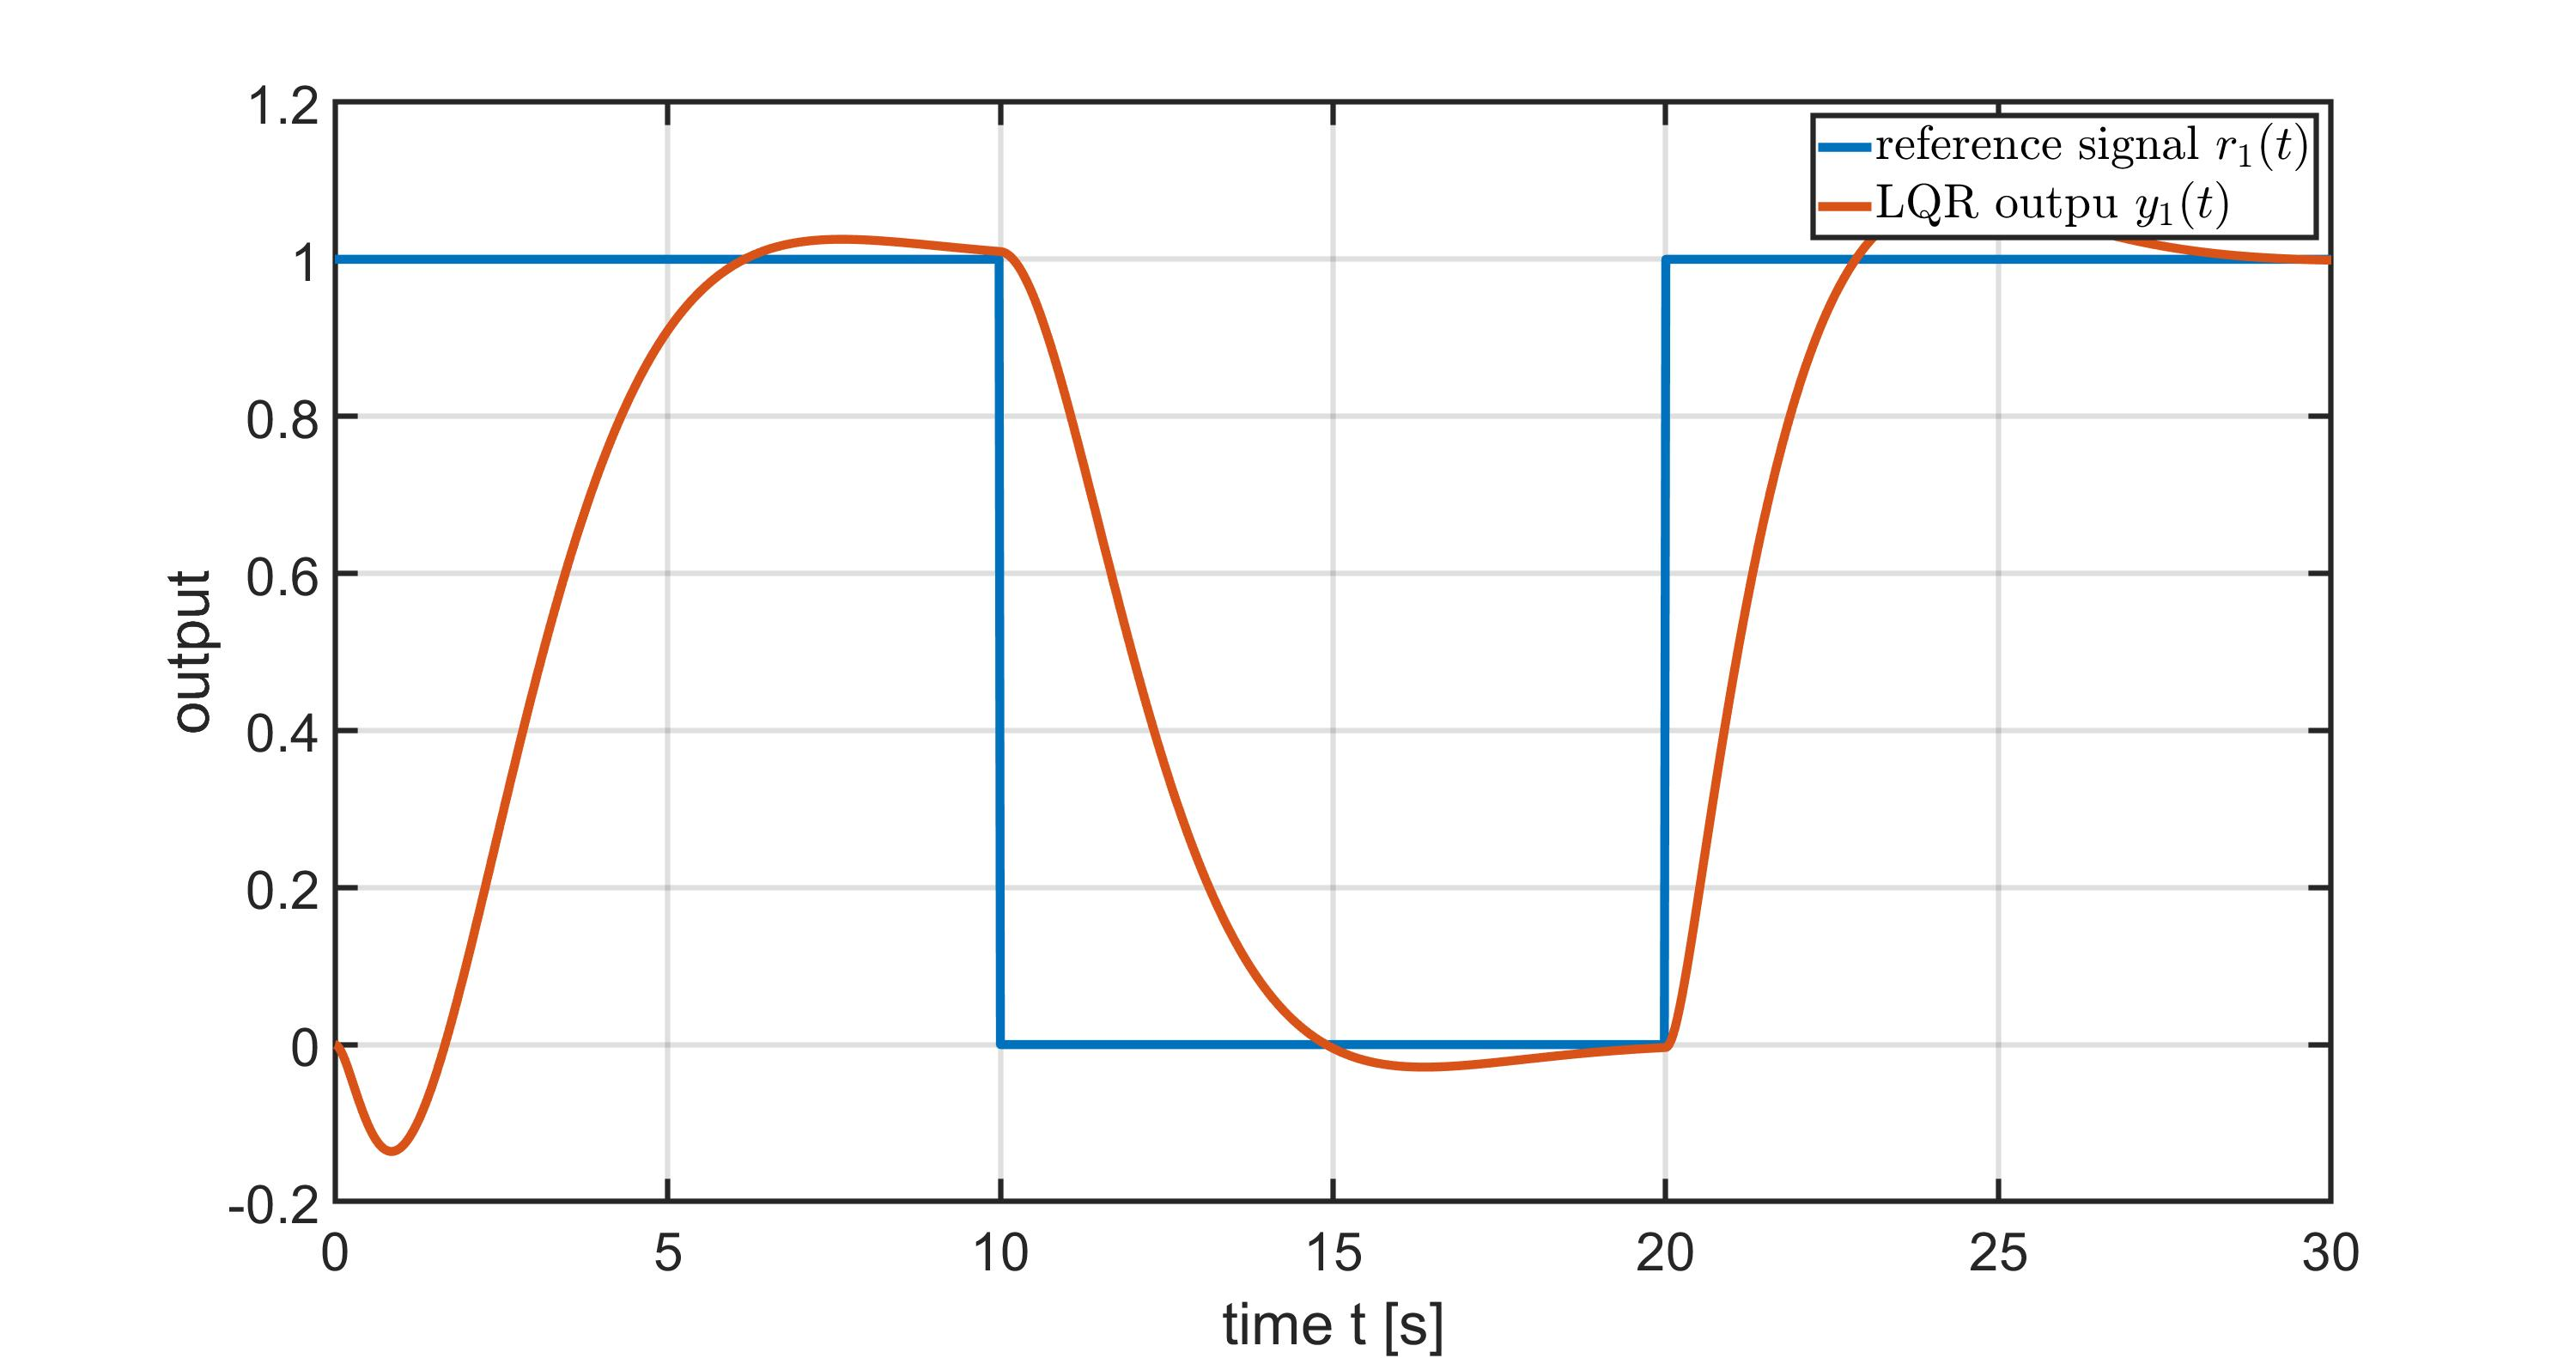
\includegraphics[width=\textwidth]{fig/AC1_LQR_1.jpg}
		\caption{First signal}
	\end{subfigure}
	\hfill
	\begin{subfigure}[b]{0.3\textwidth}
		\centering
		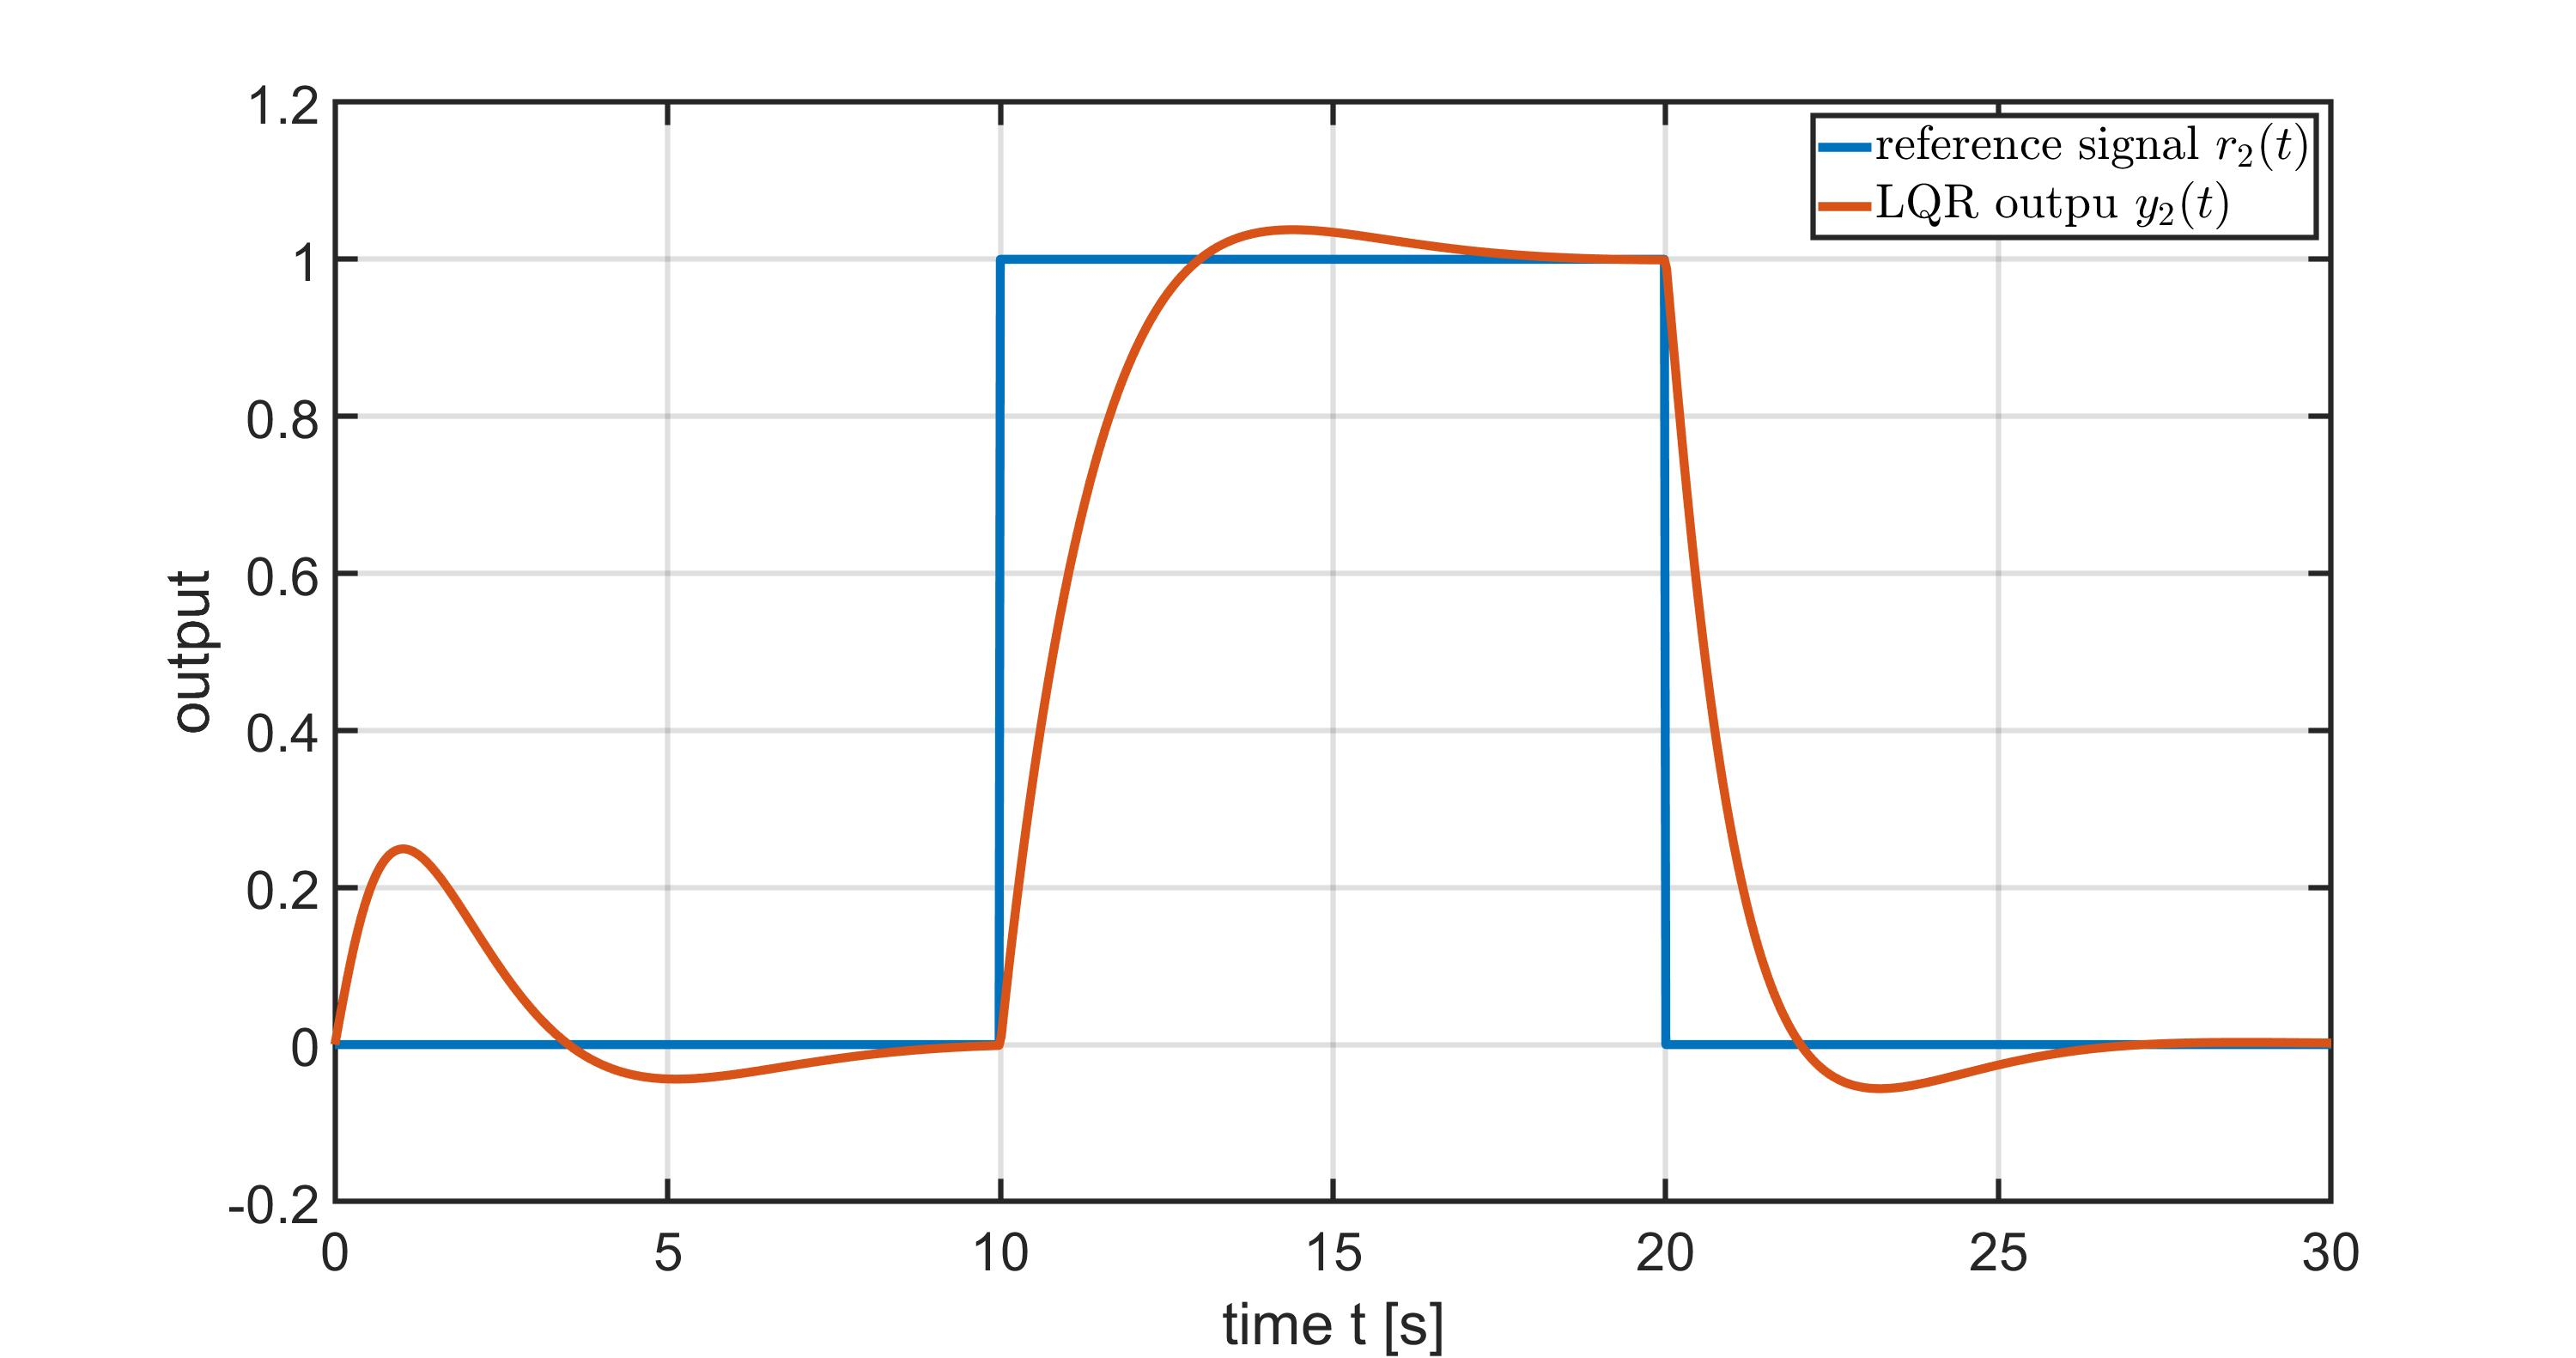
\includegraphics[width=\textwidth]{fig/AC1_LQR_2.jpg}
		\caption{Second signal}
	\end{subfigure}
	\hfill
	\begin{subfigure}[b]{0.3\textwidth}
		\centering
		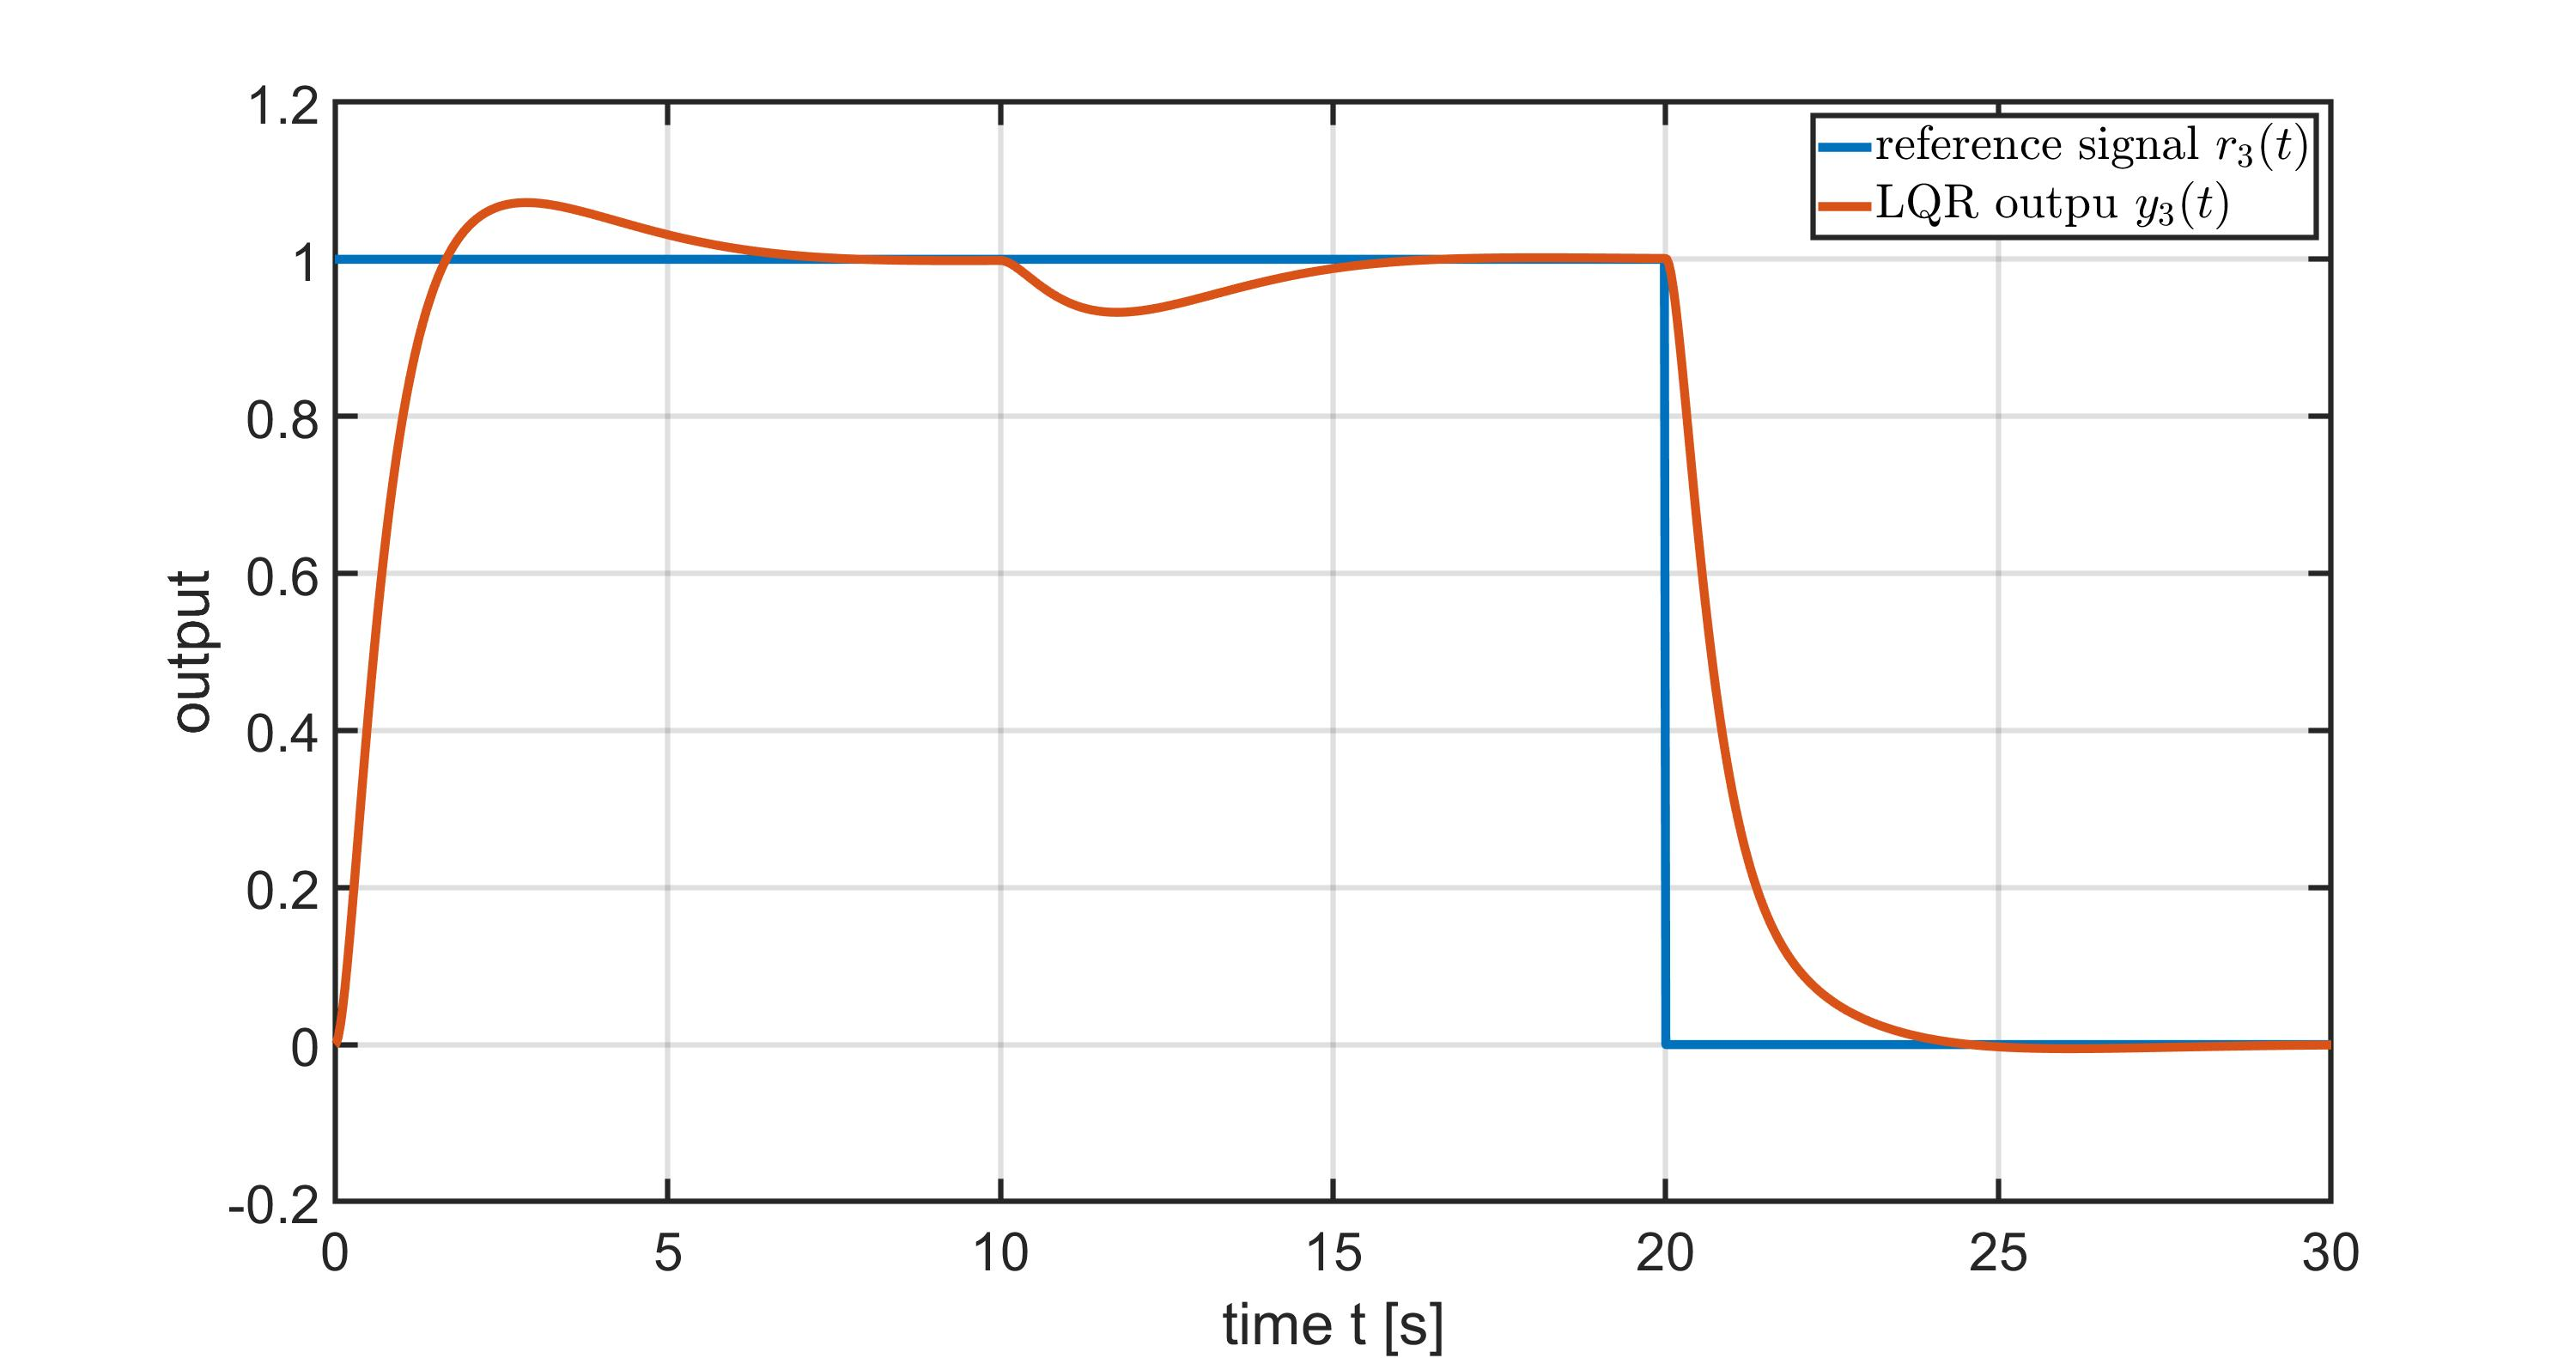
\includegraphics[width=\textwidth]{fig/AC1_LQR_3.jpg}
		\caption{Third signal}
	\end{subfigure}
	\caption{LQR tracking for the system \eqref{eq:Appl:discr_sys}}
	\label{img:Appl:AC1_LQR}
\end{figure}

It looks like something we can improve. However, for $Ts = 10^{-3}$s we get $N = 10^3$ time steps even for one simulation second. The resulting matrix $G$ can not easily be handled and needs vast masses of computer memory. 
\end{exam}

\section{Long time horizon}

	While in originally discrete systems the number of time steps can be not large (as each time step represents one iteration, which does not necessarily depends upon time), the discretezized continuous systems mostly have a large time horizon. 
	
	In Example \ref{ex:ILC:badIA} the Inverse Model Algorithm is not applicable even for $N = 50$. 
	It means, we need a trade off between the time horizon and robustness.
	Already for SISO system the matrix $G$ will have $(N + 1)^2$ elements. 
	
	The more obvious way to reduce the wasted memory is to use the sparse matrices. The matrix $G$ has a lower diagonal structure, what invites to save only the non-zero elements. Even a more space saving method is to save only the last ''line'' of the block matrices 
	\begin{align}
	G_{\rm{line}} = \begin{pmatrix}
	C A^{N-1} B & C A^{N-2} B & \dots & CB D
	\end{pmatrix}.
	\end{align}
	For SDA the matrix $G^\star$ can be perfectly calculated from this simplified form. However, the eigenvalues of the matrix $H$ can not as easily be calculated. However, we can estimate the norm of the matrix $G G^\star$, and choose $\beta$ from a possibly smaller region. 
	
	The solution for PIA  is a bit more complicated. 
	
	
	
	
	
	
	One possibility to reduce the wasted memory is to split our system in the smaller ones. Let us denote the time horizon length with $N_{\max}$, and choose an $N$ with $1<N\leq N_{\max}$
	We can apply our algorithms on the systems with the same state space description, but different initial values. For simplicity, let us assume, that we can divide our time horizon $0,1,2,\dots, N_{\max}$ in $p$ equal parts with time horizon of length $N$\footnote{In a more general case, where $N_{\max}$ can not be devided by $p$ without reminder, We can apply the algorithm one more time on the rest elements, or add them to the last applying iteration of the algorithm.}.  
	
	Then after we  $N$ iterations, we get for the next $N$ iterations the initial condition
	\begin{align}
	x_{0_{\rm{1}}} = A^{N} x(0) + \sum_{\tau = 0}^N A^{\tau}B u(N - \tau). 
	\end{align}
	
	For the next pass we adjust the next initial value as 
	\begin{align}
	x_{0_{\rm{2}}} = A^{2N} x(0) + \sum_{\tau = 0}^{2N} A^{\tau}B u(t - \tau) = A^N x(N+1) + \sum_{\tau = 0}^N A^{\tau} B u(2N - \tau). 
	\end{align}
	
	Doing so fare $1 \leq p^* \leq p$ algorithm passes, we get 
	\begin{align}
	\label{eq:Appl:new_x0}
	\begin{split}
	x_{0_{p^*}} =& A^N x((N+1)(p^* - 1)) + \sum_{\tau = 0}^N A^{\tau}B u(p^*N - \tau) \\
	=&  A^N x_{0_{p^* - 1}} + \sum_{\tau = 0}^N A^{\tau}B u(p^*N - \tau).
	\end{split}	
	\end{align}
	
	That means, we have no need to calculate even more than $N$ powers of $A$. 
	
	However, if the matrix is asymptotically stable, it might have an advantage to neglect some terms $C A^p B$ for $1<p<N$ large enough. 
	It allows us to skip the little elements of the matrix $G$, which might lead to bad condition number. 

	Another benefit of small terms neglecting is the use of sparse matrices. 	
	Our matrix $G$ has a lower triangular structure, and even without any neglecting we can decrease the memory usage by saving only the elements of $G$, which are not zero. With ''reduced'' matrix $G$ we can maintain more space and hence choose a larger $N$ to divide our system in.
	
	The following theorem illustrates it and supposes a method for choosing of this $p^*$. 
	
	\begin{theo}
		\label{thm:Appl:redSys}
	We consider the ''reduced'' lifted system 
	\begin{align}
	\t y = \t G u + d, 
	\end{align}
	\begin{align}
	\t G = \begin{pmatrix}
	D  \\
	CB & D \\
	C A B & CB & D\\
	\vdots & \vdots & \vdots & \ddots \\
	C A^{p^\star-1} B & C A^{p^\star-2}B & C A^{p^\star-3}B &\dots& D \\
	0           & C A^{p^\star-1} B & C A^{p^\star-2} B & \dots & CB & D\\
	0 & 0 & C A^{p^\star-1} B & \dots & CAB & CB & D \\
	\vdots & \vdots & \vdots & \ddots & \vdots & \vdots & \vdots & \ddots \\
	0 & 0 & 0 & \dots & C A^{p^\star-1}& C A^{p^\star-2}B& CA^{p^\star-3}B &\dots & D
	\end{pmatrix}.
	\end{align}
	If $||A||<1$, the error $||y(t) - \t y(t)||$, $p^* < t$, can be estimated undepended on $t$ as 
	\begin{align}
	||y(t) - \t y(t)|| < 2 ||C|| \, ||B|| \,  ||A||^{p^*}\, ||(I - A)^{-1}||\,||u_{\max}||, 
	\end{align}
	with 
	\begin{align}
	||u_{\max}|| = \max_{\tau = 0}^{t - p^*} ||u(\tau)||. 
	\end{align}
	
	$||\cdot||$ denotes here any vector norm and the corresponding induced matrix norm. 

	\end{theo}	
	\begin{proof}
	As $||A||<1$, all the eigenvalues of $A$ are less than 1 in its absolute value and hence the inverse of $(I - A)$ exists. Simple calculation provides 
		\begin{align}
	\begin{split}
			||y(t) - \t y(t)|| &= ||C \sum_{\tau = p^*}^t A^\tau B u(\tau)|| \leq ||C|| \, ||\sum_{\tau = p^*}^t A^\tau || \,||B|| \, ||u_{\max}|| \\
			& = ||C|| \, ||B|| \, ||(A^{p^*} - A^{t + 1})(I - A)^{-1}|| \, ||u_{\max}|| \\
			&  \leq 2 ||C|| \, ||B|| \, ||A||^{p^*} \, ||(I - A)^{-1}|| \, ||u_{\max}||. 
	\end{split}
		\end{align}
	\end{proof}


	This theorem says, that it does not matter how large is our $N$: we still can estimate our output with the same $p^*$. 
	Thou this estimation requires the systems to be asymptotically stable and the norm of the matrix $A$ should be less than one. In addition, this estimation is not very precise, and hence we can not apply this theorem to any system. 
	
	\begin{exam}
		Four our system \eqref{eq:ILC:Sys_ex1} we have for $||u_{\max}||\leq 1.5$ 
		$||y(t) - \t y(t)|| < 3.4033\, 10^{-11}$ for $N = 40$. Hence, we can apply the algorithms for very long time horizon without getting a large error. 
		
		TODO: Beispiel 
		
	\end{exam}

\begin{exam}
	\label{ex:Appl:redN}
	For example \eqref{eq:Appl:satellite_sys} we can not easily apply Theorem \ref{thm:Appl:redSys}: for $p^* = 10 \, 000 $ the estimation refers 
	\begin{align}
	||y(t) - \t y(t)|| \leq 0.8879 \text{ for } p^* < t < N,
	\end{align}
	if $||u_{\max}|| \leq 1$.
	
	One can also try to adapt the controller, such that the closed loop matrix $A$ has the eigenvalues of smaller absolute value. However, in our case it does not seem to be a better solution: $H_\infty$ design does not provide a better applicable solution, and pole placement yields the matrix $F$ with very large values. 
	
	But we still can divide our system in the smaller parts and apply the formula \eqref{eq:Appl:new_x0}. 
	
	Choose $N = 100$, and simulate the system dynamics for 30 seconds with time step of $10^{-3}$. 

But before we illustrate the result, let us consider one more issue. 
	
	
\end{exam}

\section{Online and Offline learning}

In the real problems we often can not have all the information immediately. If we apply the input sequences on the real system, we might have only the results at current time step and the previous ones. 

This is the difference between online and offline learning. In online mode we only have the information from previous iterations. We can not see in the feature and know what results we will get. In opposite, with offline learning we first calculate the new input sequence with an algorithm, and after that send the calculated result into the system and obtain the output. 

In the case of offline learning no more modification are required. We can discretize the system if it is required, split it in the smaller intervals and apply the algorithms. Especially for simulation this might be a good solution, as we can improve the whole sequence at once. 

The online learning requires a bit more effort. Here we apply a chosen ILC algorithm at each time step. This might need more iterations as offline learning, but still the number might rise not too large: since w already applied the algorithm on te previous steps, the new approach should probably need less trials. 

For online learning, the following pseudo code can be used: 
\begin{lstlisting}
x0new = x0
for i = 1 to N 
	x0new = A x0new + B u(i)
	unew = ILC(S, x0, i)
	u(1:i) = unew
end for

for i = N+1 to Nmax
	x0 := A x0new + B u(i) 
	unew = ILC(S, x0, N)
	u(i-N:i) = unew
end for
\end{lstlisting}	

$ILC(S, x0, k)$
 represents here an ILC algorithm over a system $S$, with initial condition $x_0$ and with $k$ -- given time horizon. 


\begin{exam}
	We continue Example \ref{ex:Appl:redN}, and apply the online learning on it. 
	The result for IA is illustrrated in the figure TODO. 
\end{exam}
	
	
	
	
%\chapter{Examples}
Ein paar Beispiele, die ich spaeter in die Kapitel reinstelle. 

\begin{exam}
	\label{Ex:ex2}
	\begin{align}
	A = \begin{pmatrix}
	-.5 & 0 \\ 0 & -.3
	\end{pmatrix},
	\begin{pmatrix}   
	0 \\ 0
	\end{pmatrix}, N = 200. 
	\end{align}
	\begin{figure}[ht]
		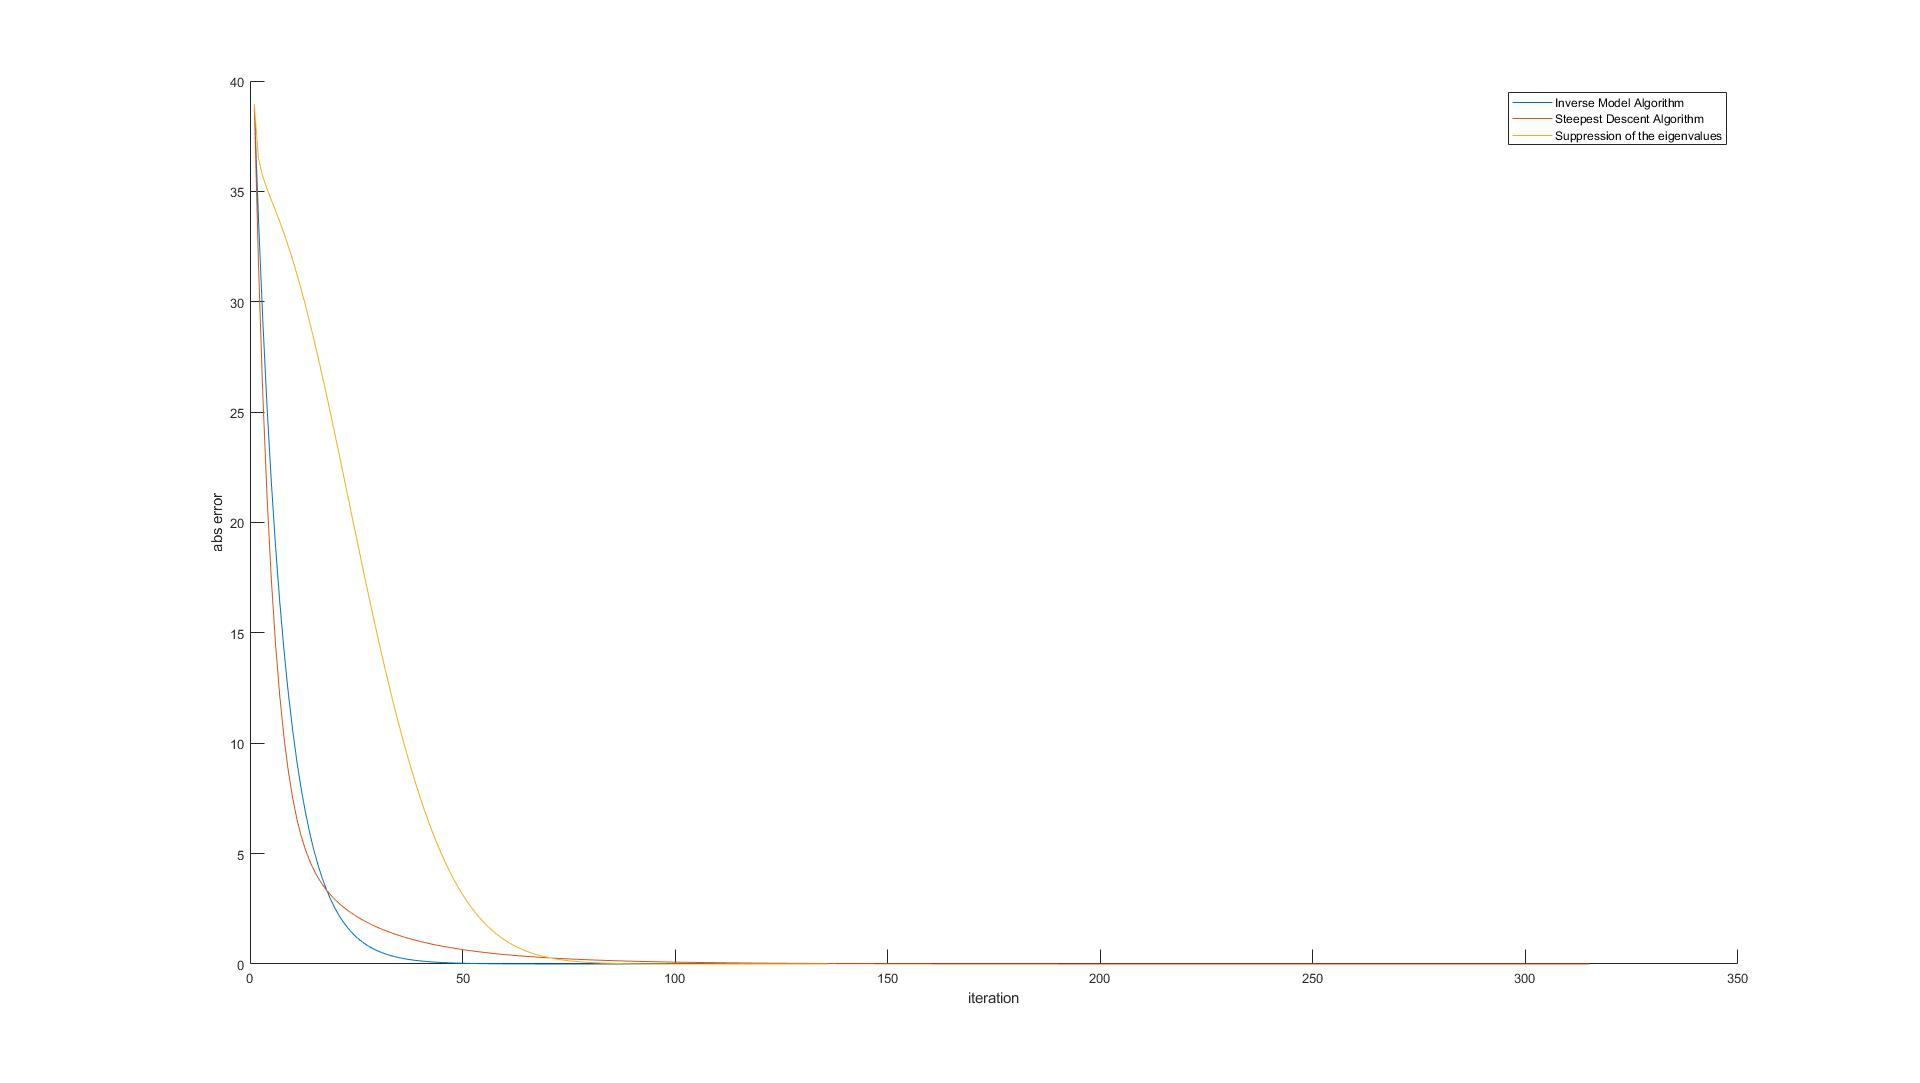
\includegraphics[width=\textwidth]{fig/Ex2.jpg}
		\caption{Example \ref{Ex:ex2}. $u_0 = .1$, $r(t)$ is random for $t = 0, 1, 2, \dots, N$.}
	\end{figure}	
\end{exam}

\begin{exam}
	Satellite Example
	\begin{figure}[ht]
		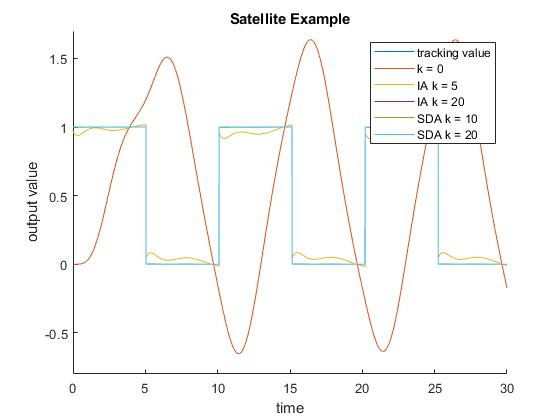
\includegraphics[width=\textwidth]{fig/SatelliteEx.jpg}
		\caption{}
	\end{figure}	
\end{exam}

\begin{exam}
	\label{ex:Unc}
	Uncertain Example
	\begin{align}
	A = \begin{pmatrix}
	-.5 + a & 0 \\ 0 & -.4-a
	\end{pmatrix}, 
	B = \begin{pmatrix}
	1 \\ 1
	\end{pmatrix}, 
	C = \begin{pmatrix}
	.1 & .2
	\end{pmatrix},
	D = 1. x_0 = \begin{pmatrix}
	0 \\ 0
	\end{pmatrix}, N = 200. 
	\end{align}
	$a$ is an uncertain parameter with nominal value $\hat{a} = 1.5$ and variability $a \in [1.3, \; 1.8]$.
	\begin{figure}[ht]
		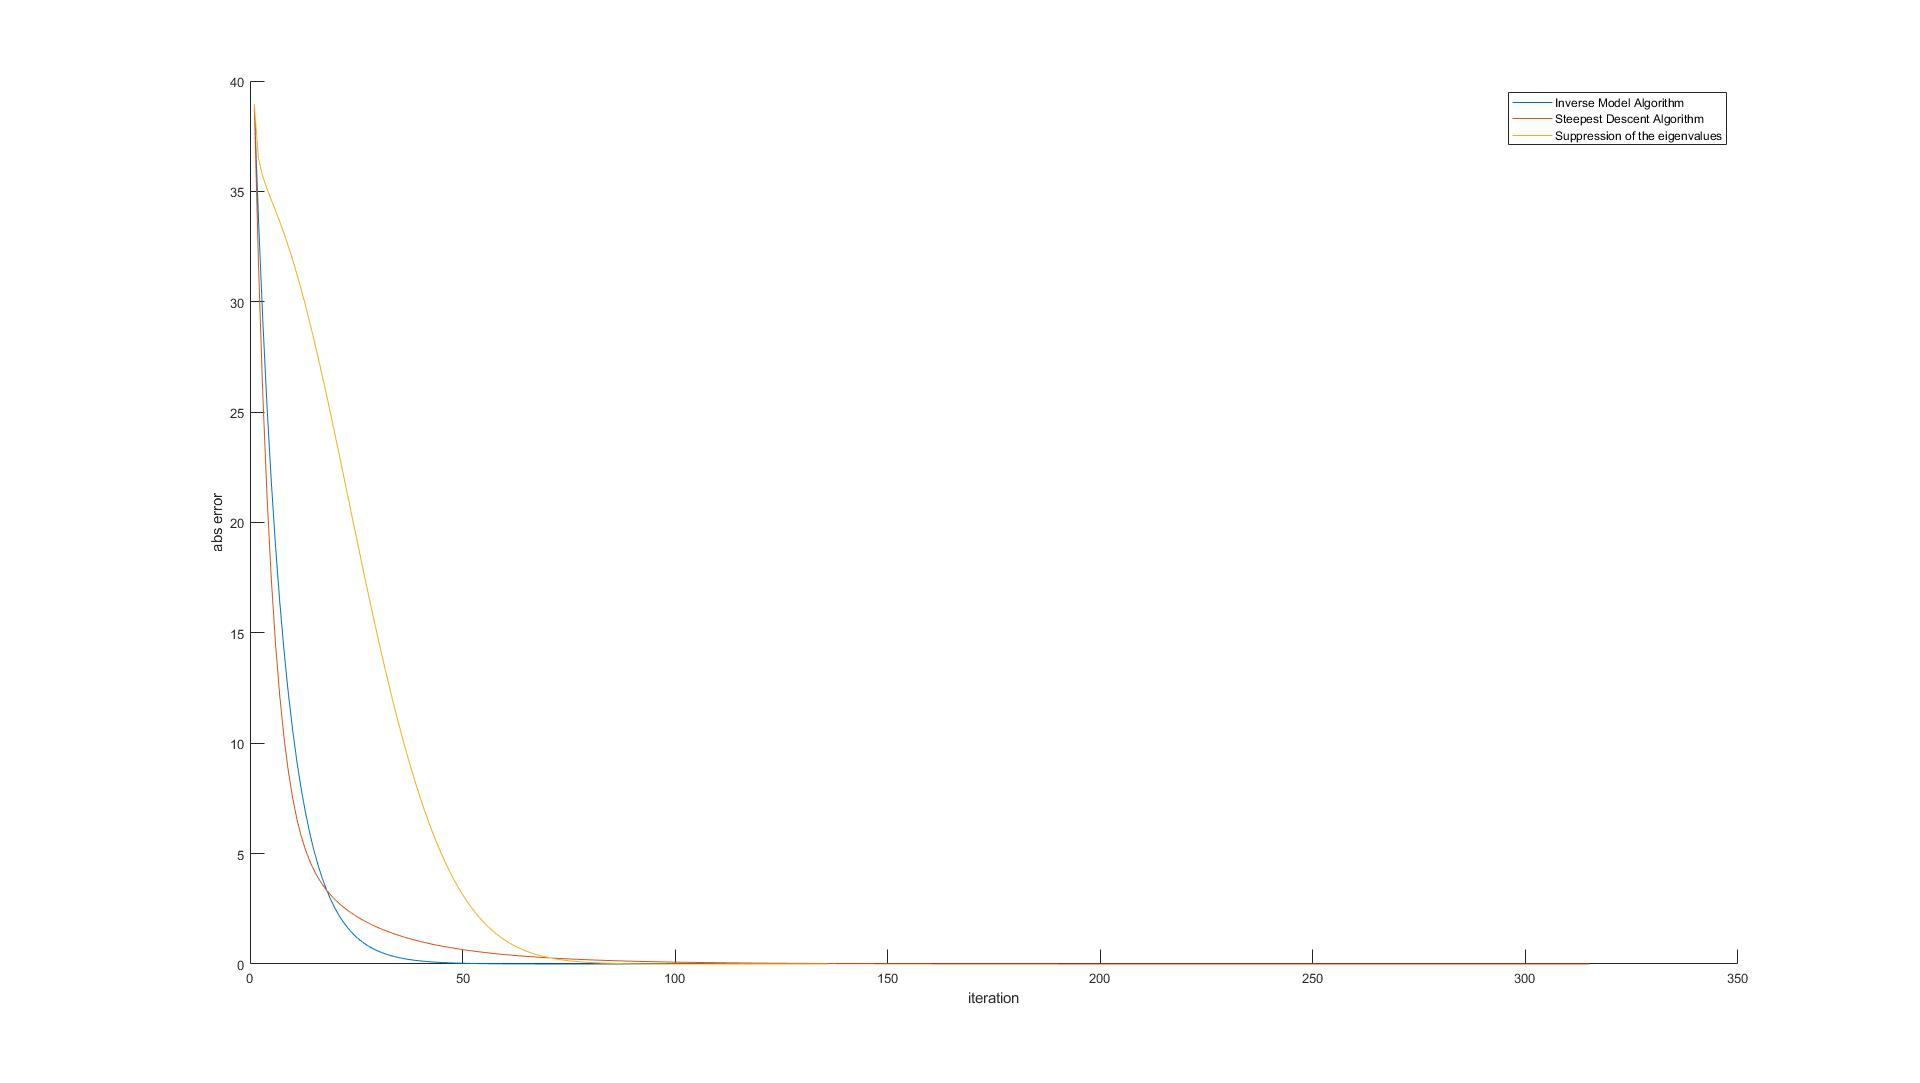
\includegraphics[width=\textwidth]{fig/Ex2.jpg}
		\caption{Example \ref{ex:Unc}. $u(0) = .1$, $r(t)$ is random for $t = 0, 1, 2, \dots, N$.}
	\end{figure}	
\end{exam}
%\begin{figure}
	\begin{center}
		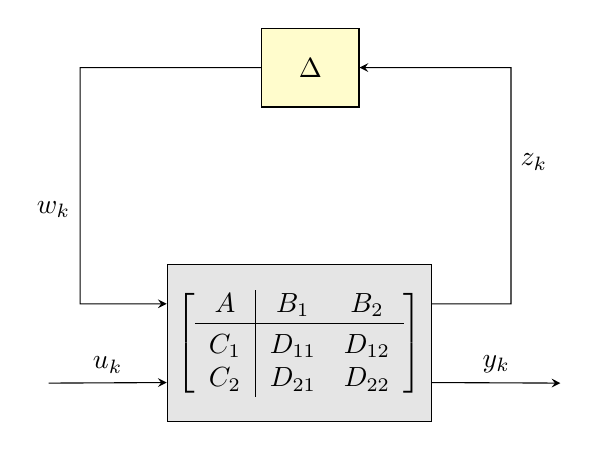
\begin{tikzpicture}[>=stealth]
		%coordinates
		\coordinate (orig)   at (0,0);

		\coordinate (AroneA) at (-3,1.5);
		\coordinate (ArtwoA) at (5,.5);
		\coordinate (ArthrA) at (-1.5,.5);
		\coordinate (LLA)    at (0,0);
		\coordinate (LLD)    at (1.2,4);
	
		%nodes
		\node[draw, minimum width=2cm, minimum height=2cm, anchor=south west, align=center, fill = gray!20] (A) at (LLA) {$\left[\begin{array}{c|c c}
			A & B_1 & B_2 \\\hline C_1 & D_{11} & D_{12} \\ C_2 & D_{21} & D_{22}
			\end{array}\right]$};
		\node[draw, minimum width=1.2cm, minimum height=1cm, anchor=south west, text width=1cm, align=center ,fill = yellow!20] (D) at (LLD) {$\Delta$};

		\draw[->] (ArthrA) -- node[above]{$u_k$} ($(A.180) + (0,-1/2)$);
		\draw[->]  ($(A.east) - (0,.5)$) -- node[above]{$y_{k}$}(ArtwoA);
		
		\draw[->] ($(A.0) + (0,1/2)$) -| ++ (1,1.5) -- node[right, pos=0.2]{$z_k$}++ (0,1.5) -- ($(D.east)$);		
		\draw[->] ($(D.west)$) -| ++ (-2.3,-1.5) -- node[left, pos=0.2]{$w_k$} ++ (0,-1.5) -- ($(A.180) + (0,1/2)$);
		\end{tikzpicture}
		
	\end{center}
	
\end{figure}



\begin{figure}
	\begin{center}
		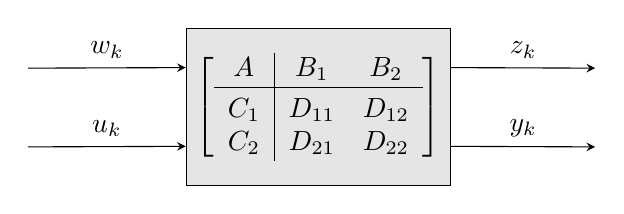
\begin{tikzpicture}[>=stealth]
		%coordinates
		\coordinate (orig)   at (0,0);
		
		\coordinate (AroneA) at (-3,1.5);
		\coordinate (ArtwoA) at (5.2,.5);
		\coordinate (ArthrA) at (-2,.5);
		\coordinate (ArfA) at (-2,1.5);
		\coordinate (ArfiveA) at (5.2,1.5);		
		\coordinate (LLA)    at (0,0);
		\coordinate (LLD)    at (.51,4);
		
		%nodes
		\node[draw, minimum width=2cm, minimum height=2cm, anchor=south west,  align=center, fill = gray!20] (A) at (LLA) {$\left[\begin{array}{c|c c}
			A & B_1 & B_2 \\\hline C_1 & D_{11} & D_{12} \\ C_2 & D_{21} & D_{22}
			\end{array}\right]$};
%		\node[draw, minimum width=1.2cm, minimum height=1cm, anchor=south west, text width=1cm, align=center ,fill = yellow!20] (D) at (LLD) {$\Delta$};
		
		\draw[->] (ArthrA) -- node[above]{$u_k$} ($(A.180) + (0,-1/2)$);
		\draw[->]  ($(A.east) - (0,.5)$) -- node[above]{$y_k$}(ArtwoA);
		
		\draw[->] (ArfA) -- node[above]{$w_k$} ($(A.180) - (0,-1/2)$);
		\draw[->]  ($(A.east) + (0,.5)$) -- node[above]{$z_k$}(ArfiveA);
		
%		\draw[->] ($(A.0) + (0,1/2)$) -| ++ (1,1.5) -- node[right, pos=0.2]{$z_k$}++ (0,1.5) -- ($(D.east)$);		
%		\draw[->] ($(D.west)$) -| ++ (-1.5,-1.5) -- node[left, pos=0.2]{$w_k$} ++ (0,-1.5) -- ($(A.180) + (0,1/2)$);
		\end{tikzpicture}
	\end{center}
	\caption{Linear Fractional Representation: open loop}
\end{figure}



\begin{figure}
	\begin{center}
		\begin{subfigure}{.5\textwidth}
			\centering 			
			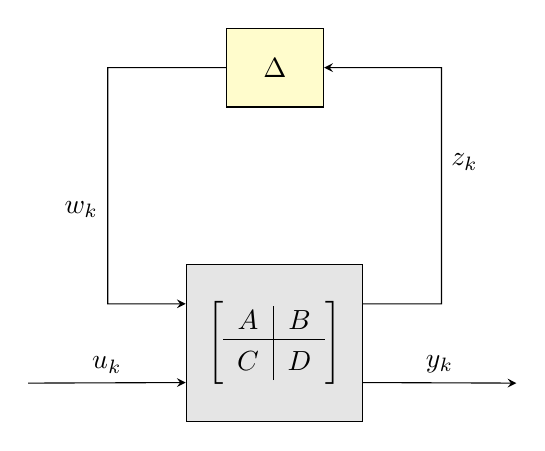
\begin{tikzpicture}[>=stealth]
			%coordinates
			\coordinate (orig)   at (0,0);
			
			\coordinate (AroneA) at (-3,1.5);
			\coordinate (ArtwoA) at (4.2,.5);
			\coordinate (ArthrA) at (-2,.5);
			\coordinate (LLA)    at (0,0);
			\coordinate (LLD)    at (.51,4);
			
			%nodes
			\node[draw, minimum width=2cm, minimum height=2cm, anchor=south west, text width=2cm, align=center, fill = gray!20] (A) at (LLA) {$\left[\begin{array}{c|c}
				A & B \\\hline C & D
				\end{array}\right]$};
			\node[draw, minimum width=1.2cm, minimum height=1cm, anchor=south west, text width=1cm, align=center ,fill = yellow!20] (D) at (LLD) {$\Delta$};
			
			\draw[->] (ArthrA) -- node[above]{$u_k$} ($(A.180) + (0,-1/2)$);
			\draw[->]  ($(A.east) - (0,.5)$) -- node[above]{$y_k$}(ArtwoA);
			
			\draw[->] ($(A.0) + (0,1/2)$) -| ++ (1,1.5) -- node[right, pos=0.2]{$z_k$}++ (0,1.5) -- ($(D.east)$);		
			\draw[->] ($(D.west)$) -| ++ (-1.5,-1.5) -- node[left, pos=0.2]{$w_k$} ++ (0,-1.5) -- ($(A.180) + (0,1/2)$);
			\end{tikzpicture} \caption{Closed loop}
		\end{subfigure}
		\vspace{1cm}
		
		\begin{subfigure}{.5\textwidth}
			\centering
			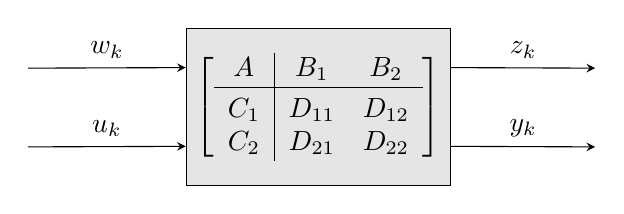
\begin{tikzpicture}[>=stealth]
			%coordinates
			\coordinate (orig)   at (0,0);
			
			\coordinate (AroneA) at (-3,1.5);
			\coordinate (ArtwoA) at (5.2,.5);
			\coordinate (ArthrA) at (-2,.5);
			\coordinate (ArfA) at (-2,1.5);
			\coordinate (ArfiveA) at (5.2,1.5);		
			\coordinate (LLA)    at (0,0);
			\coordinate (LLD)    at (.51,4);
			
			%nodes
			\node[draw, minimum width=2cm, minimum height=2cm, anchor=south west,  align=center, fill = gray!20] (A) at (LLA) {$\left[\begin{array}{c|c c}
				A & B_1 & B_2 \\\hline C_1 & D_{11} & D_{12} \\ C_2 & D_{21} & D_{22}
				\end{array}\right]$};
			%		\node[draw, minimum width=1.2cm, minimum height=1cm, anchor=south west, text width=1cm, align=center ,fill = yellow!20] (D) at (LLD) {$\Delta$};
			
			\draw[->] (ArthrA) -- node[above]{$u_k$} ($(A.180) + (0,-1/2)$);
			\draw[->]  ($(A.east) - (0,.5)$) -- node[above]{$y_k$}(ArtwoA);
			
			\draw[->] (ArfA) -- node[above]{$w_k$} ($(A.180) - (0,-1/2)$);
			\draw[->]  ($(A.east) + (0,.5)$) -- node[above]{$z_k$}(ArfiveA);
			
			%		\draw[->] ($(A.0) + (0,1/2)$) -| ++ (1,1.5) -- node[right, pos=0.2]{$z_k$}++ (0,1.5) -- ($(D.east)$);		
			%		\draw[->] ($(D.west)$) -| ++ (-1.5,-1.5) -- node[left, pos=0.2]{$w_k$} ++ (0,-1.5) -- ($(A.180) + (0,1/2)$);
			\end{tikzpicture}
			\caption{Open loop}
		\end{subfigure}
		
	\end{center}
	\caption{Linear Fractional Representation}
\end{figure}
\chapter{Questions} 



%\begin{figure}
%	\begin{center}
%		\begin{tikzpicture}[>=stealth]
%		%coordinates
%
%		%nodes
%		\node[draw, minimum width=2cm, minimum height=2cm, anchor=south west, align=center, fill = gray!20](G){$G$};
%		\node[draw, below = of G,minimum width=1cm, minimum height=1cm](K){$K$};
%		
%		\node[draw, fit = (G)(K)](Gt){}; 		
%		
%		\node[draw, below = of Gt,minimum width=1cm, minimum height=1cm](tK){$\t K$};
%		
%		\draw[->](G.170)--($(G.170) + (-1,0)$)node[left]{$-e$};
%		\draw[->](G.190)--($(G.190) + (-1,0)$)node[left]{$e$} |-(K.180);
%		\draw[->](G.190)--($(G.190) + (-1,0)$)node[left]{} |-(tK.180);
%		
%		\draw[->](K.180)--($(G.190) + (-1,0)$)node[left]{} |-(tK.180);
%		
%		
%		
%		
%
%		\end{tikzpicture}
%		
%	\end{center}
%	\caption{} 
%\end{figure}



%
%
%For SDA: 
%
%\begin{align}
%\begin{pmatrix}
%y_1 \\ y_2
%\end{pmatrix} = \begin{pmatrix}
%G_1 & 0 \\ G_3 & G_1
%\end{pmatrix}\begin{pmatrix}
%u_1 \\ u_2 
%\end{pmatrix} + \begin{pmatrix}
%d_1\\d_2
%\end{pmatrix}.
%\end{align}
%
%\begin{align}
%\begin{pmatrix}
%u_1 \\ u_2
%\end{pmatrix}_{k+1} =
%\begin{pmatrix}
%u_1 \\ u_2
%\end{pmatrix}_k + 
%\begin{pmatrix}
%G_1^* & G_3^* \\0 & G_1^*
%\end{pmatrix}\begin{pmatrix}
%e_1 \\ e_2
%\end{pmatrix}_k.
%\end{align}
%
%\begin{align*}
%\begin{split}
%G &= G(A,B,C,D) = \\
%&=  \begin{pmatrix}
%D & 0 & \cdots & 0 & 0 & 0 \\
%CB & D & \cdots & 0 & 0 & 0\\
%CAB & CB & \cdots & 0 & 0 & 0\\
%\vdots & \vdots & \ddots & \vdots  & \vdots & \vdots \\
%CA^{N-2} B & CA^{N-3} B &\dots &CB & D& 0\\
%CA^{N-1} B & CA^{N-2} B &\dots &CAB & CB& D\\
%\end{pmatrix} \in \R^{m(N+1)\times l(N+1)}.
%\end{split}
%\end{align*}
%
%\begin{align}
%\begin{pmatrix}
%\dot x \\\dot x_K\\
%z \\
%y_K\\
%y
%\end{pmatrix}
%= 
%\begin{pmatrix}
%A x + B_1 w + B_2 u + B_2 v\\
%... \\...\\...\\...
%\end{pmatrix}
%\end{align}
%
%
%
%
%


Hier k�nnen auch Schlu�folgerungen pr�sentiert und ein Ausblick gegeben werden.

%%%%%%%%%%%%%%%%%%%%%%%%%%%%%
% Literaturverzeichnis
%%%%%%%%%%%%%%%%%%%%%%%%%%%%%
%\newpage
%\newpage\pagenumbering{Roman}
%\setcounter{page}{5}

%\bibliography{ProjectILC}
\printbibliography



%%%%%%%%%%%%%%%%%%%%%%%%%%%%%
% APPENDIX 
%%%%%%%%%%%%%%%%%%%%%%%%%%%%%
\newpage\clearpage
\addcontentsline{toc}{section}{Anhang}
\begin{appendix}

%-------------------------------------------------------------------------------
\section{Beweise}\sectionmark{Beweise}
%-------------------------------------------------------------------------------

%-------------------------------------------------------------------------------
\subsection{Beweis 1}
%-------------------------------------------------------------------------------

\begin{eqnarray}
1+1 = 2
\end{eqnarray}

\end{appendix}



%%%%%%%%%%%%%%%%%%%%%%%%%%%%%
%  Eidesstattliche Erkl�rung
%%%%%%%%%%%%%%%%%%%%%%%%%%%%%
\newpage
\section*{Eidesstattliche Erkl�rung}\sectionmark{Eidesstattliche Erkl�rung}
\addcontentsline{toc}{section}{Eidesstattliche Erkl�rung}%\addtocontents{toc}{\vfill}
Ich erkl�re, dass ich meine Bachelor-Arbeit [\emph{Titel der Arbeit}] selbstst�ndig und ohne Benutzung anderer als der angegebenen Hilfsmittel angefertigt habe und dass ich alle Stellen, die ich w�rtlich oder sinngem�� aus Ver�ffentlichungen entnommen habe, als solche kenntlich gemacht habe. Die Arbeit hat bisher in gleicher oder �hnlicher Form oder auszugsweise noch keiner Pr�fungsbeh�rde vorgelegen. \\
%\\
%Ich versichere, dass die eingereichte schriftliche Fassung der auf dem beigef�gten Medium gespeicherten Fassung entspricht.[\emph{Dieser Zusatz ist nur erforderlich, wenn die Abschlussarbeit auch als Datei abgegeben worden ist.}]\\\\\\
\noindent Stuttgart, den XX.XX.2013
\begin{flushright}
$\overline{~~~~~~~~~\mbox{(Name des Kandidaten)}~~~~~~~~~}$
\end{flushright}

%-------------------------------------------------------------------
\chapter{Zusammenfassung und Ausblick}
%-------------------------------------------------------------------------------



\end{document} 